\documentclass[12pt,a4paper,oneside]{report}
\setlength{\parindent}{0pt}  % tắt indent mặc định
\setlength{\parskip}{0pt}    % khoảng cách giữa các đoạn
%================= MÃ HÓA - NGÔN NGỮ =================
\usepackage[utf8]{inputenc}
\usepackage[T5]{fontenc}
\usepackage[vietnamese]{babel}
\usepackage{amsmath}
\usepackage{amssymb}
\usepackage{bm}
\usepackage{bbm}
\usepackage{dsfont}
\usepackage{multirow}
\usepackage{makecell}
\usepackage{float} 
\usepackage[unicode]{hyperref}
\usepackage{tikz}
\usetikzlibrary{shapes.geometric, arrows, positioning}
\usepackage{caption}
\usepackage{float}
\usepackage{titlesec}
\usetikzlibrary{calc, positioning, arrows.meta, backgrounds, angles, quotes, decorations.pathreplacing}

\titleformat{\subsubsection}[block]
  {\fontsize{13}{15}\selectfont\bfseries}
  {\thesubsubsection}{1em}{}
%================= FONT - TOÁN =================
% \usepackage{eulervm}
\usepackage{lmodern}


%================= HÌNH ẢNH - MÀU - KHUNG =================
\usepackage{graphicx}
\usepackage{xcolor}
\usepackage{tikz}
\usepackage{enumitem}
\usepackage{longtable}
%================= CĂN LỀ - GIÃN DÒNG =================
\usepackage{geometry}
\usepackage{setspace}
\usepackage{ragged2e}
\geometry{
    a4paper,
    top=2.5cm,
    bottom=2.5cm,
    left=3.5cm,
    right=2.0cm
}

\setstretch{1.3}
\setlength{\parindent}{0pt}  % tắt thụt đầu dòng mặc định
\setlength{\parskip}{0pt}    % khoảng cách giữa các đoạn
%\setlist[itemize]{leftmargin=2em,labelsep=0.5em}
%\setlist[enumerate]{leftmargin=2em,labelsep=0.5em}

%================= MỤC LỤC =================
\usepackage{tocloft}
\usepackage{fancyhdr}
\pagestyle{fancy}
\fancyhf{}
\fancyfoot[C]{\thepage}
\renewcommand{\headrulewidth}{0pt}

\fancypagestyle{plain}{
    \fancyhf{}
    \fancyfoot[C]{\thepage}
    \renewcommand{\headrulewidth}{0pt}
}
\renewcommand{\contentsname}{MỤC LỤC}
\renewcommand{\listfigurename}{Danh sách hình ảnh và biểu đồ}
\renewcommand{\listtablename}{Danh sách bảng}
\setcounter{tocdepth}{3}
\setcounter{secnumdepth}{3}

\renewcommand{\cftchapfont}{\bfseries}
\renewcommand{\cftchappagefont}{\bfseries}
\setlength{\cftbeforechapskip}{6pt}
\setlength{\cftbeforesecskip}{2pt}


%================= THÔNG TIN TÀI LIỆU =================
\newcommand{\tentruong}{TRƯỜNG ĐẠI HỌC ĐÀ LẠT}
\newcommand{\tenkhoa}{KHOA TOÁN - TIN HỌC}
\newcommand{\tendoan}{ĐỒ ÁN CƠ SỞ}
\newcommand{\tendetai}{TIẾP CẬN PHƯƠNG PHÁP LDA CỦA R.A. FISHER\\TRONG PHÂN LOẠI MẪU THỐNG KÊ}
\newcommand{\gvhdmot}{Đặng Phước Huy}
\newcommand{\gvhdhai}{Huỳnh Bảo Tuyên}
\newcommand{\svth}{Phùng Ngọc Bảo}
\newcommand{\mssv}{2212318}
\newcommand{\lop}{KLK46}
\newcommand{\noilam}{Lâm Đồng}
\newcommand{\thoigian}{tháng 6 năm 2026}

\begin{document}

%====================================================
%                   TRANG BÌA
%====================================================

\begin{titlepage}
	\thispagestyle{empty}
	
	\begin{tikzpicture}[remember picture, overlay]
		\draw[line width=0.8pt]
		([xshift=3.5cm,yshift=-2.5cm]current page.north west)
		rectangle
		([xshift=-2.0cm,yshift=2.5cm]current page.south east);
	\end{tikzpicture}
	
	\begin{center}
		\vspace*{0.3cm}
		
		{\bfseries\fontsize{15}{18}\selectfont \tentruong \par}
		\vspace{0.15cm}
		{\bfseries\fontsize{15}{18}\selectfont \tenkhoa \par}
		
		\vspace{1.0cm}
		
		
\includegraphics[width=3.4cm]{image/logo.png}
		
		\vspace{1.1cm}
		
		{\bfseries\fontsize{14}{20}\selectfont \tendoan \par}
		
		\vspace{2.8cm}
		
		{\bfseries\fontsize{13}{20}\selectfont\color{red!75!black}
			\tendetai \par}
		
		\vspace{2.8cm}
		
		\begin{flushleft}
			\hspace{5.8cm}Giảng viên hướng dẫn: \textbf\gvhdmot\\[0.35cm]
			\hspace{5.8cm}\phantom{Giảng viên hướng dẫn:} \textbf\gvhdhai\\[0.35cm]
			\hspace{5.8cm}Sinh viên thực hiện: \textbf{\svth}\\[0.35cm]
			\hspace{5.8cm}Mã số sinh viên: \textbf{\mssv}\\[0.35cm]
			\hspace{5.8cm}Lớp: \textbf{\lop}
		\end{flushleft}
		
		\vfill
		
		{\fontsize{13}{15}\selectfont \noilam, \thoigian \par}
	\end{center}
\end{titlepage}

%====================================================
%                   TRANG BÌA LÓT
%====================================================

\clearpage
\thispagestyle{empty}

\begin{tikzpicture}[remember picture, overlay]
	% Khung ngoài
	\draw[line width=1.5pt]
	([xshift=3.5cm,yshift=-2.0cm]current page.north west)
	rectangle
	([xshift=-2.0cm,yshift=2.0cm]current page.south east);
	
	% Khung trong
	\draw[line width=0.5pt]
	([xshift=3.65cm,yshift=-2.15cm]current page.north west)
	rectangle
	([xshift=-2.15cm,yshift=2.15cm]current page.south east);
\end{tikzpicture}

\begin{center}
	\vspace*{0.0cm}
	
	{\bfseries\fontsize{13}{16}\selectfont TRƯỜNG ĐẠI HỌC ĐÀ LẠT\par}
	\vspace{0.15cm}
	{\bfseries\fontsize{13}{16}\selectfont KHOA TOÁN -- TIN HỌC\par}
	
	\vspace{2.0cm}
	
	{\bfseries\fontsize{12}{15}\selectfont PHÙNG NGỌC BẢO -- 2212318\par}
	
	\vspace{1.5cm}
	
	\vspace{2.5cm}
	
	{\bfseries\fontsize{13}{20}\selectfont
		TIẾP CẬN PHƯƠNG PHÁP LDA CỦA R.A. FISHER\\
		TRONG PHÂN LOẠI MẪU THỐNG KÊ
		\par}
	
	\vspace{2.2cm}
	
	{\bfseries\fontsize{13}{20}\selectfont ĐỒ ÁN CƠ SỞ\par}
	
	\vspace{2.6cm}
	
	{\bfseries\fontsize{12}{16}\selectfont
		GIẢNG VIÊN HƯỚNG DẪN\\
		ĐẶNG PHƯỚC HUY\\
		HUỲNH BẢO TUYÊN
		\par}
	
	\vfill
	
	{\fontsize{12}{16}\selectfont LÂM ĐỒNG, NĂM 2026\par}
	
	\vspace*{0.5cm}
\end{center}

\clearpage
%====================================================
%               PHẦN ĐẦU LUẬN VĂN
%====================================================
\clearpage
\pagenumbering{roman}
\setcounter{page}{1}
%====================================================
%               PHẦN NHẬN XÉT CỦA GIÁNG VIÊN
%====================================================

%\clearpage
%\thispagestyle{plain}
%
%\begin{center}
%    \textbf{\fontsize{16}{18}\selectfont NHẬN XÉT CỦA GIẢNG VIÊN HƯỚNG DẪN 1}
%\end{center}
%
%\vspace{0.5cm}
%
%\noindent Họ và tên sinh viên: \textbf{Phùng Ngọc Bảo}\\[0.3cm]
%\noindent Mã số sinh viên: \textbf{2212318}\\[0.3cm]
%\noindent Lớp: \textbf{KLK46}\\[0.4cm]
%
%\noindent Tên đề tài:\\
%\textit{Tiếp cận phương pháp LDA của R.A. Fisher trong phân loại mẫu thống kê}
%
%\vspace{0.5cm}
%
%\noindent \textbf{Nội dung nhận xét:}
%
%
%\vspace{0.4cm}
%
%\newcommand{\nhanxetline}{\noindent\makebox[\textwidth][l]{\rule{1\textwidth}{0.4pt}}\\[0.4cm]}
%
%\nhanxetline
%\nhanxetline
%\nhanxetline
%\nhanxetline
%\nhanxetline
%\nhanxetline
%
%\vspace{0.0cm}
%
%\noindent \textbf{Đánh giá:}
%
%\vspace{0.0cm}
%
%\nhanxetline
%\nhanxetline
%
%\vspace{0.0cm}
%
%\begin{flushright}
%\textnormal{Lâm Đồng, ngày \hspace{1cm} tháng \hspace{1cm} năm 2026}\\[0.8cm]
%\textbf{Giảng viên hướng dẫn}\\[2.6cm]
%\textbf{(Ký và ghi rõ họ tên)}
%\end{flushright}
%
%
%%====================================================
%%               PHẦN NHẬN XÉT CỦA GIÁNG VIÊN
%%====================================================
%
%\clearpage
%\thispagestyle{plain}
%
%\begin{center}
%    \textbf{\fontsize{16}{18}\selectfont NHẬN XÉT CỦA GIẢNG VIÊN HƯỚNG DẪN 2}
%\end{center}
%
%\vspace{0.5cm}
%
%\noindent Họ và tên sinh viên: \textbf{Phùng Ngọc Bảo}\\[0.3cm]
%\noindent Mã số sinh viên: \textbf{2212318}\\[0.3cm]
%\noindent Lớp: \textbf{KLK46}\\[0.4cm]
%
%\noindent Tên đề tài:\\
%\textit{Tiếp cận phương pháp LDA của R.A. Fisher trong phân loại mẫu thống kê}
%
%\vspace{0.5cm}
%
%\noindent \textbf{Nội dung nhận xét:}
%
%
%\vspace{0.4cm}
%
%\nhanxetline
%\nhanxetline
%\nhanxetline
%\nhanxetline
%\nhanxetline
%\nhanxetline
%
%\vspace{0.0cm}
%
%\noindent \textbf{Đánh giá:}
%
%\vspace{0.0cm}
%
%\nhanxetline
%\nhanxetline
%
%\vspace{0.0cm}
%
%\begin{flushright}
%\textnormal{Lâm Đồng, ngày \hspace{1cm} tháng \hspace{1cm} năm 2026}\\[0.8cm]
%\textbf{Giảng viên hướng dẫn}\\[2.6cm]
%\textbf{(Ký và ghi rõ họ tên)}
%\end{flushright}
%
%%====================================================
%%               LỜI CAM ĐOAN
%%====================================================
%\clearpage
%\thispagestyle{plain}
%
%\begin{center}
%    \textbf{\fontsize{16}{18}\selectfont LỜI CAM ĐOAN}
%\end{center}
%
%\vspace{0.5cm}
%\justifying
%
%Đề tài \textit{“Tiếp cận phương pháp LDA của R.A. Fisher trong phân loại mẫu thống kê”} được thực hiện dưới sự hướng dẫn của giảng viên hướng dẫn. Tôi xin cam đoan đây là công trình nghiên cứu của riêng tôi, các nội dung trình bày trong đồ án là trung thực và chưa từng được công bố trong bất kỳ công trình nào khác.
%
%Trong quá trình thực hiện, tôi có tham khảo, kế thừa và sử dụng một số tài liệu, kết quả nghiên cứu, số liệu và nhận xét của các tác giả, cơ quan và tổ chức khác. Tất cả các nội dung tham khảo đều đã được trích dẫn và ghi rõ nguồn trong phần tài liệu tham khảo theo đúng quy định.
%
%Tôi xin hoàn toàn chịu trách nhiệm về tính trung thực, chính xác của nội dung đồ án. Nếu phát hiện có bất kỳ sự gian lận hay sao chép không hợp lệ nào, tôi xin hoàn toàn chịu trách nhiệm trước nhà trường và các quy định hiện hành.
%
%\vspace{2cm}
%
%\begin{flushright}
%\begin{minipage}{6cm}
%\centering
%\textit{\noilam, tháng 5 năm 2026}\\[1.2cm]
%\textbf{Sinh viên thực hiện}\\[2cm]
%\textbf{\svth}
%\end{minipage}
%\end{flushright}
%
%%====================================================
%%               LỜI CẢM ƠN
%%====================================================
%\clearpage
%\thispagestyle{plain}
%
%\begin{center}
%    \textbf{\fontsize{16}{18}\selectfont LỜI CẢM ƠN}
%\end{center}
%
%\vspace{0.5cm}
%\justifying
%
%Trước hết, tôi xin bày tỏ lòng biết ơn sâu sắc đến thầy \gvhdmot\ và thầy \gvhdhai\ đã tận tình hướng dẫn, định hướng và hỗ trợ tôi trong suốt quá trình thực hiện đồ án. Những góp ý chuyên môn và sự tận tâm của thầy, cô là nền tảng quan trọng giúp tôi hoàn thành đề tài này.
%
%Tôi xin chân thành cảm ơn quý thầy, cô trong \tenkhoa, \tentruong\ đã truyền đạt những kiến thức quý báu trong suốt quá trình học tập. Những kiến thức này không chỉ giúp tôi hoàn thành đồ án mà còn là hành trang quan trọng cho con đường học tập và làm việc sau này.
%
%Tôi cũng xin gửi lời cảm ơn đến gia đình và bạn bè đã luôn động viên, hỗ trợ và tạo điều kiện thuận lợi để tôi có thể tập trung hoàn thành tốt đồ án.
%
%Mặc dù đã có nhiều cố gắng, nhưng do hạn chế về thời gian và kiến thức, đồ án không tránh khỏi những thiếu sót. Tôi rất mong nhận được sự thông cảm và những góp ý quý báu từ quý thầy, cô để hoàn thiện hơn trong tương lai.

%====================================================
%               MỤC LỤC
%====================================================
\clearpage
\tableofcontents

%====================================================
%          DANH MỤC HÌNH - DANH MỤC BẢNG
%====================================================
\clearpage
\renewcommand{\listfigurename}{Danh sách hình ảnh và biểu đồ}
\addcontentsline{toc}{chapter}{Danh sách hình ảnh và biểu đồ}
\listoffigures

\clearpage
\renewcommand{\listtablename}{Danh sách bảng}
\addcontentsline{toc}{chapter}{Danh sách bảng}
\listoftables

\vspace{1cm}

\noindent{\normalfont\fontsize{24}{20}\bfseries Danh mục các ký hiệu, các chữ viết tắt\par}
\addcontentsline{toc}{chapter}{Danh mục các ký hiệu, các chữ viết tắt}

\vspace{0.8cm}


\begin{longtable}{p{3cm}p{10cm}}
	\textbf{Ký hiệu / Viết tắt} & \textbf{Ý nghĩa} \\
	\hline
	\endfirsthead
	
	\textbf{Ký hiệu / Viết tắt} & \textbf{Ý nghĩa} \\
	\hline
	\endhead
	
LDA & Linear Discriminant Analysis -- Phân tích tách biệt tuyến tính. \\[0.2cm]

$C_k$ & Lớp thứ $k$ trong bài toán phân loại. \\[0.2cm]
$K$ & Số lớp trong bài toán phân loại. \\[0.2cm]
$n_k$ & Số quan sát thuộc lớp $C_k$. \\[0.2cm]
$n$ & Tổng số quan sát trong tập dữ liệu. \\[0.2cm]

$\bm{x}$ & Vectơ đặc trưng của một quan sát. \\[0.2cm]
$\bm{\mu}_k$ & Vectơ trung bình của lớp $C_k$. \\[0.2cm]
$\hat{\bm{\mu}}_k$ & Vectơ trung bình mẫu của lớp $C_k$. \\[0.2cm]

$\Sigma$ & Ma trận hiệp phương sai chung. \\[0.2cm]
$\hat{\Sigma}$ & Ma trận hiệp phương sai mẫu gộp. \\[0.2cm]

$\Sigma_W$ & Ma trận tán xạ trong lớp. \\[0.2cm]
$\Sigma_B$ & Ma trận tán xạ giữa các lớp. \\[0.2cm]

$\bm{\beta}_{\text{opt}}$ & Hướng chiếu tối ưu của Fisher LDA. \\[0.2cm]
$\bm{b}_{\text{opt}}$ & Vectơ pháp tuyến của biên phân loại LDA thực nghiệm. \\[0.2cm]

$\pi_k$ & Xác suất tiên nghiệm của lớp $C_k$. \\[0.2cm]
$\hat{\pi}_k$ & Ước lượng xác suất tiên nghiệm của lớp $C_k$. \\[0.2cm]

$\delta_k(\bm{x})$ & Hàm phân biệt của lớp $C_k$. \\[0.2cm]
$\hat{\delta}_k(\bm{x})$ & Hàm phân biệt ước lượng của lớp $C_k$. \\[0.2cm]

$\bm{x}_{\text{bnd}}$ & Điểm nằm trên biên quyết định. \\[0.2cm]
$x_{\text{bnd}}$ & Ngưỡng phân loại trong trường hợp một chiều. \\[0.2cm]

$\widehat{\mathrm{TPM}}$ & Tỷ lệ phân loại sai thực nghiệm. \\[0.2cm]
Overall Accuracy & Độ chính xác tổng thể của mô hình phân loại. \\[0.2cm]
Recall & Độ chính xác theo lớp, tính theo lớp đúng. \\[0.2cm]
Precision & Độ chính xác tiên đoán, tính theo lớp dự báo. \\[0.2cm]
	
\end{longtable}
%====================================================
%               TÓM TẮT
%====================================================
\clearpage
\thispagestyle{plain}

\begin{center}
	\textbf{\fontsize{16}{18}\selectfont MỞ ĐẦU}
\end{center}

\vspace{0.5cm}
\justifying

Đề tài tập trung nghiên cứu phương pháp phân tích tách biệt tuyến tính, hay Linear Discriminant Analysis (LDA), theo cách tiếp cận của R.A. Fisher trong bài toán phân loại mẫu thống kê. Đây là một phương pháp quan trọng trong thống kê nhiều chiều và học máy có giám sát, được sử dụng nhằm tìm một phép chiếu tuyến tính giúp các lớp dữ liệu được phân tách tốt hơn trong không gian đặc trưng. Trọng tâm của đồ án là làm rõ cơ sở toán học của LDA, đặc biệt là nguyên lý lựa chọn hướng chiếu sao cho khoảng cách giữa các lớp sau chiếu là lớn, đồng thời độ phân tán trong từng lớp là nhỏ.

Về mặt lý thuyết, đồ án trình bày các khái niệm nền tảng như vectơ đặc trưng, vectơ trung bình mẫu, ma trận hiệp phương sai, ma trận tán xạ trong lớp và ma trận tán xạ giữa các lớp. Từ tiêu chuẩn Fisher, đồ án chỉ ra cách xác định hướng chiếu tối ưu trong trường hợp hai lớp. Bên cạnh đó, phương pháp LDA cũng được khảo sát dưới góc nhìn của lý thuyết quyết định Bayes. Khi các lớp có phân phối chuẩn nhiều chiều và cùng ma trận hiệp phương sai, quy tắc Bayes dẫn đến các hàm phân biệt tuyến tính, từ đó cho thấy sự tương ứng giữa hướng chiếu tối ưu của Fisher và biên quyết định tuyến tính của Bayes.

Phần thực nghiệm của đồ án được triển khai trên bộ dữ liệu Iris và dữ liệu mô phỏng hai chiều. Với dữ liệu Iris, đồ án minh họa quy tắc phân loại một chiều theo thuộc tính Petal.Length cho hai cặp lớp: versicolor – virginica và setosa – versicolor. Kết quả cho thấy khi hai lớp có vùng chồng lấn, LDA vẫn có thể phát sinh lỗi phân loại; ngược lại, khi hai lớp tách biệt rõ ràng trên trục một chiều, ngưỡng LDA có thể phân loại đúng toàn bộ các quan sát.

Đối với dữ liệu mô phỏng hai chiều, đồ án xét ba tình huống khác nhau: hai lớp có mức độ chồng lấn tương đối nhỏ, hai lớp chồng lấn mạnh do tâm gần nhau, và hai lớp tách biệt hoàn toàn khi hai tâm cách xa nhau. Qua đó, đồ án cho thấy LDA hoạt động hiệu quả khi dữ liệu có cấu trúc lớp rõ ràng, nhưng hiệu quả phân loại giảm đáng kể khi vùng chồng lấn giữa các lớp quá lớn, ngay cả khi các giả thiết của mô hình vẫn được thỏa mãn.

Để đánh giá kết quả phân loại, đồ án sử dụng ma trận lỗi cùng các chỉ số như tỷ lệ phân loại sai thực nghiệm, độ chính xác tổng thể, recall và precision. Các kết quả thu được cho thấy LDA là một phương pháp phân loại tuyến tính có cơ sở toán học rõ ràng, vừa có ý nghĩa hình học thông qua hướng chiếu tối ưu của Fisher, vừa có nền tảng xác suất thông qua quy tắc phân loại Bayes. Phương pháp này đặc biệt phù hợp với các bài toán mà các lớp có cấu trúc tương đối tách biệt và có chung ma trận hiệp phương sai.

Kết quả nghiên cứu cho thấy phương pháp LDA có ý nghĩa quan trọng trong việc giảm chiều dữ liệu và hỗ trợ phân loại hiệu quả đối với các bài toán có cấu trúc lớp rõ ràng. Từ những kết quả đạt được, đồ án góp phần làm rõ hơn giá trị lý thuyết cũng như khả năng ứng dụng thực tiễn của phương pháp LDA trong lĩnh vực phân tích dữ liệu và học máy.

%====================================================
%               NỘI DUNG CHÍNH
%====================================================
\clearpage
\pagenumbering{arabic}
\setcounter{page}{1}


\chapter {Kiến thức chuẩn bị}

%================1.1
\section{Giới thiệu}

%================1.1.1
\subsection{Giới thiệu việc học thống kê}

\textbf{Lịch sử ngắn gọn của việc học thống kê}

\hspace*{0.5cm}Thuật ngữ "Việc học thống kê" là khá mới (1980). Tuy nhiên nhiều mô hình khái niệm về nền tảng và mô hình toán học cho lĩnh vực này đã được phát triển từ lâu:
\begin{itemize} [label=--]
	\item Vào những năm 1800, Adrien-Marie Legendre và C.F. Gauss đã công bố các bài báo về phương pháp "bình phương tối thiểu" (Least-Squares Method - LS). Lý thuyết bình phương tối thiểu gắn với mô hình hồi quy tuyến tính là một trong các mô hình toán học được sử dụng phổ biến ở nhiều lĩnh vực khoa học khác nhau từ thiên văn học, hóa học, sinh học tiến hóa đến khoa học xã hội,...
	\item R.A. Fisher (1936) đề xuất phương pháp Phân tích tách biệt tuyến tính (Linear Discriminant Analysis - LDA) để dự đoán các biến đáp ứng định tính.
	\item Các nhà nghiên cứu đã đưa ra một hướng tiếp cận thay thế gọi là hồi quy Logistic (1940s).
	\item Đầu những năm 1970s, J.A. Nelder và R.W.M. Wedderburn đã đặt ra thuật ngữ các mô hình tuyến tính tổng quát hóa (Generalized Linear Models - GLM) cho toàn bộ lớp các phương pháp học thống kê bao gồm cả hồi quy tuyến tính, hồi quy logistic và các trường hợp đặc biệt (Hồi quy Poisson, Hồi quy Dirichlet).
	\item 1980, công nghệ máy tính được cải thiện đáng kể để các phương pháp phi tuyến có thể tính toán được (tính xấp xỉ) nhờ các công trình của Leo Breiman, Jerome H. Friedman, Richard A. Olshen, Charles J. Stone,... (giữa 1980s) họ đã giới thiệu và phát triển các mô hình cho sự phân lớp cây hồi quy (cây Bayes).
\end{itemize}
\hspace*{0.5cm}Các phương pháp học thống kê được phân thành hai loại chính và được mô tả trong sơ đồ sau
\begin{figure}[H]
	\centering
	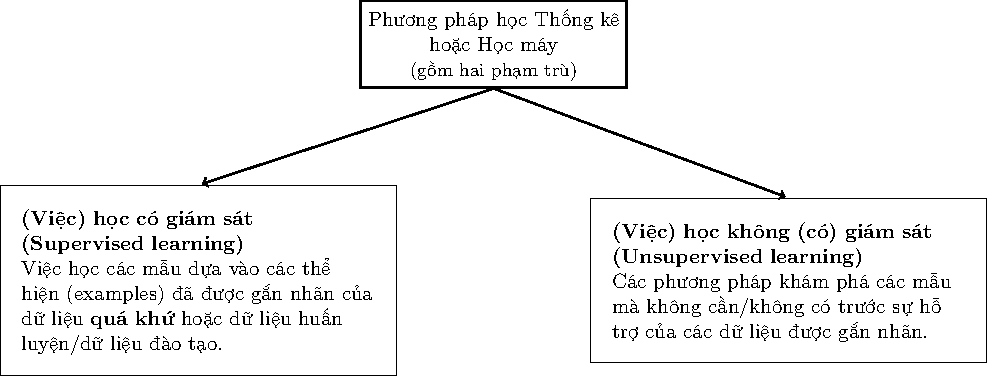
\includegraphics[width=0.85\textwidth]{image/phan_loai_hoc_may.pdf}

	% Thêm chú thích tên hình ở đây (để normal, không in nghiêng)
	\caption{Sơ đồ phân loại các phương pháp học thống kê.}
	\label{fig:phan_loai_hoc_may}
\end{figure}

%================1.1.2
\subsection{Tổng quan về việc học có giám sát}

Các phương pháp học có giám sát có các thành phần chung là:
\begin{itemize} [label=--]
	\item Tập biến đầu vào (Input variables): các thuật ngữ hiện đại được sử dụng trong lĩnh vực học máy (Machine Learning - ML)| Các đặc trưng (features) trong thống kê.
	\item Tập biến đầu ra (Output variables): được tính toán dựa vào quy luật đặt trên tập biến đầu vào. Các biến đầu ra còn được gọi là biến đáp ứng (responses).
\end{itemize}
Một số phương pháp thuộc phạm trù học có giám sát: Hồi quy logistic, Hồi quy tuyến tính,  K-NN (K lân cận gần nhất | K-Nearest Neighbors), LDA (Linear Discriminant Analysis), SVM (Support Vector Machine),...

Một số ứng dụng của phương pháp học có giám sát: 
\begin{itemize} [label=--]
	\item Dự đoán dựa trên hồ sơ nhân khẩu học, chế độ ăn uống, dữ liệu lâm sàng trước đó về khả năng một người có thể mắc bệnh tim (Phạm trù y sinh).
	\item Dự đoán giá một số loại cổ phiếu trong khoảng \textit{t} tháng từ thời điểm hiện tại dựa vào các số đo hiệu suất hoạt động của công ty và dữ liệu kinh tế liên quan (Phạm trù thị trường chứng khoán, cổ phiếu).
	\item Nhận dạng mẫu, chẳng hạn: nhận dạng chữ số, trong một mã nén (zipcode), chữ viết tay từ một ảnh số (Phạm trù chữ ký số, thương mại điện tử).  
\end{itemize}
Ta xét bài toán học theo quan điểm là bài toán tìm mối quan hệ | sự phụ thuộc mong muốn bằng việc sử dụng một tập hữu hạn các đối tượng quan sát (|dữ liệu được quan sát)
\begin{figure}[H]
	\centering
	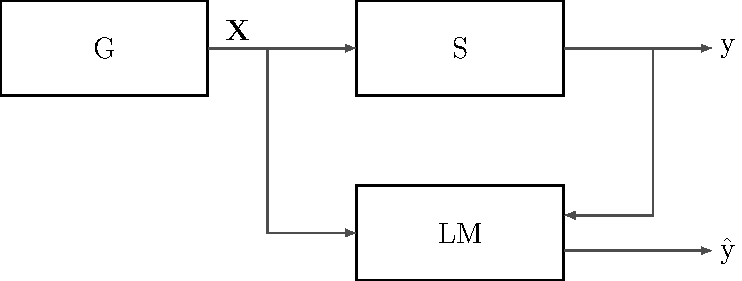
\includegraphics{image/mo_hinh_hoc_may.pdf}
	
	% Thêm chú thích tên hình ở đây (để normal, không in nghiêng)
	\caption{Mô hình toán học máy học.}
	\label{fig:mo_hinh_hoc_may}
\end{figure}
Mô hình chung của việc học từ ví dụ được mô tả ở hình trên như sau:
\begin{enumerate}
	\item[$(i)$] \textbf{Bộ sinh các giá trị của vectơ ngẫu nhiên} $(G)$ (\textit{Generator}): $\bm{x} \in \mathbb{R}^d$ được lấy (một cách) độc lập từ một hàm phân phối xác suất cố định nhưng không biết $F(\bm{x})$.
	\item[$(ii)$] \textbf{Bộ ( | người) giám sát} $(S)$ (\textit{Supervisor}): (mà) trả một giá trị ra (output) $y$ cho mỗi (vectơ) giá trị vào (input) $\bm{x}$, theo một phân phối điều kiện $F(y|\bm{x})$ cũng cố định nhưng không biết.
	\item[$(iii)$] \textbf{Một máy học} $(LM)$ (\textit{learning machine}) có khả năng thực hiện | thực thi tập các hàm $\{f(\bm{x}, \alpha)\}_{\alpha \in \Lambda}$, ở đây $\Lambda$ là một tập các tham số.
\end{enumerate}
Bài toán học là việc chọn, từ tập hợp các hàm $f(\bm{x}, \alpha)$ ($\alpha \in \Lambda$) đã cho, một hàm xấp xỉ tốt nhất cho đáp ứng của (bộ) giám sát. Sự lựa chọn hàm mong muốn là dựa trên một tập dữ liệu huấn luyện gồm $n$ quan sát được lấy một cách độc lập và chung phân phối (i.i.d. -- independent and identically distributed) $F(\bm{x},y) = F(\bm{x}) \cdot F(y|\bm{x})$
\begin{equation}
	(\bm{x}_1, y_1), (\bm{x}_2, y_2), \dots, (\bm{x}_n, y_n).
	\label{eq:1.1}
\end{equation}
Trong suốt quá trình, máy học theo dõi ``kiểu'' mẫu từ các cặp $(\bm{x}, y)$ (tập dữ liệu huấn luyện | tập dữ liệu đào tạo - \textit{the training set}). Sau quá trình đào tạo, máy phải trả về được giá trị $\hat{y}$ cho bất kỳ giá trị vào $\bm{x}$. Mục tiêu là giá trị $\hat{y}$ trả về ``gần'' (| xấp xỉ) với giá trị đáp ứng $y$ của bộ giám sát.

Mức độ tổn thất | mức độ chênh lệch giữa đáp ứng $y$ của bộ giám sát và đáp ứng $f(\bm{x}, \alpha)$ được cung cấp bởi máy học tương ứng với một giá trị vào $\bm{x}$ được ký hiệu là $L(y, f(\bm{x}, \alpha))$. Hàm $L(y, f(\bm{x}, \alpha))$ được gọi là \textbf{hàm tổn thất} (\textit{the loss functional}).

Khi đó, hàm rủi ro (the risk function), ký hiệu $R(\alpha)$, chính là tổn thất trung bình xác định bởi
\begin{equation}
	R(\alpha) = E[L(Y, f(X, \alpha))] = \int L(y, f(\bm{x}, \alpha)) dF(\bm{x}, y).
\end{equation}

$\rightarrow$ \textit{\textbf{Mục đích:}} Tìm hàm $f(\bm{x}, \alpha_0)$ ($\alpha_0 \in \Lambda$) mà cực tiểu $R(\alpha)$ (trên lớp hàm $\{f(\bm{x}, \alpha)\}_{\alpha \in \Lambda}$) trong ngữ cảnh: ta không biết hàm phân phối đồng thời $F(\bm{x}, y)$ và chỉ có sẵn thông tin mẫu được lấy từ nó (tập dữ liệu huấn luyện (\ref{eq:1.1})).

%=============1.1.3

\subsection{Bài toán phân loại mẫu}

% \subsubsection{Khái niệm về mẫu và nhận dạng mẫu thống kê}
Trong thống kê nhiều chiều, bài toán phân loại mẫu thống kê nhằm xác định một đối tượng quan sát thuộc về lớp hay quần thể nào dựa trên các đặc trưng đo được của nó. Giả sử có tập dữ liệu
\begin{equation*}
	\bm{x} = \{\bm{x}_1, \bm{x}_2, \dots, \bm{x}_n\}
\end{equation*}
Trong đó mỗi mẫu $\bm{x}_i$ được biểu diễn bởi $M$ biến đặc trưng. Tập dữ liệu được chia thành $k$ lớp
\begin{equation*}
	\bm{x} = \{C_1, C_2, \dots, C_k\}
\end{equation*}
với $C_j$ là lớp thứ $j$, $n_j$ là số mẫu thuộc lớp đó và
\begin{equation*}
	N=\sum_{j=1}^{k}n_j.
\end{equation*}
\hspace*{0.5cm}Mục tiêu của bài toán phân loại là xây dựng một quy tắc quyết định để khi có một mẫu mới, ta có thể gán mẫu đó vào lớp phù hợp nhất. Trong bối cảnh học có giám sát, nhãn lớp của các mẫu huấn luyện đã biết trước, nhờ đó có thể khai thác thông tin về cấu trúc giữa các lớp để xây dựng bộ phân loại. Đây là một phương pháp giảm chiều có giám sát, trong đó nhãn lớp được sử dụng để tìm ra không gian biểu diễn mới giúp tăng khả năng tách biệt giữa các lớp.
\begin{itemize}
	\item \textbf{Mẫu (Pattern):} Đứng ở góc độ toán học, một ``mẫu'' được biểu diễn như một vectơ đặc trưng $\mathbf{X} = \bm{x} \in \mathbb{R}^d$, đại diện cho các thuộc tính định lượng được trích xuất từ một đối tượng quan sát.
	
	\item \textbf{Nhận dạng (Recognition):} Là quá trình ánh xạ một mẫu $\bm{x}$ vào một trong các lớp (class) $\mathbf{y}$ thuộc một tập hợp rời rạc cho trước. Trong ngôn ngữ học máy, đây chính là bài toán Phân loại (Classification).
	
	\item \textbf{Nhận dạng mẫu thống kê (Statistical Pattern Recognition):} Phương pháp này xem xét sự biến thiên của các mẫu là ngẫu nhiên và giải quyết bài toán nhận dạng bằng cách tìm mối quan hệ bản chất giữa không gian đặc trưng $\mathcal{X}$ và không gian nhãn $\mathcal{Y}$ thông qua lý thuyết xác suất.
\end{itemize}
\hspace*{0.5cm}Đối với bài toán phân loại mẫu thống kê bằng hồi quy tuyến tính và hồi quy logistic, tư tưởng cốt lõi là xây dựng các hàm quyết định (hàm dự báo hoặc ranh giới phân lớp) từ dữ liệu thực nghiệm nhằm thiết lập mối liên hệ giữa các biến đặc trưng đầu vào và nhãn lớp đầu ra. Trong khi hồi quy tuyến tính tiếp cận bài toán phân loại dưới dạng ước lượng trực tiếp giá trị của nhãn lớp bằng cách tối ưu hóa sai số bình phương trung bình, thì hồi quy logistic lại tập trung mô hình hóa xác suất có điều kiện thuộc về các lớp thông qua hàm sigmoid (logistic). Vì vậy, bài toán phân loại mẫu thống kê gắn chặt với việc tối ưu hóa các tham số để thiết lập ranh giới phân lớp tối ưu trong không gian đặc trưng.
% Đối với bài toán LDA, tư tưởng cốt lõi không chỉ là giảm số chiều của dữ liệu mà còn là tìm một phép chiếu tuyến tính sao cho các lớp sau khi chiếu trở nên ``dễ phân biệt'' nhất. Vì vậy, bài toán phân loại mẫu trong LDA gắn chặt với việc đánh giá mức độ phân tán của dữ liệu trong từng lớp và mức độ tách biệt giữa các lớp.



% \subsubsection{ Tiêu chuẩn tối ưu: kỳ vọng có điều kiện}
\hspace*{0.5cm}Như đã trình bày ở phần trước, mục tiêu của quá trình học là cực tiểu hóa hàm rủi ro $R(\alpha)$. Trong bối cảnh bài toán không có chi phí phạt đặc thù cho từng loại sai sót, hàm tổn thất tự nhiên và phổ biến nhất được sử dụng là tổn thất bình phương (Squared Loss)
\begin{equation*}
	L(y, f(\bm{x}, \alpha)) = (y - f(\bm{x}, \alpha))^2
\end{equation*}
Khi đó, hàm rủi ro trở thành sai số bình phương trung bình (Mean Squared Error - MSE)
\begin{equation*}
	R(\alpha) = E\left[(Y - f(\bm{X}, \alpha))^2\right]
\end{equation*}
Trước khi đi tìm tham số $\alpha$ cụ thể, ta xét bài toán tối ưu ở mức độ tổng quát hơn: Giả sử ta không bị giới hạn bởi năng lực của máy học, tức là ta có thể tìm kiếm tự do trong một không gian toàn bộ các phiếm hàm đo được $\mathcal{F}$. Ta cần tìm phiếm hàm $\phi(x) \in \mathcal{F}$ sao cho rủi ro là nhỏ nhất
\begin{equation*}
	\phi(x) = \arg\min_{h \in \mathcal{F}} E\left[(Y - h(\bm{X}))^2\right]
\end{equation*}
Bằng cách thêm bớt thành phần $E(Y|\bm{X})$ — là kỳ vọng có điều kiện của đáp ứng $Y$ từ bộ giám sát cho trước giá trị vào $\bm{X}$ — ta khai triển hàm mục tiêu
\begin{align*}
	E\left[Y - h(\bm{X})\right]^2 &= E\left[Y - E(Y|\bm{X}) + E(Y|\bm{X}) - h(\bm{X})\right]^2 \nonumber \\
	&= E\left[Y - E(Y|\bm{X})\right]^2 + E\left[E(Y|\bm{X}) - h(\bm{X})\right]^2 \nonumber \\
	& \quad + 2E\left[\left(Y - E(Y|\bm{X})\right)\left(E(Y|\bm{X}) - h(\bm{X})\right)\right]
\end{align*}
Trong đó,
\begin{equation*}
	E\left[\left(Y - E(Y|\bm{X})\right)\left(E(Y|\bm{X}) - h(\bm{X})\right)\right] = E\left\{ E\left[ \left(Y - E(Y|\bm{X})\right)\left(E(Y|\bm{X}) - h(\bm{X})\right) \mid \bm{X} \right] \right\}
\end{equation*}
Vì $E(Y|\bm{X})$ và $h(\bm{X})$ là các đại lượng đo được theo $\bm{X}$, nên theo tính chất kỳ vọng có điều kiện
\begin{equation*}
	E\left\{ E\left[ \left(Y - E(Y|\bm{X})\right)\left(E(Y|\bm{X}) - h(\bm{X})\right) \mid \bm{X} \right] \right\} = E\left\{ \left(E(Y|\bm{X}) - h(\bm{X})\right) \underbrace{E\left[ Y - E(Y|\bm{X}) \mid \bm{X} \right]}_{(*)} \right\}
\end{equation*}
Ta xét riêng thành phần $(*)$
\begin{equation*}
	E\left[ Y - E(Y|\bm{X}) \mid \bm{X} \right] = E(Y|\bm{X}) - E\left[ E(Y|\bm{X}) \mid \bm{X} \right] = E(Y|\bm{X}) - E(Y|\bm{X}) = 0
\end{equation*}
Do đó,
\begin{equation*}
	R(h) = E\left[Y - E(Y|\bm{X})\right]^2 + E\left[E(Y|\bm{X}) - h(\bm{X})\right]^2\geq E\left[Y - E(Y|\bm{X})\right]^2
\end{equation*}
Từ đó suy ra, phiếm hàm xấp xỉ tốt nhất chính là
\begin{equation*}
	\phi(\bm{X}) = E(Y \mid \bm{X})
\end{equation*}
Nói cách khác, hàm dự báo tốt nhất về mặt lý thuyết chính là kỳ vọng có điều kiện của biến đáp ứng theo nhóm biến quan trắc từ bộ giám sát.

\hspace*{0.5cm}Mặc dù đã chứng minh được kết quả tối ưu lý tưởng $\phi(\bm{X}) = E(Y|\bm{X})$, ta lại vấp phải giới hạn thực tế: ta không biết phân phối đồng thời $F(\bm{x},y)$, do đó không thể xác định được dạng giải tích của $E(Y|\bm{X})$. Đây chính là lúc \textbf{năng lực của máy học (Learning Machine)} được thể hiện. Thay vì mò mẫm trong không gian $\mathcal{F}$ rộng lớn, máy học thực thi bài toán bằng cách \textbf{tham số hóa} (parameterization). Ta giả định rằng tồn tại một bộ tham số tối ưu $\alpha_0 \in \Lambda$ sao cho hàm $f(\bm{X}, \alpha_0)$ là một xấp xỉ đủ tốt cho $\phi(\bm{X})$ nghĩa là
\begin{equation*}
	E(Y|X) \approx f(\bm{X}, \alpha_0)
\end{equation*}

Khi đó, bài toán học không còn là tìm một hàm $\phi$ trừu tượng, mà được quy về việc sử dụng tập dữ liệu huấn luyện (\ref{eq:1.1}) để ước lượng bộ tham số $\hat{\alpha} \in \Lambda$.










%================1.2
\section{Mẫu từ vector đặc trưng nhiều chiều của quần thể}


Như đã đề cập ở phần trên, bài toán phân loại mẫu thống kê đề cập đến mẫu ngẫu nhiên trong một quần thể. Cho điểm (vectơ) ngẫu nhiên $d$ chiều $\bm{X} = (X_1, X_2, \dots, X_d)^\text{T}$ có hàm phân phối xác suất đồng thời $F(\bm{x} \mid \mu, \Sigma)$ không được biết rõ. Dãy các điểm ngẫu nhiên $d$ chiều $\bm{X}_1, \bm{X}_2, \dots, \bm{X}_n$ gọi là một mẫu ngẫu nhiên (đơn giản) cỡ $n$ lấy từ điểm ngẫu nhiên $\bm{X}$ nếu như các $\bm{X}_k$ ($k = 1, 2, \dots, n$) là độc lập và có chung phân phối $F(\bm{x} \mid \mu, \Sigma)$ với $\bm{X}$. Mẫu ngẫu nhiên này có thể được biểu diễn dưới dạng ma trận dữ liệu như sau
\begin{equation*}
	\mathbf{X} = 
	\begin{pmatrix}
		\bm{X}_1^\text{T} \\
		\bm{X}_2^\text{T} \\
		\vdots \\
		\bm{X}_n^\text{T}
	\end{pmatrix}
	=
	\begin{pmatrix}
		X_{11} & X_{12} & \dots & X_{1d} \\
		X_{21} & X_{22} & \dots & X_{2d} \\
		\vdots & \vdots & \ddots & \vdots \\
		X_{n1} & X_{n2} & \dots & X_{nd}
	\end{pmatrix}
\end{equation*} ở đây $\bm{X}_i \in \mathbb{R}^d$, $\bm{X}_i = (X_{i1}, X_{i2}, \dots, X_{id})^\text{T}$, $i = 1, \dots, n$. Giá trị thể hiện hay còn gọi là giá trị được quan sát, được ghi nhận của một mẫu ngẫu nhiên sẽ được viết chữ nhỏ như thông thường, chẳng hạn
\begin{equation*}
	\bm{x} = (\bm{x}_1, \bm{x}_2, \dots, \bm{x}_n)^\text{T} = 
	\begin{pmatrix}
		x_{11} & x_{12} & \dots & x_{1d} \\
		x_{21} & x_{22} & \dots & x_{2d} \\
		\vdots & \vdots & \ddots & \vdots \\
		x_{n1} & x_{n2} & \dots & x_{nd}
	\end{pmatrix}
\end{equation*} để chỉ cho giá trị được quan sát hoặc ma trận dữ liệu mẫu của mẫu ngẫu nhiên này, trong đó: $\bm{X}_i = \bm{x}_i \equiv (x_{i1}, x_{i2}, \dots, x_{id})^\text{T}$ là giá trị thể hiện của $\bm{X}_i$ (hoặc giá trị quan sát được của $\bm{X}$ ở lần thứ $i$ trong mẫu ($i = 1, 2, \dots, n$)).

Ta cũng có thể trình bày theo dạng bảng dữ liệu thống kê thô (thường sử dụng để mô tả, chẳng hạn, cho dữ liệu đầu vào của một thủ tục phân tích hồi quy) như sau
\begin{table}[H]
\centering
\renewcommand{\arraystretch}{1.2} % Tăng khoảng cách dòng cho dễ nhìn
\begin{tabular}{|c||cccc|}
\hline
\multirow{2}{*}{\makecell{\textnormal{STT}}} & \multicolumn{4}{|c|}{Các dấu hiệu (Các biến)} \\ \cline{2-5} 
 & $X_1$ & $X_2$ & $\dots$ & $X_d$ \\ \hline
\textnormal{1} & $x_{11}$ & $x_{12}$ & $\dots$ & $x_{1d}$ \\
\textnormal{2} & $x_{21}$ & $x_{22}$ & $\dots$ & $x_{2d}$ \\
$\vdots$ & $\vdots$ & $\vdots$ & $\vdots$ & $\vdots$ \\
\textnormal{i} & $x_{i1}$ & $x_{i2}$ & $\dots$ & $x_{id}$ \\
$\vdots$ & $\vdots$ & $\vdots$ & $\vdots$ & $\vdots$ \\
\textnormal{n} & $x_{n1}$ & $x_{n2}$ & $\dots$ & $x_{nd}$ \\ \hline
\end{tabular}
\caption{Bảng dữ liệu thống kê thô của các biến đầu vào}
\label{tab:raw_data}
\end{table}
Trong đó,
\begin{itemize}
	\item Mỗi cột đại diện cho dữ liệu quan sát một biến.
	\item Hàng thứ $i$ đại diện cho giá trị thể hiện của quan sát thứ $i$, ký hiệu là $\bm{x}_i$, ($i = 1, 2, \dots, n$). Trong đó
	\[
	\bm{x}_i = (x_{i1}, x_{i2}, \dots, x_{id})^{\top},
	\]
	và $x_{ij}$ là giá trị quan sát thứ $i$ của biến $X_j$, với $j = 1, 2, \dots, d$.
\end{itemize}




%================1.3
\section{Phân tích tương quan và các moment đặc trưng mẫu}

Trong phân tích dữ liệu đa biến, việc nghiên cứu mối quan hệ giữa các biến và mô tả đặc trưng của mẫu đóng vai trò nền tảng. Thông qua các công cụ thống kê như trung bình và vectơ trung bình, ta có thể tóm tắt xu hướng phân bố của dữ liệu cũng như hỗ trợ cho các phương pháp phân tích nâng cao như phân tích tương quan hay phân lớp.

Cho $\bm{X} = (X_1, X_2, \dots, X_d)^T$ là một điểm ngẫu nhiên $d$ chiều. Xét mẫu ngẫu nhiên cỡ $n$ lấy từ $\bm{X}$, ký hiệu bởi $\bm{x}_1, \bm{x}_2, \dots, \bm{x}_{n}$, với $\bm{x}_i \in \mathbb{R}^d$. Ta quan tâm đến các moment đặc trưng sau đây.

%================1.3.1
\subsection{Các mô-men đặc trưng mẫu}

Cho $\bm{x}_{1}, \bm{x}_{2}, \dots, \bm{x}_{n}$ là mẫu thể hiện cỡ $n$ lấy từ vectơ ngẫu nhiên $d$ chiều $\bm{X} = (\bm{X}_1, \bm{X}_2, \dots, \bm{X}_d)^\top$. Ta quan tâm các moment mẫu đặc trưng sau đây.
\begin{itemize}
	\item Điểm (vectơ) trung bình mẫu (the sample mean vector) là vectơ  $d$ chiều xác định bởi
	\begin{equation}
		\overline{\bm{x}} \equiv \frac{1}{n} \sum_{i=1}^{n} \bm{x}_i = \begin{pmatrix} 
			\overline{x}_1 \\ 
			\overline{x}_2 \\ 
			\vdots \\ 
			\overline{x}_d 
		\end{pmatrix},
	\end{equation}
	trong đó
	\begin{equation}
		\overline{x}_j = \frac{1}{n} \sum_{i=1}^{n} x_{ij}
	\end{equation}
	là trung bình mẫu của quan sát trên biến thứ $j$ ($j = 1, 2, \dots, d$).
\end{itemize}


\begin{itemize}
	\item Ma trận hiệp phương sai mẫu (the sample covariance matrix) được xác định như sau
	\begin{equation}
		S = \frac{1}{n-1} \sum_{i=1}^{n} (\bm{x}_i - \overline{x})(\bm{x}_i - \overline{x})^{\top} = 
		\begin{pmatrix}
			s_{11} & s_{12} & \dots & s_{1d} \\
			s_{21} & s_{22} & \dots & s_{2d} \\
			\vdots & \vdots & \ddots & \vdots \\
			s_{d1} & s_{d2} & \dots & s_{dd}
		\end{pmatrix},
	\end{equation}
	ở đây 
	\begin{equation}
		s_{jk} = \frac{1}{n-1} \sum_{i=1}^{n} (x_{ij} - \overline{x}_j)(x_{ik} - \overline{x}_k)
	\end{equation}
	là hiệp phương sai mẫu của hai biến thứ $j$ và thứ $k$, và 
	\begin{equation}
		s_{jj} = \frac{1}{n-1} \sum_{i=1}^{n} (x_{ij} - \overline{x}_j)^2
	\end{equation}
	là phương sai mẫu của biến thứ $j$.
\end{itemize}

\subsection{Hệ số tương quan mẫu}

Hiệp phương sai cung cấp thông tin về xu hướng biến thiên đồng thời giữa các biến ngẫu nhiên, tuy nhiên đại lượng này phụ thuộc vào thang đo của từng biến nên khó sử dụng để so sánh mức độ liên hệ giữa các cặp biến khác nhau.

Do đó, cần xây dựng một đại lượng chuẩn hóa từ hiệp phương sai, không phụ thuộc vào đơn vị đo, nhằm phản ánh chính xác mức độ và chiều hướng của mối quan hệ tuyến tính giữa các biến. Đại lượng đó chính là hệ số tương quan.

Với $\bm{x}_1, \bm{x}_2, \dots, \bm{x}_n$ là mẫu thể hiện cỡ $n$ được lấy từ vectơ ngẫu nhiên $d$ chiều $\bm{X} = (X_1, X_2, \dots, X_d)^T$, và đặt $X_j^*$ là biến ngẫu nhiên mẫu ứng với biến $X_j$ ($j=\overline{1,d}$), nghĩa là 
\begin{equation*}
	P(X_j^*=x_{ij}) = \frac{1}{n}, \quad \forall i= 1,2,\dots,n
\end{equation*} Khi đó, hệ số tương quan mẫu giữa hai biến thứ $j$ và thứ $k$ (ký hiệu $r_{jk}$) được xác định là hệ số tương quan giữa hai biến $X_j^*$ và $X_k^*$

\begin{equation}
	\begin{aligned}
		r_{jk}=\rho_{X_j^*, X_k^*} &= \frac{\text{cov}(X_j^*, X_k^*)}{\sqrt{D(X_j^*)D(X_k^*)}} \\
		&= \frac{s_{jk}}{\sqrt{s_{jj} s_{kk}}} = \frac{\sum_{i=1}^n (x_{ij} - \overline{x}_j)(x_{ik} - \overline{x}_k)}{\sqrt{\sum_{i=1}^n (x_{ij} - \overline{x}_j)^2} \sqrt{\sum_{i=1}^n (x_{ik} - \overline{x}_k)^2}} .
	\end{aligned}
	\label{eq:1.8}
\end{equation}

\hspace*{0.5cm}Để thấy được ý nghĩa hình học của hệ số tương quan mẫu $r_{jk}$, ta xét một không gian con đặc biệt được sinh bởi vectơ toàn phần tử bằng 1. Không gian này đóng vai trò quan trọng trong việc xác định hướng chiếu và diễn giải ý nghĩa của các phép biến đổi tuyến tính.

Xét không gian vectơ $\mathbb{R}^n$ với tích vô hướng Euclid của hai vectơ $\bm{x} = (x_1, x_2,\dots,x_n)^T$, $\bm{y} = (y_1, y_2,\dots,y_n)^T$ được xác định bởi công thức
$$
\langle \bm{x}, \bm{y} \rangle = \sum_{i=1}^n x_i y_i.
$$
Với tích vô hướng trên, độ dài (chuẩn) của một vectơ $\bm{x} \in \mathbb{R}^n$ được ký hiệu và cho bởi
$$
\|\bm{x}\| = \sqrt{\langle \bm{x}, \bm{x} \rangle} = \sqrt{\sum_{i=1}^n x_i^2}.
$$
Đồng thời, cosin của góc giữa hai vectơ $\bm{x}, \bm{y}$ cũng được xác định như sau
$$
\cos(\bm{x}, \bm{y}) = \frac{\langle \bm{x}, \bm{y} \rangle}{\|\bm{x}\| \|\bm{y}\|}.
$$
Và $\bm{x}$, $\bm{y}$ được gọi là vuông góc với nhau, ký hiệu $\bm{x} \perp \bm{y}$, nếu như 
$$
\cos(\bm{x}, \bm{y}) = 0 \iff \langle \bm{x}, \bm{y} \rangle = 0.
$$
Khi đó, ứng với $\mathbf{1} = (1, 1,\dots,1)^T \in \mathbb{R}^n$, không gian con sinh bởi vectơ này được cho bởi
$$
\langle \mathbf{1} \rangle = \{\alpha \mathbf{1} \mid \alpha \in \mathbb{R}\}.
$$

Không gian $\langle \mathbf{1} \rangle$ biểu diễn đường phân giác thứ nhất hay đường phân giác chính trong hệ trục $\{e_i\}_{i=\overline{1,n}}$, là hệ trục vuông góc chính tắc của $\mathbb{R}^n$. Nói cách khác, vectơ $\mathbf{1}$ tạo với các vectơ đơn vị $e_i$ những góc bằng nhau, do đó $\langle \mathbf{1} \rangle$ chính là không gian sinh bởi vectơ chỉ phương của đường chéo chính trong $\mathbb{R}^n$. Từ cách diễn giải hình học trên, ta có thể xét phép chiếu trực giao của một vectơ bất kỳ lên không gian con $\langle \mathbf{1} \rangle$. Cụ thể, hình chiếu trực giao của vectơ $x_j^*$ lên $\langle \mathbf{1} \rangle$, kí hiệu $\text{proj}_{\mathbf{1}} x_j^*$, với $\bm{x}_j^* = (x_{1j},x_{2j},\dots,x_{nj})^T$ được cho bởi hình sau

\begin{figure}[H]
	\centering
	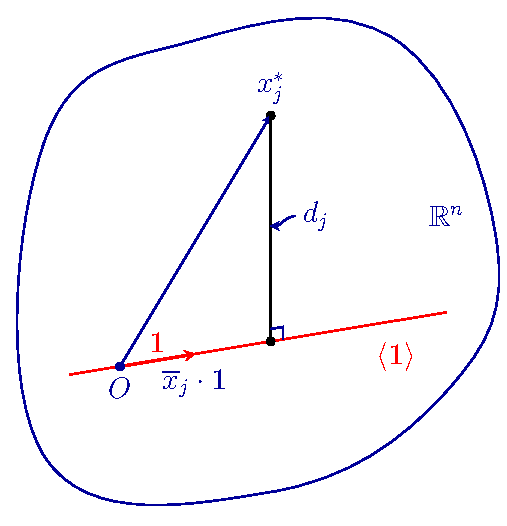
\includegraphics{image/phep_chieu_2.pdf}
	\caption{Hình chiếu trực giao của $\bm{x}_j^*$ lên $\langle \mathbf{1} \rangle$}
	\label{fig:phep_chieu_2}
\end{figure}

Ta chỉ ra $\text{proj}_{\mathbf{1}} \bm{x}_j^* = \overline{x}_j \cdot \mathbf{1}$. Thực vậy, ta có
$$
\begin{aligned}
	\text{proj}_{\mathbf{1}} \bm{x}_j^* 
	&= \|\bm{x}_j^*\| \cos(\bm{x}_j^*, \mathbf{1}) \cdot \frac{\mathbf{1}}{\|\mathbf{1}\|} \\
	&= \|\bm{x}_j^*\| \frac{\langle \bm{x}_j^*, \mathbf{1} \rangle}{\|\bm{x}_j^*\| \|\mathbf{1}\|} \cdot \frac{\mathbf{1}}{\|\mathbf{1}\|} \\
	&= \frac{\langle \bm{x}_j^*, \mathbf{1} \rangle}{\|\mathbf{1}\|^2} \cdot \mathbf{1} \\
	&= \left( \frac{1}{n} \sum_{i=1}^n x_{ij} \right) \cdot \mathbf{1} \\
	&= \overline{x}_j \cdot \mathbf{1}.
\end{aligned}
$$ Vectơ $d_j=\bm{x}_j^*-\overline{x}_j\cdot \mathbf{1} \quad (j =1,2,\dots,d)$ được gọi là vectơ độ lệch của $x_j^*$ đối với $\langle\mathbf{1}\rangle$.

Bước tiếp theo, với hai vectơ $x_j^*$ và $x_k^*$, ta thực hiện phép chiếu (trực giao) của các vectơ này lên $\langle\mathbf{1}\rangle$. (Xem hình \ref{fig:hilbert_3})

\begin{figure}[H]
	\centering
	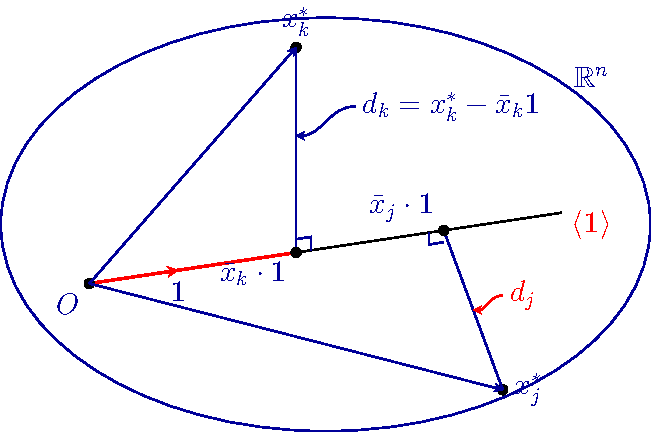
\includegraphics{image/hilbert_3.pdf}
	\caption{Hình chiếu trực giao của hai vectơ $\bm{x}_j^*$, $\bm{x}_k^*$ lên $\langle\mathbf{1}\rangle$}
	\label{fig:hilbert_3}
\end{figure} Đặt, 
$$
\begin{aligned}
	S_j &\equiv \langle \mathbf{1} ,\bm{x}_j^*\rangle = \{\alpha \mathbf{1}+\beta \bm{x}_j^* \mid \alpha,\beta \in \mathbb{R} \}; \\
	S_k &\equiv \langle \mathbf{1}, \bm{x}_k^* \rangle = \{\alpha \mathbf{1}+\beta \bm{x}_k^* \mid \alpha,\beta \in \mathbb{R} \}
\end{aligned}
$$ lần lượt là các mặt phẳng (không gian con) được sinh ra bởi vectơ $\mathbf{1}$ và vectơ $\mathbf{1}$ và một trong hai vectơ $\bm{x}_j^*$ hoặc $\bm{x}_k^*$. Khi đó, cosin giữa góc tạo bởi hai mặt phẳng trên được xác định như sau
$$
\begin{aligned}
	\cos(S_j, S_k) = \cos(\bm{d}_j, \bm{d}_k) \\
	&= \frac{\langle \bm{d}_j, \bm{d}_k \rangle}{\|\bm{d}_j\| \|\bm{d}_k\|} \\
	&= \frac{\sum_{i=1}^n (x_{ij}-\overline{x}_j)(x_{ik}-\overline{x}_k)}{\sqrt{\sum_{i=1}^n(x_{ij}-\overline{x}_j)^2}\sqrt{\sum_{i=1}^n(x_{ik}-\overline{x}_k)^2}} \\
	&= r_{jk}.
\end{aligned}
$$ Ở đây, $d_j = \bm{x}_j^* - \overline{x}_j \cdot \mathbf{1}$ và $d_k = \bm{x}_k^* - \overline{x}_k \cdot \mathbf{1}$ là các vectơ độ lệch của $\bm{x}_j^*$ và $\bm{x}_k^*$ đối với $\langle\mathbf{1}\rangle$.
Bằng việc sử dụng bất đẳng thức Cauchy-Schwarz cho tích vô hướng, có thể thấy 
$$
\begin{aligned}
	|r_{jk}| = 1 &\iff \bm{d}_j = b \bm{d}_k \quad (b \in \mathbb{R}) \\
	&\iff \bm{x}_j^* - \overline{x}_j \mathbf{1} = b(\bm{x}_k^* - \overline{x}_k \mathbf{1}) \\
	&\iff \bm{x}_j^* = b\bm{x}_k^* + a \mathbf{1} \quad (a = \overline{x}_j - b\overline{x}_k).
\end{aligned}
$$ Tức, $\bm{x}_j^* \in S_k$ hay $S_j \equiv S_k$. Điều này nghĩa là có một liên hệ tuyến tính thực sự giữa hai vectơ $\bm{x}_j^*$ và $\bm{x}_k^*$. Khi $r_{jk}=-1$ thì sự phụ thuộc tuyến tính của các giá trị $x_{ij}$ và $x_{ik}$ là nghịch biến và $r_{jk}=1$ thì sự phụ thuộc này là đồng biến.

Ngược lại, khi $r_{jk}=0$, tức $\bm{d}_k \perp \bm{d}_j$ (hay $S_j \perp S_k$) thì mối liên hệ tuyến tính giữa $\bm{d}_j$ và $\bm{d}_k$ là kém hiệu quả nhất. Lúc này, ta nói $\bm{x}_j^*$ và $\bm{x}_k^*$ là không có tương quan tuyến tính với nhau. 

Đồ thị đám mây điểm biểu diễn mức độ tương quan (tuyến tính) của hai vectơ $\bm{x}_j^*$ và $\bm{x}_k^*$ được cho trong hình sau

\begin{figure}[H]
	\centering
	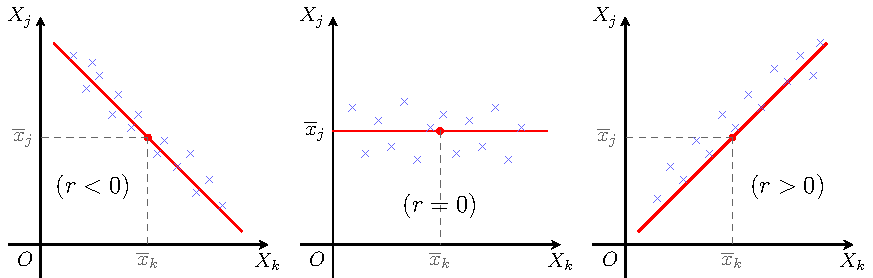
\includegraphics{image/tuongquan.pdf}
	\caption{Đồ thị đám mây điểm biểu diễn mức độ tương quan của hai vectơ $\bm{x}_j^*$ và $\bm{x}_k^*$}
	\label{fig:tuongquan}
\end{figure}


\subsection{Ma trận tương quan mẫu và hệ số tải}
Từ dữ liệu thống kê cỡ $n$ được lấy từ vectơ ngẫu nhiên $d$ chiều $\bm{X} = (X_1,\dots,X_d)^T$, cho trong bảng \ref{tab:raw_data}, ta định nghĩa ma trận tương quan mẫu $\mathbf{r}$ ứng với bộ dữ liệu trên được xác định như sau
\begin{equation}
	\bm{r}= 
	\begin{bmatrix}
		1 & r_{12} & \cdots & r_{1d} \\
		r_{21} & 1 & \cdots & r_{2d} \\
		\vdots & \vdots & \ddots & \vdots \\
		r_{d1} & r_{d2} & \cdots & 1
	\end{bmatrix}, 
	\label{eq:1.9}
\end{equation} với $r_{jk}$ là hệ số tương quan mẫu giữa biến thứ $j$ và biến thứ $k$ được cho trong \ref{eq:1.8} $(j,k = 1,2,\dots,d)$. Do $r_{jk}=r_{kj}$ nên ma trận $\bm{r}$ là đối xứng. Hơn nữa, do tính chất của tương quan mẫu, ta có $r_{jk}=r_{k,j}$ với mọi $k,j=1,2,\dots,d$ nên $\bm{r}$ là ma trận đối xứng. Lưu ý rằng, nếu đặt $\bm{d}_j^*$ ($j=1,2,\dots,d$) là vectơ chuẩn hóa của $\bm{d}_j$, nghĩa là
\begin{equation*}
	\bm{d}_j^*=\frac{\bm{d}_j}{\|\bm{d}_j\|},
\end{equation*} thì $\|\bm{d}_j^*\|=1$ và
\begin{equation}
	\begin{aligned}
		r_{jk} &= \cos(\bm{d}_j, \bm{d}_k) = \frac{\langle \bm{d}_j, \bm{d}_k \rangle}{\|\bm{d}_j\| \|\bm{d}_k\|} \\
		&= \left\langle \frac{\bm{d}_j}{\|\bm{d}_j\|}, \frac{\bm{d}_k}{\|\bm{d}_k\|} \right\rangle \\
		&= \cos(\bm{d}_j^*, \bm{d}_k^*). 
	\end{aligned}
	\label{eq:1.10}
\end{equation}
Một điểm cần chú ý ở đây, khi áp dụng các công cụ thống kê vào thực tế, thông thường thang đo thứ nguyên của các biến $X_j$, $(j=1,2,\dots,d)$ là khác nhau. Do vậy để phản ánh chính xác mối tương quan giữa biến $X_j$ và tổng thể trên dữ liệu mẫu ta cần sử dụng đến hệ số tải (loading factor) cho $X_j$. Đặt,
\begin{align*}
	F &= \bm{d}_1^* + \bm{d}_2^* + \dots + \bm{d}_d^* \\
	&= \sum_{j=1}^d \bm{d}_j^*
\end{align*} là vectơ tổng hợp lực của $d$ vectơ $\bm{d}_j^*$. Hệ số tải ứng với biến $X_j$ (trên dữ liệu mẫu) được cho bởi cosin của góc giữa vectơ $\bm{d}_j^*$ với vectơ tổng hợp lực $F$. Tức là, với $\theta_j = \widehat{(\bm{d}_j^*, F)}$
\begin{equation*}
	\cos(\theta_j) = \cos(\bm{d}_j^*, F).
\end{equation*}
Từ ma trận tương quan mẫu được cho trong \ref{eq:1.9}, hệ số tải ứng với biến $X_j$ được xác định như sau
\begin{equation*}
	\cos(\theta_j) = \frac{\text{Tổng cột | hàng } j \text{ của ma trận } \bm{r}}{\sqrt{\text{Tổng các số hạng của ma trận } \bm{r}}}.
\end{equation*} Thực vậy,
\begin{align*}
	\cos(\theta_j) &= \cos(\bm{d}_j^*, F) \\
	&= \frac{\langle \bm{d}_j^*, F \rangle}{\|\bm{d}_j^*\| \|F\|}.
\end{align*} Ta có,
\begin{align*}
	\langle \bm{d}_j^*, F \rangle &= \left\langle d_j^*, \sum_{k=1}^d d_k^* \right\rangle \\
	&= \sum_{k=1}^d \langle d_j^*, d_k^* \rangle \\
	&= \sum_{k=1}^d r_{jk} \quad \text{(theo~\eqref{eq:1.10})}\\
	&= \text{Tổng cột | hàng $j$ của ma trận $\bm{r}$}
\end{align*} Hơn nữa,
\begin{align*}
	\|F\|^2 &= \langle \sum_{j=1}^d d_j^*,F \rangle\\
	&= \langle \sum_{j=1}^d d_j^*,\sum_{k=1}^d d_k^* \rangle\\
	&= \sum_{j=1}^d\langle d_j^*, F \rangle\\
	&= \text{Tổng các số hạng của ma trận $r$}.
\end{align*} Vì thế,
\begin{equation*}
	\cos(\theta_j) = \frac{\text{Tổng cột | hàng $j$ của ma trận $\bm{r}$}}{\sqrt{\text{Tổng các số hạng của ma trận $\bm{r}$}}}.
\end{equation*} Trực quan hóa hệ số tải trong trường hợp $d=2$ được cho bởi hình sau
\begin{figure}[H]
	\centering
	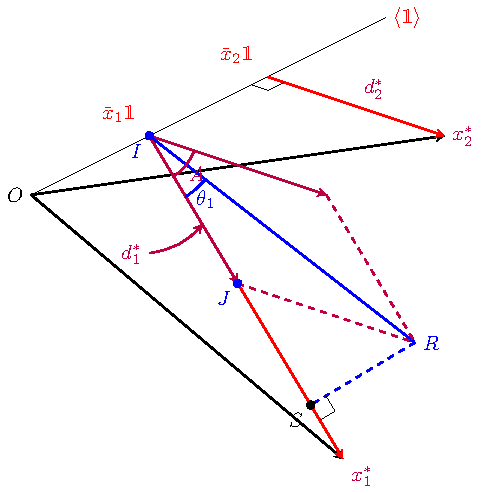
\includegraphics[width=0.7\linewidth]{image/vector_loading_x1.pdf}
	\caption{Minh họa hình học cho hệ số tải}
	\label{fig:vector_angles}
\end{figure}
Để minh họa cho cách xác định hệ số tải, ta xét ví dụ sau

\textbf{Trường hợp} $d = 3$. Xét trường hợp có ba biến $X_1, X_2, X_3$. Khi đó, ta có ba vectơ sai lệch chuẩn hoá
\[
d_1^*, \quad d_2^*, \quad d_3^*.
\]
Gọi $R$ là vectơ tổng hợp của ba vectơ này
\[
R = d_1^* + d_2^* + d_3^*.
\]
Hệ số tải của biến $X_i$ trên vectơ tổng hợp $R$ được xác định bởi cosin của góc giữa $d_i^*$ và $R$
\[
a_i = \cos \theta_i = \cos(d_i^*, R).
\]
Theo định nghĩa cosin giữa hai vectơ
\[
\cos \theta_i = \frac{d_i^{*T} R}{\|d_i^*\| \|R\|}.
\]
Vì $d_i^*$ đã được chuẩn hoá nên
\[
\|d_i^*\| = 1.
\]
Do đó
\[
a_i = \cos \theta_i = \frac{d_i^{*T} R}{\|R\|}.
\]
Với $R = d_1^* + d_2^* + d_3^*$, ta có
\[
a_1 = \frac{1 + r_{12} + r_{13}}{\|R\|},
\]
\[
a_2 = \frac{r_{21} + 1 + r_{23}}{\|R\|},
\]
\[
a_3 = \frac{r_{31} + r_{32} + 1}{\|R\|}.
\]
Như vậy, tử số của mỗi hệ số tải chính là tổng các phần tử trên hàng tương ứng của ma trận tương quan. Tổng quát, với $d$ biến
\[
a_i = \frac{\sum_{j=1}^d r_{ij}}{\|R\|}.
\]
Trong đó,
\[
R = \sum_{j=1}^d d_j^*.
\]
Độ dài của vectơ tổng hợp $R$ được xác định bởi
\[
\|R\|^2 = \sum_{i=1}^d \sum_{j=1}^d r_{ij}.
\]
Do đó
\[
\|R\| = \sqrt{\sum_{i=1}^d \sum_{j=1}^d r_{ij}}.
\]
Suy ra công thức tổng quát của hệ số tải là
\[
\boxed{ a_i = \cos \theta_i = \frac{\sum_{j=1}^d r_{ij}}{\sqrt{\sum_{i=1}^d \sum_{j=1}^d r_{ij}}} }.
\]
Áp dụng với ma trận tương quan đã cho
\[
R = \begin{pmatrix}
	1 & 0,9659 & 0,2588 \\
	0,9659 & 1 & 0,5000 \\
	0,2588 & 0,5000 & 1
\end{pmatrix},
\]
ta có
\[
r_{12} = 0,9659, \qquad r_{13} = 0,2588, \qquad r_{23} = 0,5000.
\]
Tổng tất cả các phần tử trong ma trận tương quan là
\[
\sum_{i=1}^3 \sum_{j=1}^3 r_{ij} = 3 + 2(r_{12} + r_{13} + r_{23}).
\]
Thay số
\[
\sum_{i=1}^3 \sum_{j=1}^3 r_{ij} = 3 + 2(0,9659 + 0,2588 + 0,5000) = 6,4494.
\]
Do đó
\[
\|R\| = \sqrt{6,4494} \approx 2,5396.
\]
Hệ số tải của từng biến là
\[
a_1 = \frac{1 + 0,9659 + 0,2588}{\sqrt{6,4494}} = \frac{2,2247}{2,5396} \approx 0,8760,
\]
\[
a_2 = \frac{0,9659 + 1 + 0,5000}{\sqrt{6,4494}} = \frac{2,4659}{2,5396} \approx 0,9710,
\]
\[
a_3 = \frac{0,2588 + 0,5000 + 1}{\sqrt{6,4494}} = \frac{1,7588}{2,5396} \approx 0,6926.
\]
Vì $a_i = \cos \theta_i$, ta có
\[
\theta_1 = \arccos(0,8760) \approx 28^\circ 50' 11,23''.
\]
\[
\theta_2 = \arccos(0,9710) \approx 13^\circ 49' 55,98''.
\]
\[
\theta_3 = \arccos(0,6926) \approx 46^\circ 9' 49,41''.
\]
Như vậy
\[
a_2 > a_1 > a_3,
\]
hay tương đương
\[
\theta_2 < \theta_1 < \theta_3.
\]
Điều này cho thấy biến $X_2$ có mức độ liên hệ mạnh nhất với trục tổng hợp $R$, vì hệ số tải của $X_2$ là lớn nhất và góc giữa $d_2^*$ với $R$ là nhỏ nhất. Ngược lại, $X_3$ có hệ số tải nhỏ nhất nên có mức độ đại diện yếu hơn cho xu hướng chung của nhóm biến.

%================1.4
\section{Bộ phân tách tuyến tính theo tiếp cận của Fisher (Fisher's Linear discriminant Analysis - Fisher's LDA)}

Trong các bài toán phân loại mẫu thống kê, đối tượng quan sát thường được biểu diễn dưới dạng một vectơ đặc trưng nhiều chiều $\bm{x} \in \mathbb{R}^d$. Mỗi quan sát thuộc về một trong $K$ lớp $\{c_1,c_2,\ldots,c_K\}$ và mục tiêu của bài toán là xây dựng một quy tắc quyết định để từ một quan trắc mới có thể xác định phân lớp của nó một cách chính xác nhất có thể. Khi số chiều của dữ liệu lớn, việc phân loại trực tiếp trong không gian gốc thường gặp nhiều khó khăn do cấu trúc dữ liệu phức tạp, khả năng trực quan hóa hạn chế, và nguy cơ tồn tại những biến không thật sự hữu ích cho việc phân biệt lớp.

\hspace*{0.5cm}Phân tích tách biệt tuyến tính (Linear Discriminant Analysis -- LDA) là một trong những phương pháp kinh điển của thống kê nhiều chiều cho cả hai mục tiêu: \emph{giảm chiều có giám sát} và \emph{phân loại}. Điều đáng chú ý là LDA có thể được hiểu từ hai góc nhìn khác nhau nhưng thống nhất ở kết quả cuối cùng. Góc nhìn thứ nhất là cách tiếp cận của Fisher, trong đó ta tìm một phép chiếu tuyến tính sao cho dữ liệu sau khi chiếu tách biệt lớp tốt nhất. Góc nhìn thứ hai là lý thuyết quyết định Bayes, trong đó quy tắc phân loại tối ưu được xây dựng từ xác suất hậu nghiệm; dưới giả thiết Gaussian với cùng ma trận hiệp phương sai, quy tắc Bayes dẫn đến một bộ phân loại tuyến tính. Chính sự gặp nhau của hai hướng tiếp cận này tạo nên nền tảng lý thuyết hoàn chỉnh của LDA.

\hspace*{0.5cm}Vì vậy, để hiểu đầy đủ phương pháp LDA, chương này sẽ trình bày lần lượt ba nội dung chính. Trước hết là cách tiếp cận của Fisher với tiêu chuẩn tối đa hóa sự tách biệt giữa các lớp. Tiếp theo là cơ sở của lý thuyết quyết định Bayes trong bài toán phân loại. Cuối cùng, trên nền tảng Bayes, ta chỉ ra cách mô hình Gaussian với ma trận hiệp phương sai chung sẽ dẫn trực tiếp đến LDA, đồng thời cho thấy sự tương đương giữa hai cách tiếp cận trên.

%================1.4.1
\subsection{Ý tưởng hình học của Fisher}

Khác với lý thuyết Bayes, Fisher xuất phát từ một câu hỏi mang tính hình học: nếu dữ liệu đã có nhãn lớp, có thể tìm được một phép chiếu tuyến tính sao cho sau khi chiếu, các lớp được tách biệt tốt nhất hay không? Trong trường hợp hai lớp, Fisher tìm một vectơ $\bm{\beta}$ (có độ dài đơn vị) để chiếu dữ liệu từ không gian $\mathbb{R}^d$ xuống không gian con sinh bởi vectơ $\bm{\beta}$.

Sau phép chiếu này, mỗi lớp sẽ có một trung bình và một mức độ phân tán riêng. Một hướng chiếu tốt là hướng làm khoảng cách giữa các trung bình lớp trên trục chiếu càng lớn càng tốt, đồng thời làm phương sai trong từng lớp trên trục chiếu càng nhỏ càng tốt.

Giả sử bài toán gồm hai lớp \(C_1\) và \(C_2\). Mỗi quan sát được biểu diễn bởi một vectơ \(\bm{x}\in\mathbb{R}^d\). Fisher tìm một hướng chiếu sao cho sau khi chiếu dữ liệu xuống một trục, hai lớp cách xa nhau nhất hoặc ít chồng lấn nhất.

\begin{figure}[H]
	\centering
	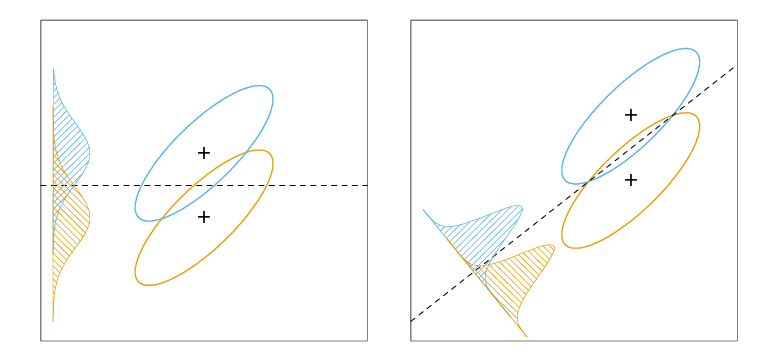
\includegraphics[width=0.8\textwidth]{image/image_1_Fisher_idea.png}
	\caption{Ý tưởng hình học của Fisher để phân tách hai lớp tốt nhất, xem tài liệu \cite{hastie2009}.}
	\label{fig:hinh1}
\end{figure}
Để lượng hóa hai ý tưởng ``cách xa nhau nhất giữa các lớp'' và ``tụ lại ở trong lớp'', Fisher đưa vào hai đại lượng cơ bản.
Gọi $\bm{\mu}$ là trung bình mẫu của toàn bộ dữ liệu. Ma trận tán xạ giữa các lớp được xác định bởi
\begin{equation}
	\Sigma_B = \sum_{k=1}^{K} n_k(\bm{\mu}_k-\bm{\mu})(\bm{\mu}_k-\bm{\mu})^T,
\end{equation}
trong đó,
\[
\bm{\mu}_k
=
\frac{1}{n_k}
\sum_{\bm{x}_i \in C_k}
\bm{x}_i,
\qquad k=1,2.
\]
là vectơ trung bình mẫu của từng lớp;
\[
\bm{\mu}
=
\frac{1}{n}
\sum_{i=1}^{n}
\bm{x}_i
\]
là vectơ trung bình mẫu của toàn bộ dữ liệu mẫu. Ma trận này phản ánh mức độ phân tách giữa các lớp thông qua vị trí tương đối của các trung bình lớp so với trung bình toàn cục.

Với mỗi lớp $C_{k}$, gọi $\bm{\mu}_k$ là vectơ trung bình mẫu của lớp đó. Ma trận tán xạ trong lớp được xác định bởi
\begin{equation}
\Sigma_W
=
\sum_{k=1}^{K}
\sum_{\bm{x}_i \in C_k}
(\bm{x}_i-\bm{\mu}_k)(\bm{x}_i-\bm{\mu}_k)^T.
\end{equation}
Ma trận này mô tả độ phân tán của các điểm quanh trung bình lớp tương ứng. Nếu các điểm trong từng lớp tập trung lại gần nhau thì $\Sigma_W$ nhỏ; ngược lại, nếu dữ liệu phân tán rộng thì $\Sigma_W$ lớn.

Trong trường hợp hai lớp, Fisher xét biến chiếu $z = \bm{\beta}^T \bm{x}$. Gọi $m_1 = \bm{\beta}^T \bm{\mu}_1$ và $m_2 = \bm{\beta}^T \bm{\mu}_2$ là trung bình của hai lớp sau chiếu. Khi đó, độ tách biệt giữa hai lớp trên phương chiếu có thể đo bằng $(m_1-m_2)^2$. Đồng thời, phương sai trong lớp sau chiếu là
\begin{equation}
\sigma_W^2 = \bm{\beta}^T \Sigma_W \bm{\beta}.
\end{equation}
Do đó, tiêu chuẩn Fisher được viết thành
\begin{equation}
J(\bm{\beta})
=
\frac{(\bm{\beta}^T(\bm{\mu}_1-\bm{\mu}_2))^2}{\bm{\beta}^T \Sigma_W \bm{\beta}}
=
\frac{\bm{\beta}^T \Sigma_B \bm{\beta}}{\bm{\beta}^T \Sigma_W \bm{\beta}}.
\end{equation}
Mục tiêu là tìm $\bm{\beta} \neq 0$ sao cho $J(\bm{\beta})$ đạt cực đại.

\subsection{Nghiệm tối ưu của Fisher trong trường hợp hai lớp}
Gọi $\bm{\mu}_1,\bm{\mu}_2$ lần lượt là vectơ trung bình của hai lớp. Khi đó, ma trận tán xạ giữa hai lớp được xác định bởi
\[
\Sigma_B
=
(\bm{\mu}_1-\bm{\mu}_2)(\bm{\mu}_1-\bm{\mu}_2)^T.
\]
Ma trận tán xạ trong lớp (ma trận phương sai mẫu gộp - pooled variance matrix) được xác định bởi
\[
\Sigma_W
=
\frac{(n_1-1)\Sigma_1+(n_2-1)\Sigma_2}{n-2},
\]
trong đó $n=n_1+n_2$, còn $\Sigma_1,\Sigma_2$ lần lượt là ma trận hiệp phương sai mẫu của hai lớp
\[
\Sigma_1
=
\frac{1}{n_1-1}
\sum_{i=1}^{n_1}
(\bm{x}_{i1}-\bm{\mu}_1)(\bm{x}_{i1}-\bm{\mu}_1)^T,
\]

\[
\Sigma_2
=
\frac{1}{n_2-1}
\sum_{i=1}^{n_2}
(\bm{x}_{i2}-\bm{\mu}_2)(\bm{x}_{i2}-\bm{\mu}_2)^T.
\]
Tiêu chuẩn Fisher được viết dưới dạng
\[
J(\bm{\beta})
=
\frac{\bm{\beta}^T\Sigma_B\bm{\beta}}
{\bm{\beta}^T\Sigma_W\bm{\beta}},
\qquad
\bm{\beta}\in\mathbb{R}^d.
\]

Mục tiêu là tìm vectơ chiếu $\bm{\beta}$ sao cho $J(\bm{\beta})$  đạt giá trị lớn nhất
\[
\max_{\bm{\beta}\neq \bm{0}}
J(\bm{\beta})
=
\max_{\bm{\beta}\neq \bm{0}}
\frac{\bm{\beta}^T\Sigma_B\bm{\beta}}
{\bm{\beta}^T\Sigma_W\bm{\beta}}.
\]
Vì $\Sigma_W$ là ma trận đối xứng xác định dương nên tồn tại phân rã phổ
\[
\Sigma_W
=
D\Lambda D^T,
\]
trong đó $D$ là ma trận trực giao chứa các vectơ riêng của $\Sigma_W$, còn $\Lambda$ là ma trận đường chéo chứa các giá trị riêng dương thỏa
\[
D^TD=I,
\qquad
\Lambda
=
\operatorname{diag}(\lambda_1,\lambda_2,\ldots,\lambda_d),
\]
với
\[
\lambda_1,\lambda_2,\ldots,\lambda_d>0.
\]

Do đó, ta đặt
\[
\Sigma_W^{1/2}
=
D\Lambda^{1/2}D^T,
\]
trong đó,
\[
\Lambda^{1/2}
=
\operatorname{diag}
\left(
\sqrt{\lambda_1},
\sqrt{\lambda_2},
\ldots,
\sqrt{\lambda_d}
\right).
\]

Tương tự, ta đặt
\[
\Sigma_W^{-1/2}
=
D\Lambda^{-1/2}D^T,
\]
với,
\[
\Lambda^{-1/2}
=
\operatorname{diag}
\left(
\frac{1}{\sqrt{\lambda_1}},
\frac{1}{\sqrt{\lambda_2}},
\ldots,
\frac{1}{\sqrt{\lambda_d}}
\right).
\]

Lúc này, với
\[
\bm{y}
=
\Sigma_W^{1/2}\bm{\beta},
\]
ta suy ra,
\[
\bm{\beta}
=
\Sigma_W^{-1/2}\bm{y}.
\tag{*}
\label{*}
\]

Thay vào tiêu chuẩn Fisher, ta được
\[
J(\bm{\beta})
=
\frac{\bm{\beta}^T \Sigma_B \bm{\beta}}
{\bm{\beta}^T \Sigma_W \bm{\beta}}
=
\frac{\bm{y}^T S \bm{y}}{\bm{y}^T \bm{y}}.
\]

Thực vậy, xét mẫu số trước
\[
\bm{\beta}^T\Sigma_W\bm{\beta}
=
\left(\Sigma_W^{-1/2}\bm{y}\right)^T
\Sigma_W
\left(\Sigma_W^{-1/2}\bm{y}\right).
\]
Vì $\Sigma_W^{-1/2}$ đối xứng nên
\[
\bm{\beta}^T\Sigma_W\bm{\beta}
=
\bm{y}^T
\Sigma_W^{-1/2}
\Sigma_W
\Sigma_W^{-1/2}
\bm{y}.
\]
Mà
\[
\begin{aligned}
	\Sigma_W^{-1/2}
	\Sigma_W
	\Sigma_W^{-1/2}
	&=
	D\Lambda^{-1/2}D^T
	D\Lambda D^T
	D\Lambda^{-1/2}D^T \\[0.2cm]
	&=
	D\Lambda^{-1/2}
	(D^TD)
	\Lambda
	(D^TD)
	\Lambda^{-1/2}D^T \\[0.2cm]
	&=
	D\Lambda^{-1/2}
	\Lambda
	\Lambda^{-1/2}D^T \\[0.2cm]
	&=
	DD^T \\[0.2cm]
	&=
	I.
\end{aligned}
\]
nên,
\[
\bm{\beta}^T\Sigma_W\bm{\beta}
=
\bm{y}^T\bm{y}.
\]

Tương tự, tử số trở thành
\[
\bm{\beta}^T\Sigma_B\bm{\beta}
=
\left(\Sigma_W^{-1/2}\bm{y}\right)^T
\Sigma_B
\left(\Sigma_W^{-1/2}\bm{y}\right).
\]
Do đó,
\[
\bm{\beta}^T\Sigma_B\bm{\beta}
=
\bm{y}^T
\left(\Sigma_W^{-1/2}\right)^T
\Sigma_B
\Sigma_W^{-1/2}
\bm{y}.
\]

Vì $\Sigma_W^{-1/2}$ đối xứng nên
\[
\left(\Sigma_W^{-1/2}\right)^T
=
\Sigma_W^{-1/2}.
\]
Đặt,
\[
S
=
\left(\Sigma_W^{-1/2}\right)^T
\Sigma_B
\Sigma_W^{-1/2}
=
\Sigma_W^{-1/2}
\Sigma_B
\Sigma_W^{-1/2}.
\]

Khi đó, tiêu chuẩn Fisher trở thành
\[
J(\bm{\beta})
=
\frac{\bm{y}^T S \bm{y}}{\bm{y}^T\bm{y}}.
\]
Vì $\Sigma_B$ đối xứng và $\Sigma_W^{-1/2}$ đối xứng nên $S$ cũng là ma trận đối xứng
\[
S^T=S.
\]
Do đó, bài toán tối ưu Fisher được đưa về bài toán
\[
\max_{\bm{y}\neq \bm{0}}
\frac{\bm{y}^T S \bm{y}}{\bm{y}^T\bm{y}}.
\]

Đây chính là bài toán thương Rayleigh.

Đặt,
\[
\bm{x}
=
\frac{\bm{y}}{\|\bm{y}\|},
\qquad
\|\bm{x}\|=1.
\]

Khi đó,
\[
\frac{\bm{y}^T S \bm{y}}{\bm{y}^T\bm{y}}
=
\bm{x}^T S \bm{x}.
\]

Vì $S$ là ma trận đối xứng xác định không âm nên tồn tại phân rã phổ
\[
S
=
U\Gamma U^T,
\]
trong đó,
\[
U^TU=I,
\]
và,
\[
\Gamma
=
\operatorname{diag}(\gamma_1,\gamma_2,\ldots,\gamma_d),
\quad \text{với} \quad
\gamma_1\geq \gamma_2\geq \cdots \geq \gamma_d \geq 0.
\]

Đặt,
\begin{equation}
	\bm{z}
	=
	U^T\bm{x}.
	\tag{**}
	\label{**}
\end{equation}

Ta có,
\[
\|\bm{z}\|^2
=
\bm{z}^T\bm{z}
=
\bm{x}^TUU^T\bm{x}
=
\bm{x}^T\bm{x}
=
1.
\]

Mặt khác,
\[
\bm{x}^T S \bm{x}
=
\bm{x}^T U\Gamma U^T\bm{x}
=
\bm{z}^T\Gamma \bm{z}.
\]

Suy ra,
\[
\bm{x}^T S \bm{x}
=
\gamma_1z_1^2
+
\gamma_2z_2^2
+
\cdots
+
\gamma_dz_d^2.
\]

Do,
\[
\gamma_1\geq \gamma_2\geq \cdots \geq \gamma_d,
\]
nên
\[
\bm{x}^T S \bm{x}
\leq
\gamma_1(z_1^2+z_2^2+\cdots+z_d^2).
\]

Mặt khác,
\[
z_1^2+z_2^2+\cdots+z_d^2
=
\|\bm{z}\|^2
=
1.
\]
nên
\[
\bm{x}^T S \bm{x}
\leq
\gamma_1.
\]

Dấu ``='' xảy ra khi và chỉ khi $\bm{z}_{\text{opt}}=(1,0,\ldots,0)^T$. Kết hợp với~\eqref{**}, ta có 
\[
\bm{x}_{\text{opt}}
=
U\bm{z}_{\text{opt}},
\]
là vectơ riêng ứng với giá trị riêng lớn nhất của $S$.

Hơn nữa, vì
\[
\bm{x}
=
\frac{\bm{y}}{\|\bm{y}\|},
\]
nên
\[
\bm{y}_{\text{opt}}
\propto
\bm{x}_{\text{opt}}.
\]

Kết hợp với~\eqref{*}, ta suy ra
\begin{equation}
	\bm{\beta}_{\text{opt}}
	\propto
	\Sigma_W^{-1/2}\bm{x}_{\text{opt}}.
	\tag{***}
	\label{***}
\end{equation}

Do $\bm{x}_{\text{opt}}$ là vectơ riêng ứng với giá trị riêng lớn nhất của $S$ nên
\[
S\bm{x}_{\text{opt}}
=
\gamma_1\bm{x}_{\text{opt}}
\quad \Longleftrightarrow \quad
\left(\Sigma_W^{-1/2}\right)^T
\Sigma_B
\left(\Sigma_W^{-1/2}\right)
\bm{x}_{\text{opt}}
=
\gamma_1\bm{x}_{\text{opt}}.
\]

Đặt, $
\bm{u}_{\text{opt}}
=
\Sigma_W^{-1/2}\bm{x}_{\text{opt}}
$, suy ra $\bm{\beta}_{\text{opt}}
\propto
\bm{u}_{\text{opt}}$ và $\bm{x}_{\text{opt}}
=
\Sigma_W^{1/2}\bm{u}_{\text{opt}}$
\[
\begin{aligned}
	\Sigma_W^{-1/2}\Sigma_B\Sigma_W^{-1/2}
	\bm{x}_{\text{opt}}
	&=
	\gamma_1\bm{x}_{\text{opt}} \\[0.2cm]
	\Sigma_W^{-1/2}\Sigma_B\Sigma_W^{-1/2}
	\Sigma_W^{1/2}\bm{u}_{\text{opt}}
	&=
	\gamma_1\Sigma_W^{1/2}\bm{u}_{\text{opt}} \\[0.2cm]
	\Sigma_W^{-1/2}\Sigma_B\bm{u}_{\text{opt}}
	&=
	\gamma_1\Sigma_W^{1/2}\bm{u}_{\text{opt}} \\[0.2cm]
	\Rightarrow \quad
	\Sigma_W^{-1}\Sigma_B\bm{u}_{\text{opt}}
	&=
	\gamma_1\bm{u}_{\text{opt}}.
\end{aligned}
\]

Lưu ý, do
\[
\Sigma_B
=
(\bm{\mu}_1-\bm{\mu}_2)(\bm{\mu}_1-\bm{\mu}_2)^T.
\]
nên
\[
\Sigma_W^{-1}
\Sigma_B
\bm{u}_{\text{opt}}
=
\Sigma_W^{-1}
(\bm{\mu}_1-\bm{\mu}_2)(\bm{\mu}_1-\bm{\mu}_2)^T
\bm{u}_{\text{opt}}.
\]

Đặt, $\bm{v}
=
\Sigma_W^{-1}(\bm{\mu}_1-\bm{\mu}_2)
\in \mathbb{R}^d,
\quad
\bm{w}
=
\bm{\mu}_1-\bm{\mu}_2$, khi đó
\[
\bm{v}\,
\underbrace{\bm{w}^T\bm{u}_{\text{opt}}}_{\in \mathbb{R}}
=
\underbrace{\bm{w}^T\bm{u}_{\text{opt}}}_{\in \mathbb{R}}\,
\bm{v}
=
\gamma_1
\bm{u}_{\text{opt}}.
\]

Suy ra $\bm{u}_{\text{opt}}
\propto
\Sigma_W^{-1}(\bm{\mu}_1-\bm{\mu}_2)$, hay
\[
\bm{\beta}_{\text{opt}}
\propto
\Sigma_W^{-1}(\bm{\mu}_1-\bm{\mu}_2).
\]

Một cách tiếp cận khác có thể sử dụng để tìm nghiệm tối ưu trên là sử dụng bất đẳng thức Cauchy--Schwarz cho tích vô hướng trong $\mathbb{R}^d$. Tuy nhiên, nội dung này sẽ không được trình bày trong phạm vi của đồ án.

Do tiêu chuẩn Fisher không thay đổi khi nhân $\bm{\beta}$ với một hằng số khác $0$, nên ta thường chọn
\[
\boxed{
	\bm{\beta}_{\text{opt}}
	=
	\Sigma_W^{-1}(\bm{\mu}_1-\bm{\mu}_2)
}
\]

Như vậy, trong trường hợp hai lớp, nghiệm tối ưu của Fisher là vectơ chiếu theo hướng nghịch đảo ma trận tán xạ trong lớp nhân với hiệu vectơ trung bình của hai lớp.

\hspace*{0.5cm}Sau khi đã xác định được phương chiếu tối ưu $\bm{\beta}_{\text{opt}}$, việc phân lớp một đối tượng có giá trị của vectơ các biến quan trắc $\bm{x}$ được thực hiện theo thủ tục sau

Với $\bm{X}=\bm{x} \in \mathbb{R}^d$, đặt $y=\bm{\beta}_{\text{opt}}^T\bm{x}$.
\[
\widehat{G}(\bm{x})
=
\arg\min_{k=1,2}
\left|y-\bar{y}_k\right|,
\]
với $\bar{y}_k=\bm{\beta}_{\text{opt}}^T\bm{\mu}_k,\ k=1,2$.

Như vậy, biên tách biệt tuyến tính của mô hình được cho bởi phương trình
\[
\left|y_{\text{bnd}}-\bar{y}_1\right|
=
\left|y_{\text{bnd}}-\bar{y}_2\right|
\]
hay
\begin{equation}
	2y_{\text{bnd}}-\left(y_1+y_2\right)=0.
	\label{eq:y-bnd}
\end{equation}

Thay $y_{\text{bnd}}=\bm{\beta}_{\text{opt}}^T\bm{x}_{\text{bnd}}$, $y_k=\bm{\beta}_{\text{opt}}^T\bm{\mu}_k \ (k=1,2)$ vào \eqref{eq:y-bnd}, với $\bm{\beta}_{\text{opt}}
=
\Sigma_W^{-1}(\bm{\mu}_1-\bm{\mu}_2)$ ta có
\[
\left[\Sigma_W^{-1}(\bm{\mu}_1-\bm{\mu}_2)\right]^T
\bm{x}_{\text{bnd}}
-
\frac{1}{2}
\left[
\bm{\mu}_1^T\Sigma_W^{-1}(\bm{\mu}_1-\bm{\mu}_2)
+
\bm{\mu}_2^T\Sigma_W^{-1}(\bm{\mu}_1-\bm{\mu}_2)
\right]
=
0
\]
\begin{equation}
	\quad \Longleftrightarrow \quad
	\left[\Sigma_W^{-1}(\bm{\mu}_1-\bm{\mu}_2)\right]^T
	\bm{x}_{\text{bnd}}
	-
	\frac{1}{2}
	\left(
	\bm{\mu}_1^T\Sigma_W^{-1}\bm{\mu}_1
	-
	\bm{\mu}_2^T\Sigma_W^{-1}\bm{\mu}_2
	\right)
	=
	0.
	\label{eq:class}
\end{equation}


























%================1.5
\section{Lý thuyết quyết định Bayes trong bài toán phân
loại}

\subsection{Xác suất hậu nghiệm và quy tắc Bayes}

Trong lý thuyết quyết định thống kê, một quy tắc phân loại được xem là tối ưu nếu nó làm cực tiểu hóa rủi ro kỳ vọng. Đối với trường hợp hàm tổn thất 0 -- 1 như đang xét trong đồ án này, bài toán tối ưu tương đương với việc cực tiểu hóa xác suất phân loại lỗi. Khi đó, quy tắc Bayes nói lên rằng: với một quan trắc $\bm{x}$, ta nên gán $\bm{x}$ vào lớp có xác suất hậu nghiệm lớn nhất. Nếu ký hiệu $\widehat{G}$ là hàm phân lớp, thì quy tắc Bayes được xác định như sau
\begin{equation}
\widehat{G}=\arg\max_k P(G=k\mid \bm{X}=\bm{x}).
\end{equation}
Theo công thức Bayes,
\begin{equation}
P(G=k\mid \bm{X}=\bm{x})=\frac{\pi_k f_k(\bm{x})}{\sum_{\ell=1}^{K}\pi_\ell f_\ell(\bm{x})},
\end{equation}
trong đó 
$f_k(\bm{x})=p(\bm{x}\,|\,G=k)$ là mật độ có điều kiện của $\bm{X}$ trong lớp $k$, còn $\pi_k=P(G=k)$ là xác suất tiên nghiệm của lớp đó. Vì mẫu số là như nhau cho mọi lớp khi so sánh, quy tắc Bayes tối ưu có thể viết gọn thành
\begin{equation}
\widehat{G}=\arg\max_k \{\pi_kf_k(\bm{x})\}.
\end{equation}

Điều này cho thấy, nếu biết đầy đủ các mật độ điều kiện và các xác suất tiên nghiệm, thì bài toán phân loại về nguyên tắc đã được giải quyết.

\subsection{LDA trong cách tiếp cận của lý thuyết quyết định Bayes}

Để áp dụng quy tắc Bayes trên một bộ phân loại cụ thể, cần giả thiết dạng của các mật độ lớp. Một giả thiết phổ biến trong phân tích thống kê nhiều chiều là mỗi lớp tuân theo phân phối chuẩn nhiều chiều. Cụ thể, với lớp $C_k$, ta giả sử
\begin{equation}
\left(\bm{X}\mid G=k\right)\sim N_d(\bm{\mu}_k,\Sigma_k),
\end{equation}

trong đó $\bm{\mu}_k$ là vectơ trung bình và $\Sigma_k$ là ma trận hiệp phương sai của lớp $k$. Khi đó, mật độ lớp có dạng

\begin{equation}
f_k(\bm{x})=\frac{1}{(2\pi)^{d/2}|\Sigma_k|^{1/2}}
\exp\left\{-\frac12(\bm{x}-\bm{\mu}_k)^T\Sigma_k^{-1}(\bm{x}-\bm{\mu}_k)\right\}.
\end{equation}

Thay biểu thức này vào quy tắc Bayes và lấy logarit cơ số \(e\), tức là logarit tự nhiên đồng thời bỏ qua các hằng số chung không phụ thuộc vào $k$. Khi đó, ta thu được hàm phân biệt
\begin{equation}
\delta_k(\bm{x})= -\frac12\ln |\Sigma_k|
-\frac12(\bm{x}-\bm{\mu}_k)^T\Sigma_k^{-1}(\bm{x}-\bm{\mu}_k)
+\ln \pi_k,
\end{equation}
Quy tắc phân loại Bayes trở thành
\begin{equation}
\widehat{G}(\bm{x})=\arg\max_k \delta_k(\bm{x}).
\end{equation}

\hspace*{0.5cm}LDA xuất hiện như một trường hợp riêng có ý nghĩa đặc biệt của mô hình Gaussian ở trên, khi giả sử tất cả các lớp có chung một ma trận hiệp phương sai, tức là
\[
\Sigma_1=\Sigma_2=\cdots=\Sigma_K=\Sigma.
\]
Trong trường hợp này, các hàm phân biệt được rút gọn thành
\begin{equation}
	\delta_k(\bm{x})=\bm{x}^T\Sigma^{-1}\bm{\mu}_k-\frac12\bm{\mu}_k^T\Sigma^{-1}\bm{\mu}_k+\ln \pi_k.
\end{equation}

Công thức này cho thấy $\delta_k(\bm{x})$ là một hàm tuyến tính theo $\bm{x}$. Do đó, biên quyết định giữa hai lớp bất kỳ $k$ và $\ell$, xác định bởi điều kiện $\delta_k(\bm{x})=\delta_\ell(\bm{x})$, có dạng
\begin{equation}
	\bm{x}^T\Sigma^{-1}(\bm{\mu}_k-\bm{\mu}_\ell)
	-\frac12\bigl(\bm{\mu}_k^T\Sigma^{-1}\bm{\mu}_k-\bm{\mu}_\ell^T\Sigma^{-1}\bm{\mu}_\ell\bigr)
	+\ln\frac{\pi_k}{\pi_\ell}=0.
\end{equation}

Đây là phương trình của một siêu phẳng trong không gian $\mathbb{R}^d$. Như vậy, dưới giả thiết phân bố trên các lớp là phân phối chuẩn nhiều chiều với cùng ma trận hiệp phương sai, quy tắc Bayes cho biên phân loại giữa 2 lớp bất kỳ là tuyến tính.

Trong trường hợp hai lớp (bài toán lưỡng phân), nếu đặt
\[
\bm{a}
=
\Sigma^{-1}(\bm{\mu}_1-\bm{\mu}_2)
\]
và
\[
b
=
-\frac12
\bigl(
\bm{\mu}_1^T\Sigma^{-1}\bm{\mu}_1
-
\bm{\mu}_2^T\Sigma^{-1}\bm{\mu}_2
\bigr)
+
\ln\frac{\pi_1}{\pi_2}.
\]
thì biên quyết định có dạng
\begin{equation}
	\bm{a}^T\bm{x}_\text{bnd}+b=0.
	\label{eq:ni}
\end{equation}

Trong thực hành, các tham số quần thể $\pi_k,\mu_k,\Sigma$ không biết trước và phải được ước lượng từ dữ liệu huấn luyện. Gọi $N$ là tổng số mẫu, $N_k$ là số mẫu thuộc lớp $k$. Các ước lượng mẫu cho các tham số quần thể được xác định như sau
\begin{equation}
	\hat{\pi}_k=\frac{N_k}{N},
	\qquad
	\hat{\bm{\mu}}_k
	=
	\frac{1}{N_k}
	\sum_{g_i=k}
	\bm{x}_i,
	\qquad (k=1,2,\ldots,K),
\end{equation}
và ma trận hiệp phương sai mẫu gộp
\begin{equation}
	\hat{\Sigma}
	=
	\frac{1}{N-K}
	\sum_{k=1}^{K}
	\sum_{g_i=k}
	(\bm{x}_i-\hat{\bm{\mu}}_k)
	(\bm{x}_i-\hat{\bm{\mu}}_k)^T.
\end{equation}

Từ đó, các hàm phân biệt ước lượng có dạng
\begin{equation}
	\hat{\delta}_k(\bm{x})
=
\bm{x}^T\hat{\Sigma}^{-1}\hat{\bm{\mu}}_k
-\frac12
\hat{\bm{\mu}}_k^T\hat{\Sigma}^{-1}\hat{\bm{\mu}}_k
+\ln\hat{\pi}_k,
\end{equation}
và quy tắc phân loại là
\begin{equation}
	\hat{G}(\bm{x})
=
\arg\max_k \hat{\delta}_k(\bm{x}).
\end{equation}

Trong bài toán hai lớp, điều này tương đương với việc kiểm tra dấu của hiệu $\hat{\delta}_1(\bm{x})-\hat{\delta}_2(\bm{x})$.

\hspace*{0.5cm}Đến đây có thể thấy rằng hai cách tiếp cận tưởng như khác nhau thực ra dẫn đến cùng một cấu trúc toán học. Theo luật quyết định Bayes, dưới giả thiết phân bố chuẩn có cùng hiệp phương sai, và $\pi_1=\pi_2$, khi đó biên tách biệt trong phương trình~\eqref{eq:ni} sẽ cho bởi phương trình
\begin{equation}
\boxed{
	\left[
	\hat{\Sigma}^{-1}
	(\hat{\bm{\mu}}_1-\hat{\bm{\mu}}_2)
	\right]^T
	\bm{x}_{\text{bnd}}
	-
	\frac{1}{2}
	\left(
	\hat{\bm{\mu}}_1^T
	\hat{\Sigma}^{-1}
	\hat{\bm{\mu}}_1
	-
	\hat{\bm{\mu}}_2^T
	\hat{\Sigma}^{-1}
	\hat{\bm{\mu}}_2
	\right)
	=
	0
}
\label{eq:class1}
\end{equation}

Đây chính là biên tách biệt tuyến tính theo cách tiếp cận của Fisher được cho trong phương trình~\eqref{eq:class} 

%================1.6
\section{Xác định độ chính xác phân loại mẫu thống kê}

Trong phạm vi đồ án này, ta chỉ xét trường hợp hàm tổn thất $0-1$. 
Điều này có nghĩa là nếu một quan sát được phân loại đúng thì chi phí phân loại bằng $0$, 
còn nếu quan sát đó bị phân loại sai thì chi phí phân loại bằng $1$, bất kể sai từ lớp $C_1$ sang $C_2$ hay từ lớp $C_2$ sang $C_1$. Khi đó, với một quan sát cỡ $n$, hiệu quả của một phương pháp phân loại được thể hiện qua ma trận nhập nhằng, hay ma trận lỗi (confusion matrix) được cho trong bảng sau 



\begin{table}[H]
	\centering
	\begin{tabular}{|c|cc|c|}
		\hline
		\multirow{2}{*}{Các lớp dự báo} & \multicolumn{2}{c|}{Các lớp đúng} & \multirow{2}{*}{Tổng cộng} \\ \cline{2-3}
		& $C_1$ & $C_2$ & \\ \hline
		$\hat{C}_1$ & $n_{11}$ & $n_{12}$ & $n_{1\bullet}$ \\
		$\hat{C}_2$ & $n_{21}$ & $n_{22}$ & $n_{2\bullet}$ \\ \hline
		Tổng cộng & $n_{\bullet 1}$ & $n_{\bullet 2}$  & $n$ \\ \hline
	\end{tabular}
	\caption{Ma trận lỗi theo tần số.}
	\label{tab:MaTranLoiTanSo}
\end{table}
Ở đây,
\begin{itemize}
	\item $n$: cỡ mẫu;
	\item $n_{ij}$: số quan sát được phân loại vào lớp $\hat{C}_i$ bởi phương pháp phân loại và thuộc lớp $C_j$ trong tập dữ liệu mẫu $(i,j=1,2)$;
	\item $n_{i\bullet}$: số quan sát được phân loại vào lớp $\hat{C}_i$ trong tập dữ liệu mẫu $(i=1,2)$;
	\item $n_{\bullet j}$: số quan sát thuộc lớp $C_j$ trong tập dữ liệu mẫu $(j=1,2)$.
\end{itemize}
Từ bảng trên, ta quan tâm đến các đại lượng đặc trưng cho độ chính xác như sau
\begin{itemize}
	\item Độ chính xác tổng thể của sự phân lớp (the overall accuracy) giữa dữ liệu được phân lớp từ phương pháp phân loại và dữ liệu tham chiếu, tức là tỷ lệ (xác suất) phân loại đúng của ánh xạ phân loại: 
	\begin{equation}
		\text{Overall Accuracy}=\frac{n_{11}+n_{22}}{n}.
		\label{eq:OverallAccuracy}
	\end{equation}
	\item Độ chính xác của thủ tục phân loại (the Producer's accuracy | Recall) là tỷ lệ (xác suất) để thủ tục phân loại gán nhãn cho một quan trắc là $\hat{C}_j$, biết rằng lớp đúng của nó là $C_j$. Điều này được thể hiện qua số đo đặc trưng 
	\begin{equation}
		P(\hat{C}_j | C_j) = \frac{n_{jj}}{n_{\bullet j}},\quad j=1,2.
		\label{eq:ProducerAccuracy}
	\end{equation}
	Trong mô hình Bayes đại lượng này chính là độ nhạy (sensitivity) và độ chuyên (specificity) của phương pháp.
	\item Độ chính xác tiên đoán, hay tỷ lệ tiên đoán đúng (precision) nghĩa là tỷ lệ lớp đúng là $C_j$ biết rằng thủ tục phân loại gán nhãn là $\hat{C}_j$. Đại lượng này được thể hiện qua số đo đặc trưng
	\begin{equation}
		P(C_j | \hat{C}_j)=\frac{n_{jj}}{n_{j\bullet}},\quad j=1,2.
		\label{eq:Precision}
	\end{equation}
	Trong mô hình Bayes, đại lượng này chính là tỷ lệ tiên đoán dương (Positive predictive Rate) và tỷ lệ tiên đoán âm (Negative Predictive Rate).
\end{itemize}

Từ ma trận xác suất lỗi, tỷ lệ  (xác suất) phân loại lỗi (Total probability of misclassification - TPM) của ánh xạ phân loại được cho bởi 
\begin{equation*}
	\text{TPM} = \frac{n_{12}+n_{21}}{n}.
\end{equation*} Lưu ý, từ công thức \ref{eq:OverallAccuracy} cho độ chính xác tổng thể của sự phân lớp ta có 
\begin{equation*}
	\text{Overall Accuracy} + \text{TPM} = 1.
\end{equation*} Sau cùng, từ Bảng \ref{tab:MaTranLoiTanSo}, ta thiết lập bảng liên quan đến các tỷ lệ (xác suất) được gọi là ma trận lỗi theo tỷ lệ, được cho ở Bảng \ref{tab:MaTranLoiTyLe}


\begin{table}[H]
	\centering
	\begin{tabular}{|c|cc|c|}
		\hline
		\multirow{2}{*}{Các lớp dự báo} & \multicolumn{2}{c|}{Các lớp đúng} & \multirow{2}{*}{Tổng cộng} \\ \cline{2-3}
		& $C_1$ & $C_2$ & \\ \hline
		$\hat{C}_1$ & $p_{11}$ & $p_{12}$ & $p_{1\bullet}$ \\
		$\hat{C}_2$ & $p_{21}$ & $p_{22}$ & $p_{2\bullet}$ \\ \hline
		Tổng cộng & $p_{\bullet 1}$ & $p_{\bullet 2}$  & $1,0$ \\ \hline
	\end{tabular}
	\caption{Ma trận lỗi theo tỷ lệ.}
	\label{tab:MaTranLoiTyLe}
\end{table}
Trong đó, 
\begin{itemize}
	\item $p_{ij}=\frac{n_{ij}}{n}$: tỷ lệ quan sát được phân loại vào lớp $\hat{C}_i$ bởi phương pháp phân loại và thuộc lớp $C_j$ trong tập dữ liệu mẫu;
	\item $p_{i\bullet}$: tỷ lệ các quan sát được phân loại vào lớp $\hat{C}_i$ trong tập dữ liệu mẫu;
	\item $p_{\bullet j}$: tỷ lệ các quan sát thuộc lớp $C_j$ trong tập dữ liệu mẫu.
\end{itemize}
với, $i,j=1,2$.
% !TeX root = ../thesis.tex
%================1.7

\section{Minh họa phân loại một chiều trên bộ dữ liệu hoa diên vỹ (Iris Dataset)}

Để minh họa cụ thể quy tắc phân loại tuyến tính trong trường hợp một chiều, ta xét bộ dữ liệu Iris của Fisher. Bộ dữ liệu này gồm ba loài hoa Iris là \textit{setosa}, \textit{versicolor} và \textit{virginica}, với bốn thuộc tính đo lường hình thái học: chiều dài đài hoa \textit{Sepal.Length}, chiều rộng đài hoa \textit{Sepal.Width}, chiều dài cánh hoa \textit{Petal.Length} và chiều rộng cánh hoa \textit{Petal.Width}. Các thuộc tính này đều được đo bằng đơn vị centimet, ký hiệu là \(\text{cm}\). Bộ dữ liệu Iris gồm tổng cộng \(150\) quan sát, trong đó mỗi loài hoa có \(50\) quan sát. Cụ thể,
\[
n_{\textit{setosa}}=n_{\textit{versicolor}}=n_{\textit{virginica}}=50.
\]
Một phần dữ liệu Iris được minh họa thông qua 6 quan sát đầu tiên như trong bảng sau
\begin{table}[H]
	\centering
	\small
	\begin{tabular}{|c|ccccc|}
		\hline
		STT & Sepal.Length & Sepal.Width & Petal.Length & Petal.Width & Species \\ \hline
		1 & 5{,}1 & 3{,}5 & 1{,}4 & 0{,}2 & setosa \\
		2 & 4{,}9 & 3{,}0 & 1{,}4 & 0{,}2 & setosa \\
		3 & 4{,}7 & 3{,}2 & 1{,}3 & 0{,}2 & setosa \\
		4 & 4{,}6 & 3{,}1 & 1{,}5 & 0{,}2 & setosa \\
		5 & 5{,}0 & 3{,}6 & 1{,}4 & 0{,}2 & setosa \\
		6 & 5{,}4 & 3{,}9 & 1{,}7 & 0{,}4 & setosa \\ \hline
	\end{tabular}
	\caption{6 quan sát đầu tiên của bộ dữ liệu Iris.}
	\label{tab:SauDongDauIris}
\end{table}

Hình \ref{fig:iris_petal_length_width} biểu diễn đám mây điểm của ba lớp hoa Iris theo hai thuộc tính \textit{Petal.Length} và \textit{Petal.Width}. Qua hình này, ta thấy lớp \textit{setosa} được tách biệt khá rõ so với hai lớp còn lại, trong khi hai lớp \textit{versicolor} và \textit{virginica} có vùng gần nhau hơn.

\begin{figure}[H]
	\centering
	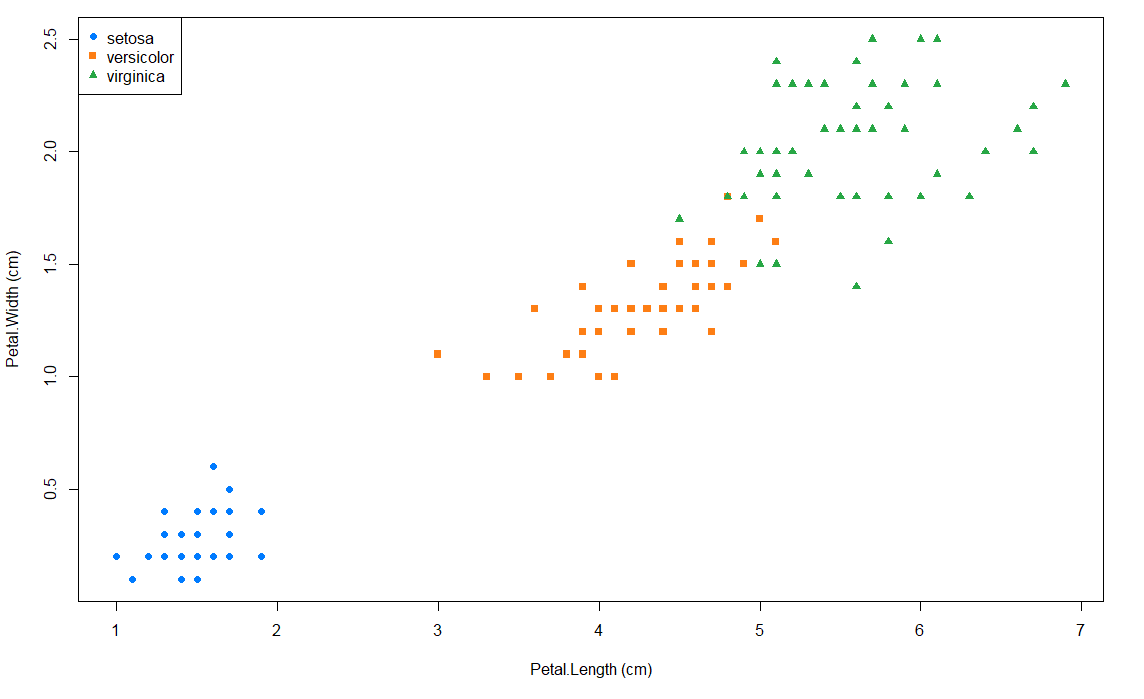
\includegraphics[width=0.85\textwidth]{image/iris_test.png}
	\caption{Đám mây điểm của ba lớp trong bộ dữ liệu Iris theo hai thuộc tính \textit{Petal.Length} và \textit{Petal.Width}.}
	\label{fig:iris_petal_length_width}
\end{figure}
Trong ví dụ này, ta chỉ xét hai lớp hoa
\[
C_1=\textit{versicolor}, \qquad C_2=\textit{virginica},
\]
và chỉ sử dụng một thuộc tính duy nhất là chiều dài cánh hoa, ký hiệu bởi
\[
x=\text{Petal.Length}.
\]
Như vậy, bài toán phân loại nhiều chiều ban đầu được rút gọn thành bài toán phân loại một chiều trên trục thực.

Gọi $\textbf{x}_1$ là tập các quan sát thuộc lớp \textit{versicolor} và $\textbf{x}_2$ là tập các quan sát thuộc lớp \textit{virginica}. Từ dữ liệu Iris, ta có
\[
n_1=n_2=50,
\]
do đó xác suất tiên nghiệm của hai lớp là
\[
\hat\pi_1=\hat\pi_2=\frac{1}{2}.
\]

Trung bình mẫu của thuộc tính \textit{Petal.Length} trong hai lớp lần lượt là
\[
\hat{\mu}_1 = 4{,}260\ (\text{cm}), \qquad
\hat{\mu}_2 = 5{,}552\ (\text{cm}).
\]
Phương sai mẫu của hai lớp là
\[
s_1^2 = 0{,}2208\ (\text{cm}^2), \qquad
s_2^2 = 0{,}3046\ (\text{cm}^2).
\]
Vì LDA giả thiết hai lớp có chung phương sai trong trường hợp một chiều, phương sai gộp được ước lượng bởi
\[
s_p^2=
\frac{(n_1-1)s_1^2+(n_2-1)s_2^2}{n_1+n_2-2}.
\]
Thay số vào ta được
\[
s_p^2
=
\frac{49(0{,}2208)+49(0{,}3046)}{98}
\approx 0{,}2627\;(\text{cm}^2).
\]

Trong trường hợp một chiều, hàm tách biệt LDA của lớp $k$ có dạng
\[
\hat\delta_k(x)
=
x\frac{\hat\mu_k}{s_p^2}
-
\frac{1}{2}\frac{\hat\mu_k^2}{s_p^2}
+
\ln \hat\pi_k,
\qquad k=1,2.
\]
Biên quyết định giữa hai lớp được xác định bởi điều kiện
\[
\hat{\delta}_1(x)=\hat{\delta}_2(x).
\]
Giải phương trình này theo $x$, ta thu được ngưỡng phân loại
\[
x_{\text{bnd}}
=
\frac{\hat\mu_1+\hat\mu_2}{2}
-
\frac{s_p^2}{\hat\mu_2-\hat\mu_1}
\ln\frac{\hat\pi_2}{\hat\pi_1}.
\]
Trong ví dụ này, do hai lớp có cùng số quan sát nên
\[
\hat\pi_1=\hat\pi_2,
\]
suy ra
\[
\ln\frac{\hat\pi_2}{\hat\pi_1}=0.
\]
Vì vậy, ngưỡng phân loại trở thành trung điểm giữa hai trung bình
\[
x_{\text{bnd}}
=
\frac{\hat{\mu}_1+\hat{\mu}_2}{2}
=
\frac{4{,}260+5{,}552}{2}
=
4{,}906\;(\text{cm}).
\]

Do $\hat\mu_2>\hat\mu_1$, quy tắc phân loại LDA trong trường hợp này là
\[
\hat G(x)=
\begin{cases}
	C_1, & x \leq 4{,}906\;(\text{cm}),\\
	C_2, & x > 4{,}906\;(\text{cm}).
\end{cases}
\]
Hay viết cụ thể theo tên loài hoa
\[
\hat G(x)=
\begin{cases}
	\textit{versicolor}, & \text{nếu } \text{Petal.Length}\leq 4{,}906\;(\text{cm}),\\
	\textit{virginica}, & \text{nếu } \text{Petal.Length}>4{,}906\;(\text{cm}).
\end{cases}
\]

Hình~\ref{fig:lda_iris_1d} biểu diễn hai mật độ Gaussian một chiều được ước lượng từ dữ liệu của hai lớp \textit{versicolor} và \textit{virginica}. Hai đường cong được vẽ dưới dạng $\hat\pi_k f_k(x)$, tức là mật độ nhân với xác suất tiên nghiệm của lớp tương ứng. Đường thẳng đứng nét đứt màu đen biểu diễn ngưỡng phân loại LDA tại $x_{\text{bnd}}=4{,}906\;(\text{cm})$.

\begin{figure}[H]
	\centering
	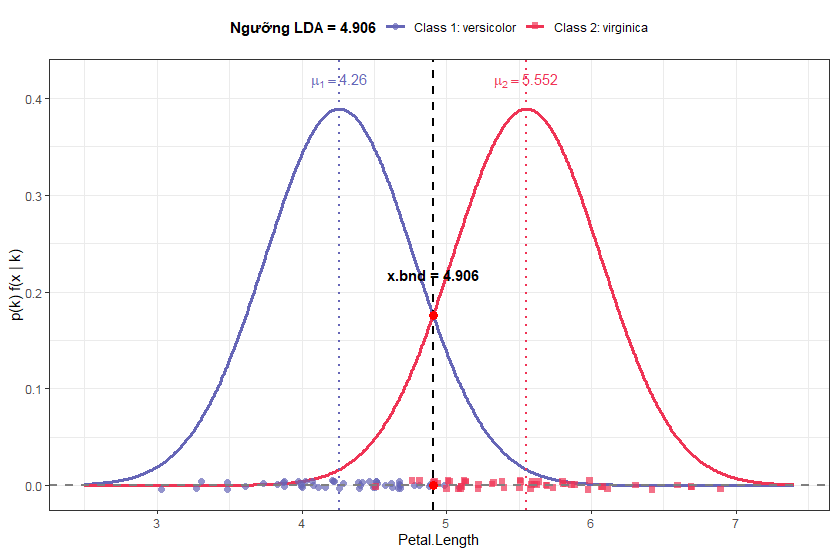
\includegraphics[width=0.85\textwidth]{image/bayes1D.png}
	\caption{Minh họa phân loại một chiều bằng LDA trên bộ dữ liệu Iris với hai lớp \textit{versicolor} và \textit{virginica} theo thuộc tính \textit{Petal.Length}.}
	\label{fig:lda_iris_1d}
\end{figure}

Từ hình minh họa có thể thấy phân phối của lớp \textit{versicolor} tập trung chủ yếu về phía bên trái, trong khi phân phối của lớp \textit{virginica} tập trung về phía bên phải. Tuy nhiên, hai phân phối vẫn có một vùng chồng lấn xung quanh ngưỡng phân loại. Đây chính là vùng mà khả năng phân loại sai có thể xảy ra.

Kết quả phân loại trên 100 quan sát thuộc hai lớp cho ma trận lỗi như sau
\[
\begin{array}{c|cc}
	& \text{versicolor} & \text{virginica} \\
	\hline
	\text{Dự đoán versicolor} & 48 & 6 \\
	\text{Dự đoán virginica} & 2 & 44
\end{array}
\]
Do đó, số quan sát bị phân loại sai là
\[
2+6=8.
\]
Tỷ lệ phân loại sai là
\[
\frac{8}{100}=0{,}08=8\%.
\]
Như vậy, trong ví dụ một chiều này, bộ phân loại LDA đạt tỷ lệ lỗi xấp xỉ $8\%$.
Ví dụ trên cho thấy khi giả thiết hai lớp có phân phối Gaussian với cùng phương sai, biên quyết định LDA trong không gian một chiều chỉ là một điểm cắt trên trục số. Các quan sát nằm về một phía của điểm cắt được gán vào lớp thứ nhất, còn các quan sát nằm về phía còn lại được gán vào lớp thứ hai. Đây là dạng đơn giản nhất của biên tuyến tính trong LDA.

\hspace*{0.5cm}Ở ví dụ trước, hai lớp \textit{versicolor} và \textit{virginica} có vùng giao nhau nên LDA vẫn có thể phát sinh lỗi phân loại. Để minh họa trường hợp biên quyết định một chiều có thể phân tách hoàn toàn dữ liệu, ta xét một cặp hoa khác trong bộ dữ liệu Iris, đó là \textit{setosa} và \textit{versicolor}, tiếp tục với thuộc tính phân loại là \textit{Petal.Length}.

Gọi
\[
C_1=\textit{setosa}, \qquad C_2=\textit{versicolor},
\]
và
\[
x=\text{Petal.Length}.
\]
Khi đó, mỗi quan sát được biểu diễn bởi một giá trị thực trên trục một chiều.

Từ bộ dữ liệu Iris, mỗi lớp có 50 quan sát, do đó
\[
n_1=n_2=50.
\]
Suy ra xác suất tiên nghiệm của hai lớp là
\[
\hat{\pi}_1=\hat{\pi}_2=\frac{1}{2}.
\]

Trung bình mẫu của thuộc tính \textit{Petal.Length} trong hai lớp lần lượt là
\[
\hat{\mu}_1=1{,}462\;(\text{cm}), 
\qquad 
\hat{\mu}_2=4{,}260\;(\text{cm}).
\]
Trong đó, $\hat{\mu}_1$ là trung bình của lớp \textit{setosa}, còn $\hat{\mu}_2$ là trung bình của lớp \textit{versicolor}. Phương sai mẫu tương ứng là
\[
s_1^2=0{,}0302\;(\text{cm}^2), 
\qquad 
s_2^2=0{,}2208\;(\text{cm}^2).
\]

Phương sai gộp được tính bởi
\[
s_p^2
=
\frac{(n_1-1)s_1^2+(n_2-1)s_2^2}{n_1+n_2-2}.
\]
Thay số vào ta được
\[
s_p^2
=
\frac{49(0{,}0302)+49(0{,}2208)}{98}
\approx
0{,}1255\;(\text{cm}^2).
\]

Trong trường hợp một chiều, hàm tách biệt LDA của lớp $k$ có dạng
\[
\hat{\delta}_k(x)
=
x\frac{\hat{\mu}_k}{s_p^2}
-
\frac{1}{2}\frac{\hat{\mu}_k^2}{s_p^2}
+
\ln\hat{\pi}_k,
\qquad k=1,2.
\]
Biên quyết định giữa hai lớp được xác định bởi điều kiện
\[
\hat{\delta}_1(x)=\hat{\delta}_2(x).
\]
Giải phương trình trên theo $x$, ta thu được ngưỡng phân loại
\[
x_{\text{bnd}}
=
\frac{\hat{\mu}_1+\hat{\mu}_2}{2}
-
\frac{s_p^2}{\hat{\mu}_2-\hat{\mu}_1}
\ln\frac{\hat{\pi}_2}{\hat{\pi}_1}.
\]

Do hai lớp có cùng số quan sát nên
\[
\hat{\pi}_1=\hat{\pi}_2.
\]
Suy ra
\[
\ln\frac{\hat{\pi}_2}{\hat{\pi}_1}=0.
\]
Vì vậy, ngưỡng phân loại trở thành
\[
x_{\text{bnd}}
=
\frac{\hat{\mu}_1+\hat{\mu}_2}{2}
=
\frac{1{,}462+4{,}260}{2}
\approx
2{,}861\;(\text{cm}).
\]

Mặt khác, trong dữ liệu thực tế, giá trị lớn nhất của \textit{Petal.Length} đối với lớp \textit{setosa} là
\[
\max(\textit{setosa})=1{,}9\;(\text{cm}),
\]
trong khi giá trị nhỏ nhất của \textit{Petal.Length} đối với lớp \textit{versicolor} là
\[
\min(\textit{versicolor})=3{,}0\;(\text{cm}).
\]
Do đó
\[
1{,}9 < 3{,}0.
\]
Điều này cho thấy hai lớp \textit{setosa} và \textit{versicolor} được tách biệt hoàn toàn theo thuộc tính \textit{Petal.Length}. Khoảng trống giữa hai lớp là từ $1{,}9$ đến $3{,}0$ cm.

Ngưỡng LDA
\[
x_{\text{bnd}}\approx 2{,}861\;(\text{cm})
\]
nằm trong khoảng trống này, nên có thể phân loại đúng toàn bộ các quan sát thuộc hai lớp.

Do $\hat{\mu}_2>\hat{\mu}_1$, quy tắc phân loại LDA trong ví dụ này là
\[
\hat{G}(x)=
\begin{cases}
	\textit{setosa}, & \text{nếu } \text{Petal.Length}\leq 2{,}861\;(\text{cm}),\\
	\textit{versicolor}, & \text{nếu } \text{Petal.Length}>2{,}861\;(\text{cm}).
\end{cases}
\]

Hình~\ref{fig:lda_iris_setosa_versicolor} minh họa hai phân phối một chiều của hai lớp \textit{setosa} và \textit{versicolor} theo thuộc tính \textit{Petal.Length}. Đường thẳng đứng nét đứt màu đen biểu diễn ngưỡng phân loại LDA. Các điểm dữ liệu thực tế của hai lớp nằm ở hai phía khác nhau của ngưỡng, cho thấy sự tách biệt hoàn toàn trong trường hợp này.

\begin{figure}[H]
	\centering
	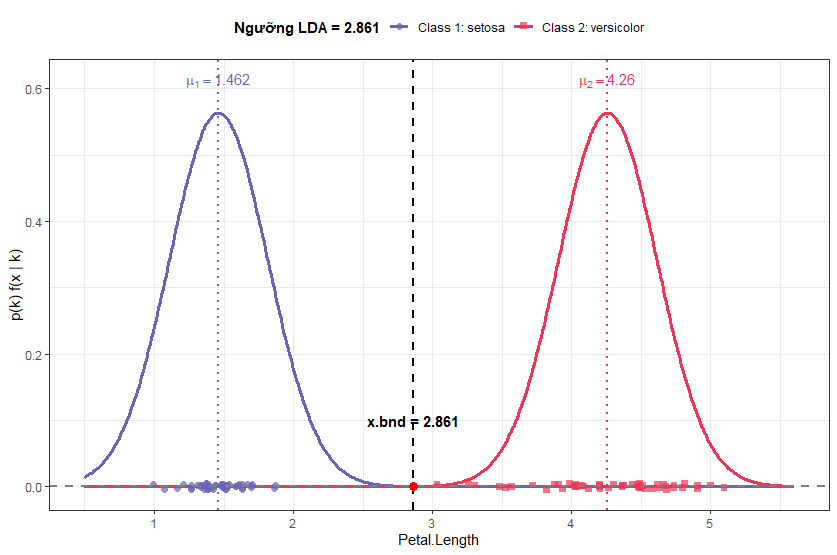
\includegraphics[width=0.85\textwidth]{image/bayes1Dgood.png}
	\caption{Minh họa phân loại một chiều bằng LDA trên bộ dữ liệu Iris với hai lớp \textit{setosa} và \textit{versicolor} theo thuộc tính \textit{Petal.Length}.}
	\label{fig:lda_iris_setosa_versicolor}
\end{figure}

Kết quả phân loại trên 100 quan sát thuộc hai lớp \textit{setosa} và \textit{versicolor} cho ma trận lỗi
\[
\begin{array}{c|cc}
	& \textit{setosa} & \textit{versicolor} \\
	\hline
	\text{Dự đoán setosa} & 50 & 0 \\
	\text{Dự đoán versicolor} & 0 & 50
\end{array}
\]
Từ ma trận trên, không có quan sát nào bị phân loại sai. Do đó, tỷ lệ lỗi phân loại là
\[
\frac{0}{100}=0.
\]

Ví dụ này cho thấy trong trường hợp một chiều, nếu hai lớp có sự tách biệt rõ ràng trên một thuộc tính, biên quyết định của LDA chỉ là một điểm cắt trên trục số và có thể phân loại hoàn toàn chính xác các quan sát trong dữ liệu. Trường hợp \textit{setosa} và \textit{versicolor} với thuộc tính \textit{Petal.Length} là một minh họa điển hình cho khả năng phân tách tuyến tính của LDA trong không gian một chiều.




\chapter {LDA cho bài toán phân loại trên dữ liệu mô phỏng}


%================2.1
% \section{Bài toán phân loại hai lớp}

Xét bài toán phân loại hai lớp $C_1$ và $C_2$. Mỗi đối tượng cần phân loại được biểu diễn bởi vectơ đặc trưng
\[
\bm{X}=\bm{x}\in\mathbb{R}^d.
\]

Trong chương này, ta sử dụng các kết quả đã chứng minh ở Chương 1 để xây dựng quy tắc phân loại Fisher và đánh giá độ chính xác phân loại trên dữ liệu mô phỏng.

\section{Thiết lập bài toán và giả thiết mô hình xác suất}

Giả sử hai lớp trên có phân phối chuẩn nhiều chiều với cùng ma trận hiệp phương sai
\[
(\bm{X}\mid C_k) \sim N_d(\bm{\mu}_k,\Sigma),
\qquad k=1,2.
\]
Trong đó $\bm{\mu}_1,\bm{\mu}_2$ là vectơ trung bình của hai lớp và $\Sigma$ là ma trận hiệp phương sai chung. Trong phạm vi đồ án, ta xét hàm tổn thất $0-1$, tức là phân loại đúng có chi phí bằng $0$ và phân loại sai có chi phí bằng $1$.

Từ kết quả đã chứng minh ở Chương 1, phương chiếu tối ưu của Fisher trong trường hợp hai lớp là
\[
\bm{\beta}_{\text{opt}}
=
\Sigma_W^{-1}(\bm{\mu}_1-\bm{\mu}_2).
\]

Với giả thiết hai lớp có chung ma trận hiệp phương sai, $\Sigma_W$ đóng vai trò tương ứng với $\Sigma$. Khi đó, ta có thể viết
\[
\bm{\beta}_{\text{opt}}
=
\Sigma^{-1}(\bm{\mu}_1-\bm{\mu}_2),
\]
và biên tách biệt tuyến tính được cho bởi phương trình
\begin{equation}
	\begin{aligned}
		&\left[{\Sigma}_W^{-1}(\bm{\mu}_1-\bm{\mu}_2)\right]^T
		\bm{x}_{\text{bnd}}
		-
		\frac{1}{2}
		\left(
		\bm{\mu}_1^T{\Sigma}_W^{-1}\bm{\mu}_1
		-
		\bm{\mu}_2^T{\Sigma}_W^{-1}\bm{\mu}_2
		\right)
		=0
	\end{aligned}
	\label{eq:immmm}
\end{equation}
Ta có \[ \bm{\mu}_1^T\Sigma_W^{-1}\bm{\mu}_1 - \bm{\mu}_2^T\Sigma_W^{-1}\bm{\mu}_2 \] \[ = \bm{\mu}_1^T\Sigma_W^{-1}\bm{\mu}_1 + \bm{\mu}_1^T\Sigma_W^{-1}\bm{\mu}_2 - \bm{\mu}_2^T\Sigma_W^{-1}\bm{\mu}_1 - \bm{\mu}_2^T\Sigma_W^{-1}\bm{\mu}_2. \] Vì \(\Sigma_W^{-1}\) là ma trận đối xứng nên \[ \bm{\mu}_1^T\Sigma_W^{-1}\bm{\mu}_2 = \bm{\mu}_2^T\Sigma_W^{-1}\bm{\mu}_1. \] Do đó, việc thêm bớt hai hạng tử chéo ở trên không làm thay đổi giá trị biểu thức. Nhóm các hạng tử lại, ta được \[ \bm{\mu}_1^T\Sigma_W^{-1}\bm{\mu}_1 + \bm{\mu}_1^T\Sigma_W^{-1}\bm{\mu}_2 - \bm{\mu}_2^T\Sigma_W^{-1}\bm{\mu}_1 - \bm{\mu}_2^T\Sigma_W^{-1}\bm{\mu}_2 \] \[ = \bm{\mu}_1^T\Sigma_W^{-1}(\bm{\mu}_1+\bm{\mu}_2) - \bm{\mu}_2^T\Sigma_W^{-1}(\bm{\mu}_1+\bm{\mu}_2) \] \[ = (\bm{\mu}_1-\bm{\mu}_2)^T \Sigma_W^{-1} (\bm{\mu}_1+\bm{\mu}_2). \] Mặt khác, do \(\Sigma_W^{-1}\) đối xứng nên \[ (\bm{\mu}_1-\bm{\mu}_2)^T\Sigma_W^{-1} = \left[ \Sigma_W^{-1}(\bm{\mu}_1-\bm{\mu}_2) \right]^T. \] Từ đó \[ \bm{\mu}_1^T\Sigma_W^{-1}\bm{\mu}_1 - \bm{\mu}_2^T\Sigma_W^{-1}\bm{\mu}_2 = \left[ \Sigma_W^{-1}(\bm{\mu}_1-\bm{\mu}_2) \right]^T (\bm{\mu}_1+\bm{\mu}_2). \]
Do đó phương trình\eqref{eq:immmm} thành,
\[
\bm{\beta}_{\text{opt}}^T\bm{x}_{\text{bnd}}
-
\frac{1}{2}
\bm{\beta}_{\text{opt}}^T
(\bm{\mu}_1+\bm{\mu}_2)
=
0.
\]

Suy ra phương trình biên tách biệt có dạng
\begin{equation}
	\bm{\beta}_{\text{opt}}^T
	\left(
	\bm{x}_{\text{bnd}}
	-
	\frac{\bm{\mu}_1+\bm{\mu}_2}{2}
	\right)
	=
	0.
	\tag{2.2}
\end{equation}


\hspace*{0.5cm}Trong thực tế, các tham số tổng thể $\mu_1,\mu_2,\Sigma$ thường chưa biết nên được thay bằng các ước lượng mẫu. Gọi $D_1,D_2$ lần lượt là tập dữ liệu huấn luyện của hai lớp, với kích thước mẫu $n_1,n_2$. Trung bình mẫu của từng lớp là
\[
\hat{\bm{\mu}}_k
=
\frac{1}{n_k}
\sum_{\bm{x}_i\in D_k}
\bm{x}_i,
\qquad k=1,2.
\]

Ma trận hiệp phương sai mẫu gộp là
\[
\hat{\Sigma}
=
S_p
=
\frac{(n_1-1)\hat{\Sigma}_1+(n_2-1)\hat{\Sigma}_2}{n_1+n_2-2}.
\]

Khi đó, phương chiếu Fisher thực nghiệm được xác định bởi
\[
\bm{b}_{\text{opt}}
=
\hat{\Sigma}^{-1}(\hat{\bm{\mu}}_1-\hat{\bm{\mu}}_2).
\]

Hàm tách biệt thực nghiệm thỏa phương trình
\begin{equation}
	\bm{b}_{\text{opt}}^T
	\left(
	\bm{x}_{\text{bnd}}
	-
	\frac{\widehat{\bm{\mu}}_1+\widehat{\bm{\mu}}_2}{2}
	\right)
	=
	0.
	\tag{2.3}
\end{equation}

\section{Thực nghiệm bài toán phân loại hai chiều trên dữ liệu mô phỏng}
\subsection{Mô phỏng trường hợp hai lớp ít chồng lấp}

Xét bài toán phân loại với dữ liệu hai chiều $(d=2)$. Dữ liệu được sinh ngẫu nhiên từ hai phân phối chuẩn hai chiều có cùng ma trận hiệp phương sai.

Thiết lập các tham số của dữ liệu mô phỏng như sau
\[
n_1=n_2=500.
\]
\[
\bm{\mu}_1=
\begin{pmatrix}
	3\\
	3
\end{pmatrix},
\qquad
\bm{\mu}_2=
\begin{pmatrix}
	4\\
	4
\end{pmatrix}.
\]
\[
\Sigma
=
\begin{pmatrix}
2 & -1{,}5\\
-1{,}5 & 2
\end{pmatrix}.
\]
Trước hết, ta xác định biên LDA lý thuyết từ các tham số đã thiết lập ban đầu. Trong trường hợp hai lớp có cùng ma trận hiệp phương sai và xác suất tiên nghiệm bằng nhau, biên quyết định lý thuyết được xác định bởi
\[
\bm{\beta}_{\text{opt}}
=
\Sigma^{-1}(\bm{\mu}_1-\bm{\mu}_2),
\]
và
\[
\bm{\beta}_{\text{opt}}^T
\left(
\bm{x}_{\text{bnd}}
-
\frac{\bm{\mu}_1+\bm{\mu}_2}{2}
\right)
=
0.
\]

Với
\[
\bm{\mu}_1=
\begin{pmatrix}
	3\\
	3
\end{pmatrix},
\qquad
\bm{\mu}_2=
\begin{pmatrix}
	4\\
	4
\end{pmatrix},
\qquad
\Sigma=
\begin{pmatrix}
	2 & -1{,}5\\
	-1{,}5 & 2
\end{pmatrix},
\]
ta có
\[
\Sigma^{-1}
=
\begin{pmatrix}
	1{,}1429 & 0{,}8571\\
	0{,}8571 & 1{,}1429
\end{pmatrix}.
\]

Do đó,
\[
\begin{aligned}
	\bm{\beta}_{\text{opt}}
	&=
	\Sigma^{-1}(\bm{\mu}_1-\bm{\mu}_2) \\[0.2cm]
	&=
	\begin{pmatrix}
		1{,}1429 & 0{,}8571\\
		0{,}8571 & 1{,}1429
	\end{pmatrix}
	\left[
	\begin{pmatrix}
		3\\
		3
	\end{pmatrix}
	-
	\begin{pmatrix}
		4\\
		4
	\end{pmatrix}
	\right] \\[0.2cm]
	&=
	\begin{pmatrix}
		1{,}1429 & 0{,}8571\\
		0{,}8571 & 1{,}1429
	\end{pmatrix}
	\begin{pmatrix}
		-1\\
		-1
	\end{pmatrix} \\[0.2cm]
	&=
	\begin{pmatrix}
		-2\\
		-2
	\end{pmatrix}.
\end{aligned}
\]

Trung điểm của hai vectơ trung bình lý thuyết là
\[
\frac{\bm{\mu}_1+\bm{\mu}_2}{2}
=
\begin{pmatrix}
	3{,}5\\
	3{,}5
\end{pmatrix}.
\]

Vì vậy, biên LDA lý thuyết thỏa mãn
\[
\begin{pmatrix}
	-2 & -2
\end{pmatrix}
\left[
\bm{x}_{\text{bnd}}
-
\begin{pmatrix}
	3{,}5\\
	3{,}5
\end{pmatrix}
\right]
=
0.
\]

Đặt
\[
\bm{x}_{\text{bnd}}
=
\begin{pmatrix}
	x_1\\
	x_2
\end{pmatrix},
\]
ta được
\[
-2(x_1-3{,}5)-2(x_2-3{,}5)=0.
\]

Khai triển, ta có
\[
-2x_1-2x_2+14=0.
\]

Do đó, phương trình biên LDA lý thuyết là
\[
-2x_1-2x_2+14=0.
\]

Tương đương,
\[
x_2=7-x_1.
\]

Biên LDA lý thuyết này được dùng để so sánh với biên LDA thực nghiệm được ước lượng từ dữ liệu mô phỏng. Trong quá trình phân loại thực nghiệm, ta sử dụng biên LDA thực nghiệm dựa trên các ước lượng mẫu \(\hat{\bm{\mu}}_1,\hat{\bm{\mu}}_2\) và \(\hat{\Sigma}\), không sử dụng trực tiếp biên lý thuyết.

Từ các tham số thiết lập mô phỏng trên, ta sinh ngẫu nhiên tập dữ liệu của hai lớp
\[
D_1=\{\bm{x}_{11},\bm{x}_{21},\ldots,\bm{x}_{n_1 1}\},
\qquad
D_2=\{\bm{x}_{12},\bm{x}_{22},\ldots,\bm{x}_{n_2 2}\}.
\]

Sau khi có dữ liệu mô phỏng, các tham số dùng trong bộ phân loại LDA không lấy trực tiếp từ thiết lập ban đầu mà được ước lượng từ mẫu. Cụ thể, xác suất tiên nghiệm của hai lớp được ước lượng bởi
\[
\hat{\pi}_1=\frac{n_1}{n_1+n_2},
\qquad
\hat{\pi}_2=\frac{n_2}{n_1+n_2}.
\]

Vectơ trung bình mẫu của hai lớp là
\[
\hat{\bm{\mu}}_1
=
\frac{1}{n_1}
\sum_{\bm{x}_i\in D_1}
\bm{x}_i,
\qquad
\hat{\bm{\mu}}_2
=
\frac{1}{n_2}
\sum_{\bm{x}_i\in D_2}
\bm{x}_i.
\]
Gọi \(\hat{\Sigma}_1,\hat{\Sigma}_2\) lần lượt là ma trận hiệp phương sai mẫu của hai lớp. Ma trận hiệp phương sai mẫu gộp được xác định bởi \[ \hat{\Sigma} = \frac{(n_1-1)\hat{\Sigma}_1+(n_2-1)\hat{\Sigma}_2}{n_1+n_2-2}. \]
Từ dữ liệu mô phỏng, ta thu được các ước lượng mẫu như sau
\[
\hat{\pi}_1=0{,}5,
\qquad
\hat{\pi}_2=0{,}5.
\]

Vectơ trung bình mẫu của hai lớp lần lượt là
\[
\hat{\bm{\mu}}_1
=
\begin{pmatrix}
	3{,}0345\\
	2{,}9611
\end{pmatrix},
\qquad
\hat{\bm{\mu}}_2
=
\begin{pmatrix}
	4{,}0687\\
	3{,}9000
\end{pmatrix}.
\]

Ma trận hiệp phương sai mẫu của lớp thứ nhất và lớp thứ hai lần lượt là
\[
\hat{\Sigma}_1
=
\begin{pmatrix}
	2{,}1348 & -1{,}6155\\
	-1{,}6155 & 2{,}1642
\end{pmatrix},
\qquad
\hat{\Sigma}_2
=
\begin{pmatrix}
	2{,}3551 & -1{,}8622\\
	-1{,}8622 & 2{,}3289
\end{pmatrix}.
\]

Do đó, ma trận hiệp phương sai mẫu gộp được ước lượng bởi
\[
\hat{\Sigma}
=
S_p
=
\begin{pmatrix}
	2{,}2449 & -1{,}7388\\
	-1{,}7388 & 2{,}2465
\end{pmatrix}.
\]
\[
\Rightarrow
\hat{\Sigma}^{-1}
=
\begin{pmatrix}
	1{,}1123 & 0{,}8609\\
	0{,}8609 & 1{,}1115
\end{pmatrix}.
\]

Khi đó, phương chiếu Fisher thực nghiệm được xác định bởi
\[
\begin{aligned}
	\bm{b}_{\text{opt}}
	&=
	\hat{\Sigma}^{-1}
	(\hat{\bm{\mu}}_1-\hat{\bm{\mu}}_2) \\[0.2cm]
	&=
	\begin{pmatrix}
		1{,}1123 & 0{,}8609\\
		0{,}8609 & 1{,}1115
	\end{pmatrix}
	\left[
	\begin{pmatrix}
		3{,}0345\\
		2{,}9611
	\end{pmatrix}
	-
	\begin{pmatrix}
		4{,}0687\\
		3{,}9000
	\end{pmatrix}
	\right] \\[0.2cm]
	&=
	\begin{pmatrix}
		1{,}1123 & 0{,}8609\\
		0{,}8609 & 1{,}1115
	\end{pmatrix}
	\begin{pmatrix}
		-1{,}0343\\
		-0{,}9389
	\end{pmatrix} \\[0.2cm]
	&=
	\begin{pmatrix}
		-1{,}9587\\
		-1{,}9340
	\end{pmatrix}.
\end{aligned}
\]

Biên phân loại LDA được xác định bởi phương trình
\[
\bm{b}_{\text{opt}}^T
\left(
\bm{x}_{\text{bnd}}
-
\frac{\hat{\bm{\mu}}_1+\hat{\bm{\mu}}_2}{2}
\right)
=
0.
\]
Trung điểm của hai vectơ trung bình mẫu là
\[
\frac{\hat{\bm{\mu}}_1+\hat{\bm{\mu}}_2}{2}
=
\begin{pmatrix}
	3{,}5516\\
	3{,}4306
\end{pmatrix}.
\]
Thay số vào phương trình trên, ta được
\[
\begin{pmatrix}
	-1{,}9587 & -1{,}9340
\end{pmatrix}
\left[
\bm{x}_{\text{bnd}}
-
\begin{pmatrix}
	3{,}5516\\
	3{,}4306
\end{pmatrix}
\right]
=
0.
\]

Đặt
\[
\bm{x}_{\text{bnd}}
=
\begin{pmatrix}
	x_1\\
	x_2
\end{pmatrix}.
\]

Khi đó,
\[
\begin{pmatrix}
	-1{,}9587 & -1{,}9340
\end{pmatrix}
\left[
\begin{pmatrix}
	x_1\\
	x_2
\end{pmatrix}
-
\begin{pmatrix}
	3{,}5516\\
	3{,}4306
\end{pmatrix}
\right]
=
0.
\]

Suy ra
\[
-1{,}9587(x_1-3{,}5516)
-
1{,}9340(x_2-3{,}4306)
=
0.
\]

Khai triển, ta được
\[
-1{,}9587x_1
-
1{,}9340x_2
+
13{,}5912
=
0.
\]
Do đó, phương trình biên phân loại LDA có dạng
\[
-1{,}9587x_1
-
1{,}9340x_2
+
13{,}5912
=
0.
\]
Tương đương,
\[
x_2
=
7{,}0276
-
1{,}0128x_1.
\]
\begin{figure}[H]
    \centering
    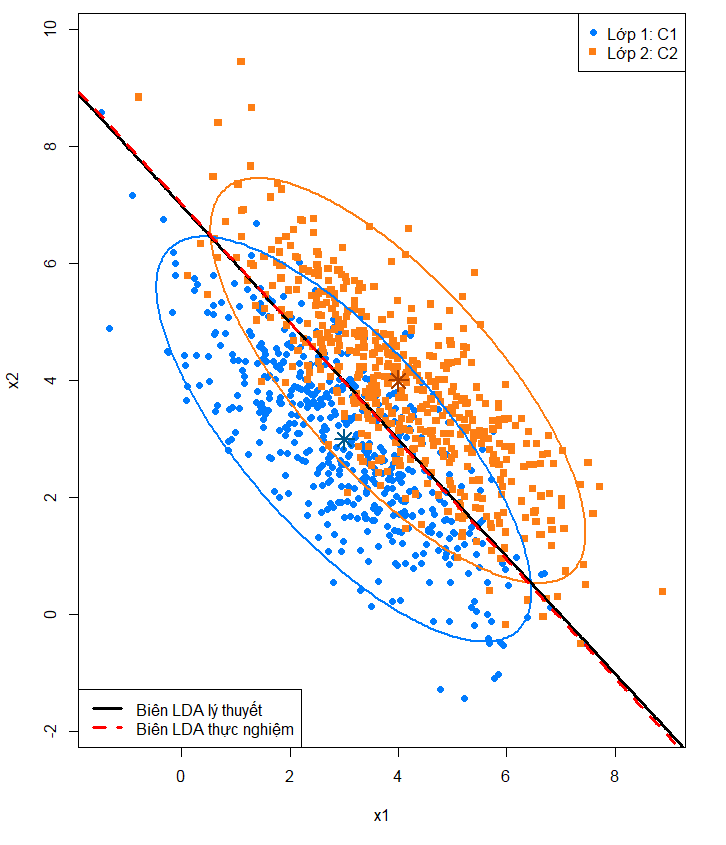
\includegraphics[width=0.8\textwidth]{image/normal_dis_2_classes_test.png}
    \caption{Phân bố mẫu của hai lớp chuẩn hai chiều và biên phân loại LDA.}
    \label{fig:2d_normal_class}
\end{figure}

\clearpage

Để đánh giá kết quả phân loại, ta sử dụng ma trận lỗi.
\begin{figure}[H]
    \centering
    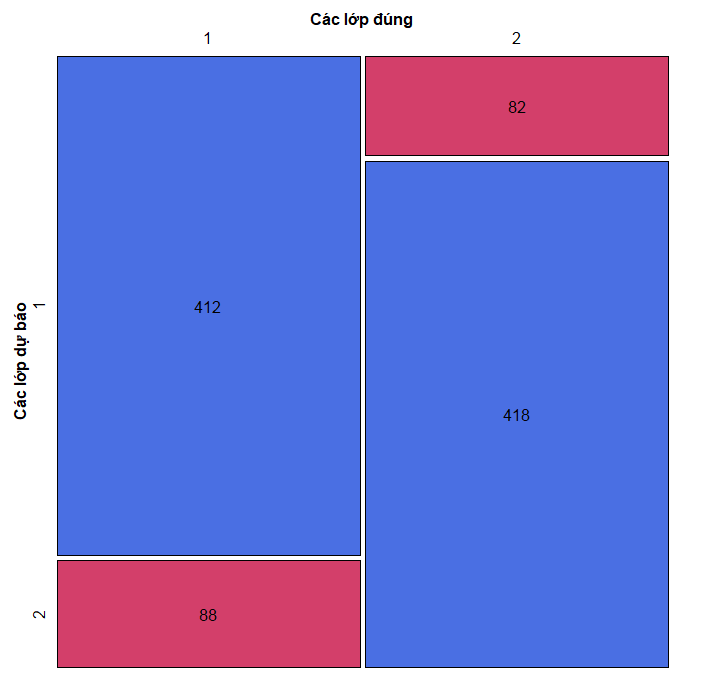
\includegraphics[width=0.6\textwidth]{image/confusion_matrix_test.png}
    \caption{Ma trận lỗi dùng để đánh giá kết quả phân loại của mô hình LDA.}
    \label{fig:confusion_matrix_lda}
\end{figure}

Từ ma trận lỗi hiển thị trên Hình \ref{fig:confusion_matrix_lda}, ta xác định được số lượng các mẫu phân loại đúng và phân loại sai tương ứng của hai lớp. Cụ thể, số mẫu thuộc lớp $C_1$ phân loại đúng là $n_{11} = 412$, số mẫu phân loại sai sang lớp $C_2$ là $n_{21} = 88$. Đối với lớp $C_2$, số mẫu phân loại đúng là $n_{22} = 418$ và số mẫu phân loại sai sang lớp $C_1$ là $n_{12} = 82$.

Tỷ lệ lỗi thực nghiệm (Tỷ lệ phân loại lỗi - $\widehat{\mathrm{TPM}}$) được tính toán cụ thể như sau
\[
\widehat{\mathrm{TPM}}
=
\frac{n_{12}+n_{21}}{n}
=
\frac{82 + 88}{1000}
=
\frac{170}{1000}
=
0{,}170 \quad (17{,}0\%).
\]
Độ chính xác tổng thể của sự phân lớp (the overall accuracy) của mô hình LDA đạt
\[
\text{Overall Accuracy}
=
1 - \widehat{\mathrm{TPM}}
=
1 - 0{,}170
=
0{,}830 \quad (83{,}0\%).
\]
Các chỉ số độ chính xác phân loại (Recall) và độ chính xác tiên đoán (Precision) cho từng lớp $C_j$ ($j = 1, 2$) được xác định theo các công thức
\begin{itemize}
	\item \textbf{Recall:} $P(\hat{C}_j\mid C_j) = \frac{n_{jj}}{n_{\bullet j}}$
	\item \textbf{Precision:} $P(C_j\mid \hat{C}_j) = \frac{n_{jj}}{n_{j\bullet}}$
\end{itemize}

Kết quả tính toán cụ thể được tóm tắt trong Bảng \ref{tab:metrics_summary}

\begin{table}[H]
	\centering
	\renewcommand{\arraystretch}{1.5}
	\begin{tabular}{|c|c|c|}
		\hline
		\textbf{Lớp} & \textbf{Recall} $P(\hat{C}_j \mid C_j)$ & \textbf{Precision} $P(C_j \mid \hat{C}_j)$ \\
		\hline
		\textbf{$C_1$} & $\frac{412}{500} = 82{,}4\%$ & $\frac{412}{494} \approx 83{,}40\%$ \\
		\hline
		\textbf{$C_2$} & $\frac{418}{500} = 83{,}6\%$ & $\frac{418}{506} \approx 82{,}61\%$ \\
		\hline
	\end{tabular}
	\caption{Các chỉ số Recall và Precision cho trường hợp hai lớp ít chồng lấp}
	\label{tab:metrics_summary}
\end{table}

Từ ma trận lỗi theo tần số, ta tính được các tỷ lệ tương ứng bằng công thức
\[
p_{ij}=\frac{n_{ij}}{n},\qquad i,j=1,2.
\]

Với $n=1000$, ta có
\[
p_{11}=\frac{412}{1000}=0{,}412,\qquad
p_{12}=\frac{82}{1000}=0{,}082,
\]
\[
p_{21}=\frac{88}{1000}=0{,}088,\qquad
p_{22}=\frac{418}{1000}=0{,}418.
\]

Ngoài ra,
\[
p_{1\bullet}=p_{11}+p_{12}=0{,}412+0{,}082=0{,}494,
\]
\[
p_{2\bullet}=p_{21}+p_{22}=0{,}088+0{,}418=0{,}506,
\]
và
\[
p_{\bullet 1}=p_{11}+p_{21}=0{,}412+0{,}088=0{,}500,
\]
\[
p_{\bullet 2}=p_{12}+p_{22}=0{,}082+0{,}418=0{,}500.
\]

Do đó, ma trận lỗi theo tỷ lệ được cho bởi bảng sau
\begin{table}[H]
	\centering
	\begin{tabular}{|c|cc|c|}
		\hline
		\multirow{2}{*}{Các lớp dự báo} 
		& \multicolumn{2}{c|}{Các lớp đúng} 
		& \multirow{2}{*}{Tổng cộng} \\ \cline{2-3}
		& $C_1$ & $C_2$ & \\ \hline
		$\hat{C}_1$ & $0{,}412$ & $0{,}082$ & $0{,}494$ \\
		$\hat{C}_2$ & $0{,}088$ & $0{,}418$ & $0{,}506$ \\ \hline
		Tổng cộng & $0{,}500$ & $0{,}500$  & $1{,}000$ \\ \hline
	\end{tabular}
	\caption{Ma trận lỗi theo tỷ lệ của mô hình LDA trong trường hợp hai lớp ít chồng lấp.}
	\label{tab:MaTranLoiTyLe_LDA_ItChongLap}
\end{table}

Trong phần trước, ta đã xét trường hợp hai lớp chuẩn hai chiều có vùng giao nhau nhất định. Để thấy rõ hơn hạn chế của bộ phân loại tuyến tính khi dữ liệu có mức độ chồng lấn cao, ta tiếp tục xét một mô phỏng khác, trong đó hai lớp có tâm rất gần nhau và có cùng ma trận hiệp phương sai.

\subsection{Mô phỏng trường hợp hai lớp chồng lấp nhiều}
Xét bài toán phân loại với dữ liệu hai chiều $(d=2)$. Dữ liệu được sinh ngẫu nhiên từ hai phân phối chuẩn hai chiều có cùng ma trận hiệp phương sai.

Thiết lập các tham số của dữ liệu mô phỏng như sau
\[
n_1=n_2=500.
\]
\[
\bm{\mu}_1=
\begin{pmatrix}
	3\\
	3
\end{pmatrix},
\qquad
\bm{\mu}_2=
\begin{pmatrix}
	3{,}2\\
	2{,}5
\end{pmatrix}.
\]
\[
\Sigma
=
\begin{pmatrix}
	2 & 1\\
	1 & 2
\end{pmatrix}.
\]
Từ các tham số đã thiết lập, ta đã tính được
\[
\bm{\beta}_{\text{opt}}
=
\Sigma^{-1}(\bm{\mu}_1-\bm{\mu}_2)
=
\begin{pmatrix}
	-0{,}3\\
	0{,}4
\end{pmatrix}.
\]

Do hai lớp có xác suất tiên nghiệm bằng nhau, biên LDA lý thuyết đi qua trung điểm của hai vectơ trung bình
\[
\frac{\bm{\mu}_1+\bm{\mu}_2}{2}
=
\begin{pmatrix}
	3{,}1\\
	2{,}75
\end{pmatrix}.
\]

Vì vậy, biên LDA lý thuyết được xác định bởi
\[
\bm{\beta}_{\text{opt}}^T
\left(
\bm{x}_{\text{bnd}}
-
\frac{\bm{\mu}_1+\bm{\mu}_2}{2}
\right)
=
0.
\]

Thay các giá trị đã tính vào, ta có
\[
\begin{pmatrix}
	-0{,}3 & 0{,}4
\end{pmatrix}
\left[
\begin{pmatrix}
	x_1\\
	x_2
\end{pmatrix}
-
\begin{pmatrix}
	3{,}1\\
	2{,}75
\end{pmatrix}
\right]
=
0.
\]

Suy ra phương trình biên LDA lý thuyết là
\[
-0{,}3x_1+0{,}4x_2-0{,}17=0.
\]

Tương đương,
\[
x_2=0{,}425+0{,}75x_1.
\]

Biên LDA lý thuyết này được dùng để so sánh với biên LDA thực nghiệm được ước lượng từ dữ liệu mô phỏng.

Từ các tham số mô phỏng trên, ta sinh ngẫu nhiên tập dữ liệu của hai lớp
\[
D_1=\{\bm{x}_{11},\bm{x}_{21},\ldots,\bm{x}_{n_1 1}\},
\qquad
D_2=\{\bm{x}_{12},\bm{x}_{22},\ldots,\bm{x}_{n_2 2}\}.
\]

Từ dữ liệu mô phỏng, ta tính trung bình mẫu \(\hat{\bm{\mu}}_1, \hat{\bm{\mu}}_2\) và ma trận hiệp phương sai mẫu của từng lớp. \[ \hat{\pi}_1=\hat{\pi}_2=0{,}5, \] \[ \hat{\bm{\mu}}_1 = \begin{pmatrix} 2{,}9716\\ 3{,}0225 \end{pmatrix}, \qquad \hat{\bm{\mu}}_2 = \begin{pmatrix} 3{,}2101\\ 2{,}5101 \end{pmatrix}, \] 
Ma trận hiệp phương sai mẫu của lớp 1 và lớp 2 lần lượt là \[ \hat{\Sigma}_1 = \begin{pmatrix} 2{,}1251 & 0{,}9023\\ 0{,}9023 & 1{,}9656 \end{pmatrix}, \qquad \hat{\Sigma}_2 = \begin{pmatrix} 1{,}7762 & 0{,}8397\\ 0{,}8397 & 1{,}9534 \end{pmatrix}. \] Từ đó, ma trận hiệp phương sai mẫu gộp được ước lượng bởi \[ \hat{\Sigma} = \begin{pmatrix} 1{,}9507 & 0{,}8710\\ 0{,}8710 & 1{,}9595 \end{pmatrix}. \]
Khi đó, phương chiếu Fisher thực nghiệm được xác định bởi \[ \bm{b}_{\text{opt}} = \hat{\Sigma}^{-1}(\hat{\bm{\mu}}_1-\hat{\bm{\mu}}_2) = \begin{pmatrix} -0{,}2982\\ 0{,}3940 \end{pmatrix}. \] Đường phân loại tuyến tính của LDA có dạng \[ \bm{b}_{\text{opt}}^T \left( \bm{x}_{\text{bnd}} - \frac{\hat{\bm{\mu}}_1 + \hat{\bm{\mu}}_2}{2} \right) = 0. \] Trung điểm của hai vectơ trung bình mẫu là \[ \frac{\hat{\bm{\mu}}_1+\hat{\bm{\mu}}_2}{2} = \begin{pmatrix} 3{,}0908\\ 2{,}7663 \end{pmatrix}. \] Thay số vào, ta được \[ \begin{pmatrix} -0{,}2982 & 0{,}3940 \end{pmatrix} \left[ \bm{x} - \begin{pmatrix} 3{,}0908\\ 2{,}7663 \end{pmatrix} \right] = 0. \] Tương đương, \[ -0{,}2982x_1+0{,}3940x_2-0{,}1684=0. \] Hay \[ x_2=0{,}4274+0{,}7567x_1. \]

\begin{figure}[H]
	\centering
	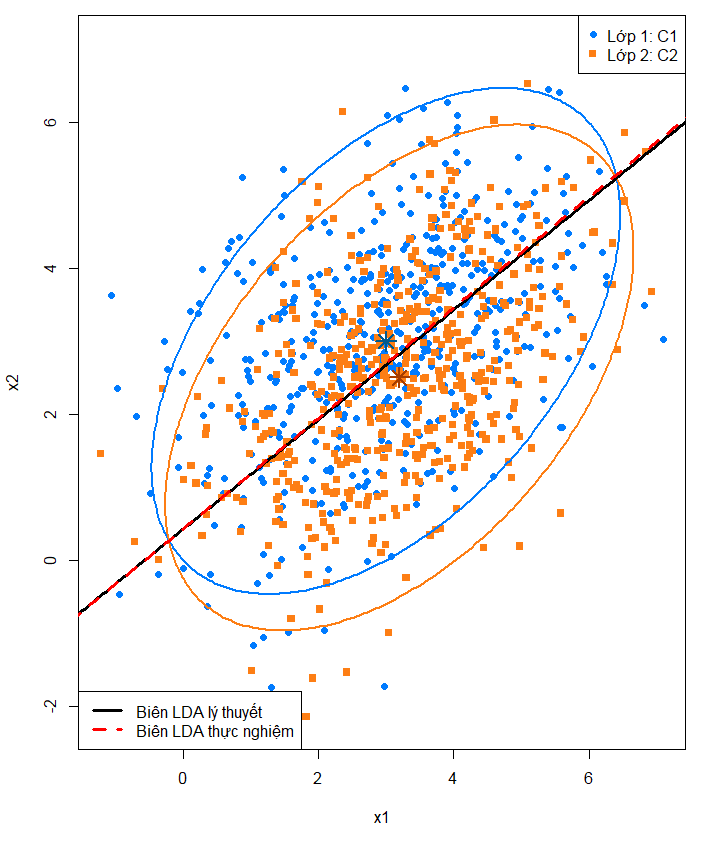
\includegraphics[width=0.8\textwidth]{image/normal_dis_2_classes_overlap_test.png}
	\caption{Phân bố mẫu của hai lớp chuẩn hai chiều có tương quan dương và mức độ chồng lấp lớn.}
	\label{fig:2d_normal_overlap}
\end{figure}

Từ Hình~\ref{fig:2d_normal_overlap}, có thể thấy hai lớp dữ liệu chồng lấn mạnh trong không gian hai chiều. Nguyên nhân chính là do khoảng cách giữa hai vectơ trung bình \[ \hat{\bm{\mu}}_1 = \begin{pmatrix} 2{,}9716\\ 3{,}0225 \end{pmatrix}, \qquad \hat{\bm{\mu}}_2 = \begin{pmatrix} 3{,}2101\\ 2{,}5101 \end{pmatrix} \] khá nhỏ so với độ phân tán của dữ liệu được xác định bởi ma trận hiệp phương sai mẫu gộp \[ \hat{\Sigma} = \begin{pmatrix} 1{,}9507 & 0{,}8710\\ 0{,}8710 & 1{,}9595 \end{pmatrix}. \] Khoảng cách Euclid giữa hai tâm chỉ là \[ \|\hat{\bm{\mu}}_1-\hat{\bm{\mu}}_2\| = \sqrt{(2{,}9716-3{,}2101)^2+(3{,}0225-2{,}5101)^2} \] \[ = \sqrt{(-0{,}2385)^2+(0{,}5124)^2} = \sqrt{0{,}0569+0{,}2626} = \sqrt{0{,}3195} \approx 0{,}5652. \] Trong khi đó, phương sai theo từng trục đều xấp xỉ \(2\), cho thấy độ phân tán của mỗi lớp tương đối lớn. Vì vậy, mặc dù hai lớp có hai tâm khác nhau, phần lớn các điểm dữ liệu vẫn nằm xen kẽ trong cùng một vùng không gian.

\hspace*{0.5cm}Đường LDA vẫn chia không gian thành hai miền quyết định tuyến tính. Tuy nhiên, do vùng giao nhau giữa hai phân phối quá lớn, nhiều điểm của lớp $C_1$ nằm về phía miền quyết định của lớp $C_2$ và ngược lại. Đây là nguyên nhân làm tăng tỷ lệ phân loại sai.

Để đánh giá kết quả phân loại, ta tiếp tục sử dụng ma trận lỗi.

\begin{figure}[H]
	\centering
	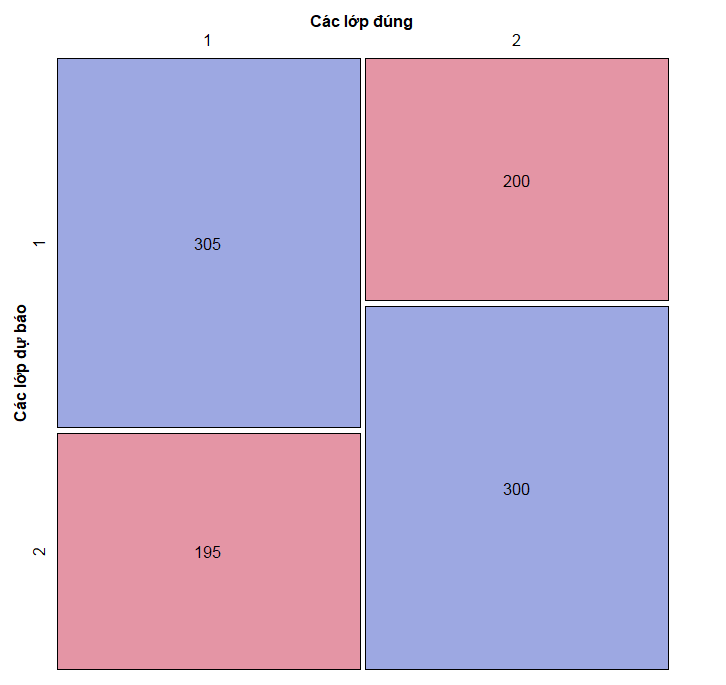
\includegraphics[width=0.6\textwidth]{image/confusion_matrix_overlap_test.png}
	\caption{Ma trận lỗi của mô hình LDA trong trường hợp hai lớp chồng lấp nhiều.}
	\label{fig:confusion_matrix_overlap}
\end{figure}

Từ ma trận lỗi hiển thị trên Hình~\ref{fig:confusion_matrix_overlap}, ta xác định được số lượng các mẫu phân loại đúng và phân loại sai tương ứng của hai lớp. Cụ thể, số mẫu thuộc lớp $C_1$ phân loại đúng là $n_{11}=305$, số mẫu phân loại sai sang lớp $C_2$ là $n_{21}=195$. Đối với lớp $C_2$, số mẫu phân loại đúng là $n_{22}=300$ và số mẫu phân loại sai sang lớp $C_1$ là $n_{12}=200$.

Tỷ lệ lỗi thực nghiệm được tính bởi
\[
\widehat{\mathrm{TPM}}
=
\frac{n_{12}+n_{21}}{n}
=
\frac{200+195}{1000}
=
\frac{395}{1000}
=
0{,}395.
\]

Hay tương đương,
\[
\widehat{\mathrm{TPM}}=39{,}5\%.
\]

Độ chính xác phân loại toàn cục của mô hình LDA là
\[
\text{Overall Accuracy}
=
1-\widehat{\mathrm{TPM}}
=
1-0{,}395
=
0{,}605.
\]

Hay,
\[
\text{Overall Accuracy}=60{,}5\%.
\]
Các chỉ số độ chính xác phân loại (Recall) và độ chính xác tiên đoán (Precision) cho từng lớp $C_j$ ($j = 1, 2$) được xác định theo các công thức:
\begin{itemize}
	\item \textbf{Recall:} $P(\hat{C}_j\mid C_j) = \frac{n_{jj}}{n_{\bullet j}}$
	\item \textbf{Precision:} $P(C_j\mid \hat{C}_j) = \frac{n_{jj}}{n_{j\bullet}}$
\end{itemize}

Kết quả tính toán cụ thể được tóm tắt trong Bảng \ref{tab:metrics_summary}

\begin{table}[htpb]
	\centering
	\renewcommand{\arraystretch}{1.5}
	\begin{tabular}{|c|c|c|}
		\hline
		\textbf{Lớp} & \textbf{Recall} $P(\hat{C}_j \mid C_j)$ & \textbf{Precision} $P(C_j \mid \hat{C}_j)$ \\
		\hline
		\textbf{$C_1$} & $\frac{305}{500} = 61{,}0\%$ & $\frac{305}{505} \approx 60{,}40\%$ \\
		\hline
		\textbf{$C_2$} & $\frac{300}{500} = 60{,}0\%$ & $\frac{300}{495} \approx 60{,}61\%$ \\
		\hline
	\end{tabular}
	\caption{Các chỉ số Recall và Precision cho trường hợp hai lớp chồng lấp nhiều}
	\label{tab:metrics_summary}
\end{table}

Từ ma trận lỗi theo tần số, ta tính được các tỷ lệ tương ứng bằng công thức $p_{ij} = \frac{n_{ij}}{n}$ ($i,j=1,2$). Với $n=1000$, ta có các tỷ lệ thành phần và các tổng lề như sau
\begin{align*}
	p_{11} &= \frac{305}{1000} = 0{,}305, & p_{12} &= \frac{200}{1000} = 0{,}200, & p_{1\bullet} &= 0{,}305 + 0{,}200 = 0{,}505 \\
	p_{21} &= \frac{195}{1000} = 0{,}195, & p_{22} &= \frac{300}{1000} = 0{,}300, & p_{2\bullet} &= 0{,}195 + 0{,}300 = 0{,}495 \\
	p_{\bullet 1} &= 0{,}305 + 0{,}195 = 0{,}500, & p_{\bullet 2} &= 0{,}200 + 0{,}300 = 0{,}500
\end{align*}

Do đó, ma trận lỗi theo tỷ lệ được cho bởi bảng sau
\begin{table}[H]
	\centering
	\begin{tabular}{|c|cc|c|}
		\hline
		\multirow{2}{*}{Các lớp dự báo} 
		& \multicolumn{2}{c|}{Các lớp đúng} 
		& \multirow{2}{*}{Tổng cộng} \\ \cline{2-3}
		& $C_1$ & $C_2$ & \\ \hline
		$\hat{C}_1$ & $0{,}305$ & $0{,}200$ & $0{,}505$ \\
		$\hat{C}_2$ & $0{,}195$ & $0{,}300$ & $0{,}495$ \\ \hline
		Tổng cộng & $0{,}500$ & $0{,}500$  & $1{,}000$ \\ \hline
	\end{tabular}
	\caption{Ma trận lỗi theo tỷ lệ của mô hình LDA trong trường hợp hai lớp chồng lấp nhiều.}
	\label{tab:MaTranLoiTyLe_LDA_ChongLanNhieu}
\end{table}

Kết quả này cho thấy khi hai lớp có mức độ chồng lấn lớn, hiệu quả phân loại của LDA giảm đáng kể. Mặc dù LDA vẫn xác định được một đường phân loại tuyến tính, đường này không thể tách hoàn toàn hai lớp do phần lớn các quan sát của hai lớp nằm xen kẽ trong cùng một vùng không gian. Sai số phân loại $39{,}5\%$ phản ánh mức độ khó của bài toán, xuất phát từ việc hai phân phối có tâm rất gần nhau so với độ phân tán của dữ liệu. Trong trường hợp này, sai số không chủ yếu đến từ việc lựa chọn sai dạng mô hình, vì hai lớp vẫn được sinh từ các phân phối chuẩn có cùng ma trận hiệp phương sai. Nguyên nhân chính là vùng chồng lấn giữa hai phân phối quá lớn, làm cho nhiều điểm thuộc lớp $C_1$ có đặc trưng gần giống với lớp $C_2$ và ngược lại. Do đó, ngay cả biên quyết định tuyến tính tối ưu theo LDA cũng không thể đạt độ chính xác cao.

\hspace*{0.5cm}Trường hợp mô phỏng này cho thấy khi hai phân phối chuẩn có tâm quá gần nhau so với độ phân tán nội tại, vùng chồng lấn giữa hai lớp trở nên rất lớn. Khi đó, ngay cả khi giả thiết của LDA được thỏa mãn, tức là hai lớp có cùng ma trận hiệp phương sai và biên Bayes là tuyến tính, mô hình vẫn không thể phân loại tốt.

Qua các mô phỏng trên, có thể thấy hiệu quả của phương pháp Fisher LDA phụ thuộc mạnh vào cấu trúc phân bố của dữ liệu. Khi hai lớp có tâm cách xa nhau và mức độ chồng lấn nhỏ, LDA xác định được một biên phân loại tuyến tính tương đối tốt, cho tỷ lệ phân loại sai thấp. Ngược lại, khi hai lớp có tâm gần nhau, phương sai lớn hoặc vùng chồng lấn giữa hai phân phối trở nên đáng kể, tỷ lệ lỗi phân loại tăng lên rõ rệt.

\hspace*{0.5cm}Trường hợp hai lớp chồng lấn ít trong ví dụ đầu cho thấy LDA có thể đạt độ chính xác khá cao, chẳng hạn tỷ lệ lỗi thực nghiệm khoảng $17{,}0\%$. Trong khi đó, ở trường hợp hai lớp chồng lấn mạnh, tỷ lệ lỗi tăng lên đến $39{,}5\%$, tương ứng độ chính xác chỉ còn $60{,}5\%$. Sự khác biệt này minh họa rõ rằng khả năng phân tách của LDA không chỉ phụ thuộc vào việc có tồn tại biên tuyến tính hay không, mà còn phụ thuộc vào mức độ tách biệt thực sự giữa các phân phối lớp.

\hspace*{0.5cm}Như vậy, Fisher LDA là một phương pháp hiệu quả khi dữ liệu có cấu trúc lớp tương đối rõ ràng và thỏa mãn các giả thiết của mô hình. Tuy nhiên, trong các bài toán mà các lớp chồng lấn mạnh, ngay cả biên tuyến tính tối ưu cũng khó đạt hiệu quả phân loại cao. Điều này cho thấy khi áp dụng LDA trong thực hành, cần xem xét đồng thời các yếu tố như khoảng cách giữa các tâm lớp, độ phân tán của dữ liệu các nhóm.


\subsection{Mô phỏng trường hợp hai lớp tách biệt hoàn toàn}

Xét bài toán phân loại với dữ liệu hai chiều $(d=2)$ tương tự nhưng trong điều kiện hai phân phối có khoảng cách tâm (trung bình) đủ lớn.

Thiết lập các tham số của dữ liệu mô phỏng như sau
\[
n_1=n_2=500.
\]
\[
\bm{\mu}_1=
\begin{pmatrix}
	3\\
	3
\end{pmatrix},
\qquad
\bm{\mu}_2=
\begin{pmatrix}
	13\\
	3
\end{pmatrix}.
\]
\[
\Sigma
=
\begin{pmatrix}
	2 & 0\\
	0 & 2
\end{pmatrix}.
\]

Do các phần tử ngoài đường chéo của ma trận hiệp phương sai bằng $0$, ta có
\[
\sigma_{12}=\sigma_{21}=0.
\]
Điều này cho thấy hai biến đặc trưng $x_1$ và $x_2$ không có tương quan tuyến tính. Đồng thời, do hai phần tử trên đường chéo chính bằng nhau, tức là
\[
\sigma_1^2=\sigma_2^2=2,
\]
nên mức độ phân tán theo hai hướng $x_1$ và $x_2$ là như nhau. Vì vậy, các đám mây điểm của hai lớp có dạng gần tròn.

Trong trường hợp này, do hai lớp có cùng ma trận hiệp phương sai và cùng xác suất tiên nghiệm, biên quyết định LDA tương ứng với tập hợp các điểm có khoảng cách Mahalanobis đến hai tâm bằng nhau. Tuy nhiên, vì
\[
\Sigma=2\mathbb{I},
\]
khoảng cách Mahalanobis chỉ khác khoảng cách Euclid một hệ số tỷ lệ. Do đó, biên quyết định LDA chính là đường trung trực của đoạn nối hai tâm $\bm{\mu}_1$ và $\bm{\mu}_2$.


Trung điểm của hai vectơ trung bình là
\[
\bm{M}
=
\frac{\bm{\mu}_1+\bm{\mu}_2}{2}
=
\begin{pmatrix}
	\frac{3+13}{2}\\
	\frac{3+3}{2}
\end{pmatrix}
=
\begin{pmatrix}
	8\\
	3
\end{pmatrix}.
\]

Vì hai tâm có cùng tung độ và chỉ khác nhau theo phương $x_1$, đoạn nối hai tâm là một đoạn thẳng nằm ngang. Do đó, đường trung trực của đoạn nối hai tâm là đường thẳng đứng đi qua hoành độ của trung điểm:
\[
x_1=8.
\]

Mặt khác, từ dữ liệu mô phỏng, ta tính trung bình mẫu \(\hat{\bm{\mu}}_1, \hat{\bm{\mu}}_2\). 
\[
\hat{\pi}_1=\hat{\pi}_2=0{,}5.
\]
\[
\hat{\bm{\mu}}_1
=
\begin{pmatrix}
	2{,}9491\\
	2{,}9966
\end{pmatrix},
\qquad
\hat{\bm{\mu}}_2
=
\begin{pmatrix}
	12{,}9999\\
	3{,}0117
\end{pmatrix}.
\]
Ma trận hiệp phương sai mẫu ước lượng của lớp $1$ và lớp $2$ lần lượt là \[ \hat{\Sigma}_1 = \begin{pmatrix} 2{,}2861 & 0{,}0921\\ 0{,}0921 & 1{,}9651 \end{pmatrix}, \qquad \hat{\Sigma}_2 = \begin{pmatrix} 2{,}0503 & -0{,}1023\\ -0{,}1023 & 1{,}8030 \end{pmatrix}. \] Từ hai ma trận hiệp phương sai mẫu trên, ta thu được ma trận hiệp phương sai mẫu gộp \[ \hat{\Sigma} = \begin{pmatrix} 2{,}1682 & -0{,}0051\\ -0{,}0051 & 1{,}8841 \end{pmatrix}. \]

Khi đó, phương chiếu Fisher thực nghiệm được xác định bởi
\[
\bm{b}_{\text{opt}}
=
\hat{\Sigma}^{-1}
(\hat{\bm{\mu}}_1-\hat{\bm{\mu}}_2)
=
\begin{pmatrix}
	-4{,}6356\\
	-0{,}0205
\end{pmatrix}.
\]

Đường phân loại tuyến tính của LDA có dạng
\[
\bm{b}_{\text{opt}}^T
\left(
\bm{x}_{\text{bnd}}
-
\frac{\hat{\bm{\mu}}_1+\hat{\bm{\mu}}_2}{2}
\right)
=0.
\]

Trung điểm của hai vectơ trung bình mẫu là
\[
\frac{\hat{\bm{\mu}}_1+\hat{\bm{\mu}}_2}{2}
=
\begin{pmatrix}
	7{,}9745\\
	3{,}0041
\end{pmatrix}.
\]

Thay số vào, ta được
\[
\begin{pmatrix}
	-4{,}6356 & -0{,}0205
\end{pmatrix}
\left[
\bm{x}
-
\begin{pmatrix}
	7{,}9745\\
	3{,}0041
\end{pmatrix}
\right]
=0.
\]

Tương đương, phương trình biên LDA thực nghiệm là \[ -4{,}6356x_1 - 0{,}0205x_2 + 37{,}0283 = 0. \] Nếu viết dưới dạng \(x_2=a+bx_1\), ta thu được \[ x_2 \approx 1802{,}3010 - 225{,}6309x_1. \] Tuy nhiên, dạng biểu diễn này không thật sự thuận tiện để diễn giải vì hệ số của \(x_2\) trong phương trình tổng quát rất nhỏ so với hệ số của \(x_1\), cụ thể \[ |-0{,}0205| \ll |-4{,}6356|. \] Điều này cho thấy đường biên phân loại gần như là một đường thẳng đứng. Do đó, để thấy rõ vị trí của biên quyết định, ta có thể xấp xỉ bằng cách bỏ qua hạng tử chứa \(x_2\). Khi đó, \[ -4{,}6356x_1+37{,}0283 \approx 0, \] suy ra \[ x_1 \approx \frac{37{,}0283}{4{,}6356} \approx 7{,}9878. \] Như vậy, biên LDA thực nghiệm gần như là đường thẳng đứng đi qua \(x_1 \approx 7{,}9878\), phù hợp với việc hai lớp chủ yếu tách biệt theo trục \(x_1\).

Mặt khác, do ma trận hiệp phương sai mẫu gộp
\[
\hat{\Sigma}
=
\begin{pmatrix}
	2{,}1682 & -0{,}0051\\
	-0{,}0051 & 1{,}8841
\end{pmatrix}
\]
xấp xỉ ma trận $2\mathbb{I}$, nên
\[
\hat{\Sigma}^{-1}
\approx
\frac{1}{2}\mathbb{I}.
\]

Vì vậy,
\[
\bm{b}_{\text{opt}}
=
\hat{\Sigma}^{-1}
(\hat{\bm{\mu}}_1-\hat{\bm{\mu}}_2)
\approx
\frac{1}{2}
(\hat{\bm{\mu}}_1-\hat{\bm{\mu}}_2).
\]
Có
\[
\hat{\bm{\mu}}_1-\hat{\bm{\mu}}_2
=
\begin{pmatrix}
	2{,}9491\\
	2{,}9966
\end{pmatrix}
-
\begin{pmatrix}
	12{,}9999\\
	3{,}0117
\end{pmatrix}
=
\begin{pmatrix}
	-10{,}0508\\
	-0{,}0150
\end{pmatrix},
\]
nên
\[
\bm{b}_{\text{opt}}
\approx
\frac{1}{2}
\begin{pmatrix}
	-10{,}0508\\
	-0{,}0150
\end{pmatrix}
=
\begin{pmatrix}
	-5{,}0254\\
	-0{,}0075
\end{pmatrix}.
\]

Do đó, phương pháp tuyến của biên phân loại cùng phương với đoạn nối hai tâm. Vì đoạn nối hai tâm song song với trục $x_1$, nên biên phân loại vuông góc với trục này và có dạng một đường thẳng đứng.

\begin{figure}[H]
	\centering
	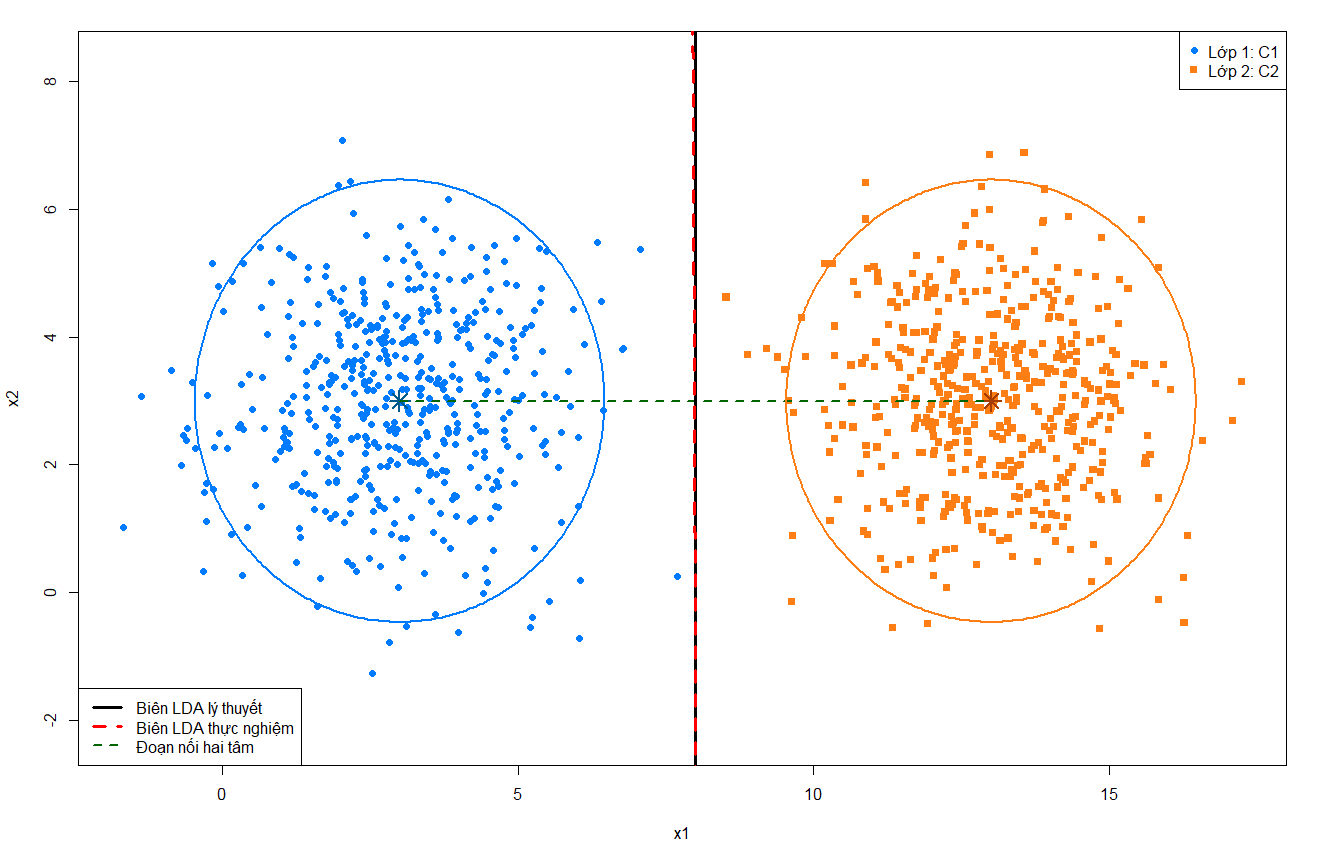
\includegraphics[width=0.75\textwidth]{image/circular_separable_2_classes.png}
	\caption{Hai đám mây chuẩn hai chiều không tương quan, có dạng tròn và được phân tách bởi biên LDA gần với đường trung trực của hai tâm.}
	\label{fig:circular_separable_class}
\end{figure}

Từ Hình~\ref{fig:circular_separable_class}, có thể thấy hai lớp tạo thành hai cụm dữ liệu gần tròn, tách biệt rõ ràng trong không gian hai chiều. Đường phân loại LDA gần như là một đường thẳng đứng nằm giữa hai cụm dữ liệu và gần với đường trung trực của đoạn nối hai tâm. Trong trường hợp này, biên phân loại không chỉ là một đường thẳng tối ưu theo LDA mà còn có ý nghĩa hình học rất trực quan: mỗi điểm dữ liệu được gán vào lớp có tâm gần nó hơn.

Kết quả phân loại cho thấy không có điểm dữ liệu nào bị phân loại sai. Ma trận lỗi thực nghiệm có dạng
\[
\begin{array}{c|cc}
	& \text{Dự đoán } C_1 & \text{Dự đoán } C_2\\
	\hline
	\text{Thực tế } C_1 & 500 & 0\\
	\text{Thực tế } C_2 & 0 & 500
\end{array}
\]
\begin{figure}[H]
	\centering
	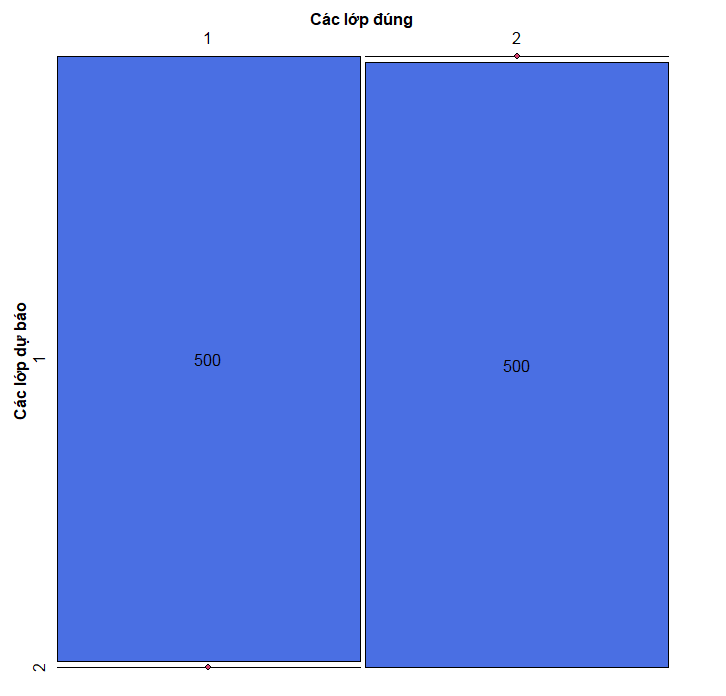
\includegraphics[width=0.75\textwidth]{image/confusion_matrix_separable_test.png}
	\caption{Ma trận lỗi của mô hình LDA trong trường hợp hai lớp tách biệt hoàn toàn.}
	\label{fig:confusion_matrix_separable_test}
\end{figure}
Từ ma trận trên, các phần tử ngoài đường chéo chính đều bằng $0$, tức là
\[
n_{12}=0,\qquad n_{21}=0.
\]

Do đó, tỷ lệ lỗi thực nghiệm là
\[
\widehat{\mathrm{TPM}}
=
\frac{n_{12}+n_{21}}{n}
=
\frac{0+0}{1000}
=
0.
\]

Độ chính xác phân loại đạt
\[
\text{Overall Accuracy}
=
1-\widehat{\mathrm{TPM}}
=
1-0
=
1.
\]

Hay tương đương
\[
\text{Overall Accuracy}=100\%.
\]
Do $n_{12}=n_{21}=0$, không có quan sát nào bị phân loại sai. Vì vậy, đối với cả hai lớp, các chỉ số Recall và Precision đều đạt $100\%$
\[
\text{Recall}_{C_1}
=
\text{Recall}_{C_2}
=
\text{Precision}_{C_1}
=
\text{Precision}_{C_2}
=
100\%.
\]
Kết quả phân loại hoàn hảo này được thể hiện rất rõ qua ma trận lỗi theo tỷ lệ dưới đây
\begin{table}[H]
	\centering
	\begin{tabular}{|c|cc|c|}
		\hline
		\multirow{2}{*}{Các lớp dự báo} 
		& \multicolumn{2}{c|}{Các lớp đúng} 
		& \multirow{2}{*}{Tổng cộng} \\ \cline{2-3}
		& $C_1$ & $C_2$ & \\ \hline
		$\hat{C}_1$ & $0{,}500$ & $0$ & $0{,}500$ \\
		$\hat{C}_2$ & $0$ & $0{,}500$ & $0{,}500$ \\ \hline
		Tổng cộng & $0{,}500$ & $0{,}500$  & $1{,}000$ \\ \hline
	\end{tabular}
	\caption{Ma trận lỗi theo tỷ lệ của mô hình LDA trong trường hợp hai lớp tách biệt hoàn toàn.}
	\label{tab:MaTranLoiTyLe_LDA_TachBietHoanToan}
\end{table}
Trường hợp này cho thấy khi hai lớp có cùng ma trận hiệp phương sai dạng $\sigma^2 \mathbb{I}$, không có tương quan giữa các biến đặc trưng và hai tâm cách xa nhau, LDA đưa ra một biên phân loại rất trực quan: đường trung trực của đoạn nối hai tâm. Đây là một trường hợp đặc biệt trong đó quy tắc phân loại LDA tương đương với quy tắc gán điểm vào lớp có tâm gần nhất theo khoảng cách Euclid. Khi khoảng cách giữa hai tâm đủ lớn so với độ phân tán trong từng lớp, hai đám mây dữ liệu được phân tách hoàn toàn và tỷ lệ lỗi thực nghiệm bằng $0$.

%================3
\chapter*{Kết luận}
\addcontentsline{toc}{chapter}{Kết luận}
\markboth{Kết luận}{Kết luận}

\section*{1. Kết quả đạt được}

Đồ án đã trình bày cơ sở lý thuyết của phương pháp phân tích tách biệt tuyến tính Fisher trong bài toán phân loại mẫu thống kê. Trọng tâm của phương pháp là tìm một hướng chiếu tuyến tính sao cho khoảng cách giữa các lớp sau khi chiếu được làm lớn, đồng thời độ phân tán trong từng lớp được làm nhỏ. Từ đó, tiêu chuẩn Fisher được xây dựng dựa trên tỷ số giữa độ phân tán giữa lớp và độ phân tán trong lớp. Đối với trường hợp hai lớp, đồ án đã thiết lập các ma trận tán xạ trong lớp, tán xạ giữa lớp và đưa bài toán tối ưu Fisher về dạng thương Rayleigh. Qua đó, hướng chiếu tối ưu được xác định bởi \[ \bm{\beta}_{\text{opt}} \propto \Sigma_W^{-1}(\bm{\mu}_1-\bm{\mu}_2). \] Đây là kết quả cơ bản của Fisher LDA trong trường hợp hai lớp. Bên cạnh cách tiếp cận hình học, đồ án cũng đã trình bày cách tiếp cận theo lý thuyết quyết định Bayes. Trong trường hợp các lớp có phân phối chuẩn nhiều chiều và cùng ma trận hiệp phương sai, quy tắc Bayes dẫn đến hàm phân biệt tuyến tính. Do đó, biên quyết định giữa hai lớp là một siêu phẳng tuyến tính. Đồ án cũng chỉ ra rằng phương chiếu tối ưu của Fisher và phương pháp tuyến của biên quyết định Bayes đều cùng phương với \[ \Sigma^{-1}(\bm{\mu}_1-\bm{\mu}_2). \] Điều này cho thấy LDA vừa có ý nghĩa hình học, vừa có cơ sở xác suất từ lý thuyết Bayes. Ngoài phần lý thuyết, đồ án đã minh họa phương pháp LDA trên bộ dữ liệu Iris và dữ liệu mô phỏng hai chiều. Với dữ liệu Iris, kết quả cho thấy khi hai lớp có vùng chồng lấn thì vẫn xuất hiện sai số phân loại; ngược lại, khi hai lớp tách biệt rõ ràng thì LDA có thể phân loại chính xác hoàn toàn. Với dữ liệu mô phỏng, đồ án đã xét nhiều tình huống khác nhau: hai lớp chồng lấn vừa phải, hai lớp chồng lấn mạnh và hai lớp tách biệt hoàn toàn. Kết quả thực nghiệm cho thấy tỷ lệ lỗi phụ thuộc rõ rệt vào mức độ chồng lấn giữa các lớp. 

Như vậy, đồ án đã làm rõ được cơ sở toán học của Fisher LDA, chứng minh nghiệm tối ưu trong trường hợp hai lớp, trình bày sự tương đồng giữa Fisher LDA và quy tắc Bayes, đồng thời kiểm chứng bằng các ví dụ thực nghiệm. Các kết quả thu được cho thấy LDA là một phương pháp phân loại tuyến tính có nền tảng lý thuyết rõ ràng, đặc biệt hiệu quả khi dữ liệu có cấu trúc lớp tương đối tách biệt và giả thiết có cùng hiệp phương sai là phù hợp.

\section*{2. Một số vấn đề cần tiếp tục nghiên cứu}

Trong phạm vi đồ án, phương pháp LDA mới được khảo sát chủ yếu trong trường hợp hai lớp. Vì vậy, một hướng nghiên cứu tiếp theo là mở rộng LDA cho bài toán nhiều lớp, tức trường hợp \(K>2\). Khi đó, không gian chiếu tối ưu có số chiều tối đa là \(K-1\), giúp phân tách đồng thời nhiều lớp trong cùng một mô hình. Việc nghiên cứu LDA nhiều lớp sẽ làm rõ hơn khả năng mở rộng của phương pháp trong các bài toán phân loại thực tế có nhiều nhóm đối tượng.

Bên cạnh đó, có thể tiếp tục so sánh LDA với các phương pháp phân loại mẫu khác như hồi quy logistic, KNN, cây quyết định, SVM hoặc các mô hình học máy hiện đại. Qua đó, có thể xác định rõ hơn ưu điểm, hạn chế và điều kiện áp dụng phù hợp của LDA so với các phương pháp phân loại khác.

Đây là những hướng giúp hoàn thiện hơn việc nghiên cứu và đánh giá khả năng ứng dụng của LDA trong phân loại mẫu thống kê.


%Trong phạm vi đồ án, phương pháp LDA chủ yếu được khảo sát trong trường hợp hai lớp, dữ liệu có phân phối chuẩn nhiều chiều và các lớp có cùng ma trận hiệp phương sai. Đây là giả thiết thuận lợi giúp biên quyết định thu được có dạng tuyến tính. Tuy nhiên, trong các bài toán thực tế, dữ liệu thường có cấu trúc phức tạp hơn. Do đó, một hướng nghiên cứu tiếp theo là mở rộng việc khảo sát LDA trong các trường hợp dữ liệu không hoàn toàn thỏa mãn giả thiết Gaussian hoặc các lớp có ma trận hiệp phương sai khác nhau.
%
%Một hướng mở rộng tự nhiên là nghiên cứu phương pháp phân tích biệt thức bậc hai, tức Quadratic Discriminant Analysis (QDA). Khác với LDA, QDA cho phép mỗi lớp có một ma trận hiệp phương sai riêng. Khi đó, biên quyết định giữa các lớp nói chung không còn là siêu phẳng tuyến tính mà có dạng bậc hai. Việc so sánh LDA và QDA trên các bộ dữ liệu có mức độ chồng lấn khác nhau sẽ giúp đánh giá rõ hơn khi nào giả thiết cùng hiệp phương sai của LDA là phù hợp và khi nào cần dùng mô hình linh hoạt hơn.
%
%Ngoài ra, đồ án mới chỉ xét chủ yếu bài toán phân loại hai lớp. Trong các ứng dụng thực tế, số lớp thường lớn hơn hai. Vì vậy, có thể tiếp tục nghiên cứu LDA trong trường hợp nhiều lớp, tức là với $K>2$. Khi đó, không gian chiếu tối ưu của Fisher có số chiều tối đa là $K-1$, và bài toán không chỉ là tìm một hướng chiếu duy nhất mà là tìm một không gian con giúp phân tách đồng thời nhiều lớp. Đây là hướng mở rộng quan trọng để áp dụng LDA cho các bài toán phân loại đa lớp.
%
%Một vấn đề khác cần tiếp tục nghiên cứu là ảnh hưởng của số chiều dữ liệu đến hiệu quả của LDA. Khi số chiều đặc trưng lớn so với cỡ mẫu, ma trận phân tán trong lớp hoặc ma trận hiệp phương sai mẫu gộp có thể suy biến hoặc khó khả nghịch. Trong trường hợp này, công thức
%\[
%\beta_{\text{opt}}=\Sigma_W^{-1}(\mu_1-\mu_2)
%\]
%không còn áp dụng trực tiếp theo cách thông thường. Do đó, có thể nghiên cứu thêm các biến thể của LDA như regularized LDA, shrinkage LDA hoặc sử dụng giả nghịch đảo Moore--Penrose để xử lý trường hợp ma trận suy biến.
%
%Bên cạnh các mô phỏng đơn giản, một hướng phát triển tiếp theo là áp dụng LDA trên các bộ dữ liệu thực tế có quy mô lớn hơn. Trong đồ án, bộ dữ liệu Iris và dữ liệu mô phỏng đã giúp minh họa rõ ý nghĩa hình học và khả năng phân loại của LDA. Tuy nhiên, để đánh giá tính ứng dụng thực tế, cần thử nghiệm thêm trên các bộ dữ liệu thuộc nhiều lĩnh vực khác nhau như nhận dạng chữ viết tay, phân loại y sinh, tài chính, dữ liệu khách hàng hoặc các bài toán phân loại ảnh sau khi trích xuất đặc trưng.
%
%Ngoài việc đánh giá bằng ma trận lỗi và độ chính xác tổng thể, có thể mở rộng hệ thống đánh giá mô hình bằng nhiều chỉ số khác như precision, recall, F1-score, sensitivity, specificity và đường cong ROC. Đặc biệt, trong các bài toán dữ liệu mất cân bằng, độ chính xác tổng thể có thể không phản ánh đầy đủ chất lượng phân loại. Vì vậy, việc nghiên cứu các chỉ số đánh giá phù hợp hơn là cần thiết khi áp dụng LDA trong các bài toán thực tiễn.
%
%Một hướng nghiên cứu khác là so sánh LDA với các phương pháp phân loại tuyến tính và phi tuyến khác, chẳng hạn như hồi quy logistic, K lân cận gần nhất, cây quyết định, máy vector hỗ trợ và các phương pháp học máy hiện đại. Việc so sánh này có thể được thực hiện dựa trên cùng một bộ dữ liệu, cùng một quy trình chia tập huấn luyện và tập kiểm tra, từ đó đánh giá ưu điểm và hạn chế của LDA so với các phương pháp khác.
%
%Cuối cùng, có thể tiếp tục nghiên cứu vai trò của LDA như một phương pháp giảm chiều có giám sát. Trong hướng này, LDA không chỉ được dùng như một bộ phân loại mà còn được dùng để biến đổi dữ liệu sang một không gian mới có khả năng phân tách lớp tốt hơn. Việc kết hợp LDA với các phương pháp khác, chẳng hạn dùng LDA để giảm chiều trước khi áp dụng một bộ phân loại khác, cũng là một hướng nghiên cứu có ý nghĩa thực tiễn.
%
%Tóm lại, các hướng nghiên cứu tiếp theo có thể tập trung vào việc mở rộng LDA cho bài toán nhiều lớp, khảo sát các biến thể của LDA trong trường hợp ma trận hiệp phương sai không thuận lợi, so sánh LDA với các phương pháp phân loại khác, và áp dụng phương pháp này trên các bộ dữ liệu thực tế. Những hướng phát triển này sẽ giúp đánh giá đầy đủ hơn khả năng ứng dụng của LDA trong phân tích dữ liệu và học máy.

%====================================================
%               TÀI LIỆU THAM KHẢO
%====================================================
\clearpage
\addcontentsline{toc}{chapter}{Tài liệu tham khảo}
\begin{thebibliography}{99}

\bibitem{dangphuochuy2010}
Đặng Phước Huy,
\textit{Bài giảng tóm tắt -- Thống kê toán học},
Trường Đại học Đà Lạt, 2010.

\bibitem{dangphuochuy2023}
Đặng Phước Huy,
\textit{Bài giảng tóm tắt -- Phân tích thống kê nhiều chiều},
Trường Đại học Đà Lạt, 2023.

\bibitem{dangphuochuy2025}
Đặng Phước Huy,
\textit{Bài giảng tóm tắt -- Lý thuyết học thống kê},
Trường Đại học Đà Lạt, 2025.

\bibitem{ledinhphu2022}
Lê Đình Phú,
\textit{Suy diễn thống kê với phương pháp mẫu nhỏ (Khóa luận tốt nghiệp cử nhân toán học)},
Khoa Toán -- Tin học, Trường Đại học Đà Lạt, 2022.

\bibitem{fisher1936}
R. A. Fisher,
\textit{The Use of Multiple Measurements in Taxonomic Problems},
Annals of Eugenics, Vol. 7, No. 2, pp. 179--188, 1936.

\bibitem{bishop2006}
Christopher M. Bishop,
\textit{Pattern Recognition and Machine Learning},
Springer, 2006.

\bibitem{hastie2009}
Trevor Hastie, Robert Tibshirani, Jerome Friedman,
\textit{The Elements of Statistical Learning: Data Mining, Inference, and Prediction},
2nd ed., Springer, 2009.

\bibitem{johnson2007}
Johnson R. A., Wichern D. W.,
\textit{Applied Multivariate Statistical Analysis},
Pearson Prentice Hall, Pearson Education, Inc, 2007.

\bibitem{irisUCI}
R. A. Fisher,
\textit{Iris},
UCI Machine Learning Repository, 1936.
DOI: \url{https://doi.org/10.24432/C56C76}.

\end{thebibliography}

\end{document}